\documentclass[a4,12pt,english,twoside]{report}

% Define margins of document
\sloppy
\usepackage{geometry}
\geometry{verbose,a4paper,tmargin=30mm,bmargin=30mm,lmargin=30mm,rmargin=20mm}
%\geometry{verbose,a4paper,tmargin=30mm,bmargin=30mm,lmargin=30mm,rmargin=20mm}


% Set overall spacing
\usepackage{setspace}
\onehalfspacing

%\usepackage{mathrsfs}
\usepackage{graphicx}
\usepackage[centertags]{amsmath}
\usepackage{amsfonts,MnSymbol}
%\usepackage{amssymb}
\usepackage{amsthm}
\usepackage{cite}
%\usepackage{citesort}
%\usepackage{makeidx}
\usepackage{subfig}
\usepackage{float}
%\usepackage{subfloat}
\usepackage{rotating}
\usepackage{bm} % for bold math font
\usepackage{multirow}
\usepackage{verbatim}
\usepackage{xspace}
\usepackage{caption}
%%%\usepackage[font=small,labelfont=bf]{caption}
\usepackage{hyperref} %% Clickage reference and citations
\hypersetup{pdfborder = {0 0 0}} %% Remove red ugly border about clickable references
\usepackage{cleveref}
\usepackage{array}
\usepackage{wallpaper}
\usepackage{epstopdf}
%%\usepackage[utf8]{inputenc}  %% For references
\usepackage{notoccite} %% To avoid citations in List of figures
\usepackage{glossaries} %% Load the Glossary Package
\usepackage{soul} %% to underline without wraping text
\setcounter{secnumdepth}{3}


%%%%% Definitions for new commmands, mostly symbols
\usepackage{symbolDefn}

\def\bcen{\begin{center}}
\def\ecen{\end{center}}
\def\bit{\begin{itemize}}
\def\eit{\end{itemize}}
\def\beq{\begin{equation}}
\def\eeq{\end{equation}}
\def\btab{\begin{table}}
\def\etab{\end{table}}
\def\barr{\begin{array}}
\def\earr{\end{array}}
\def\bcol{\begin{columns}}
\def\ecol{\end{columns}}


\newcommand{\clearemptydoublepage}{\newpage{\pagestyle{empty}\cleardoublepage}}
\newcommand\textlcsc[1]{\textsc{\MakeLowercase{#1}}} %% To make all small caps

%------ Page style and margins
%\pagestyle{plain}
%%\leftmargin 0.5 in
%%\addtolength{\hoffset}{-0.5 in}
%\headheight -0.25 in
%\footskip 0.5 in
%\headsep 0.20 in
%\topskip 0.5 in
%\setlength{\textwidth}{6.22 in}
%\setlength{\textheight}{9.2 in}
%\setlength {\oddsidemargin} {0.35 in} %The lefthand margin on odd numbered pages
%\setlength {\evensidemargin} {-0.35 in} %The righthand margin on even numbered pages
%\clubpenalty=9999 % for orphan & widows page
%\widowpenalty=9999


%@@@@@@@@@@@@@@@@@@@@@@@@@@@@@@@@@@@@@@@@@@@@@@@@@@@@@@@@@@@
%@@@@@@@@@@@@@@@@@@@@@@@@@@@@@@@@@@@@@@@@@@@@@@@@@@@@@@@@@@@

%%% Here start for the title page ------------
\newcommand\Maketitle{\begin{titlepage}

\vspace*{0.5cm}
\begin{center}
\doublespacing
{\LARGE \textbf{Search for excited quarks at $\sqrt{s}=8\unit{TeV}$ with the CMS Experiment at the Large Hadron Collider}}
\doublespacing
\vspace{1.3cm}%%1cm

\singlespacing
 {\large THESIS SUBMITTED TO THE UNIVERSITY OF DELHI}\\[\baselineskip]
          {\large FOR THE DEGREE OF} \\
\doublespacing
\vspace{0.5cm}
{\large\textbf{DOCTOR OF PHILOSOPHY}}
\vspace{1.5cm}%%1cm
%%%%%%%%%%%%%%%%%%%%%%%%%%%%%%%%%%%%%%%%%%%%%%%%%%%%%%%%%%%%%%%%%%%%%%%%%%%%%%%%%%%%%%%%%%%%%%%%%%%%%%%%%%%%%%%%%%%%%%%%%%
\begin{figure}[htbp]
\begin{center}
  %\includegraphics[width=4cm]{du_logo.png}
  \includegraphics[width=4cm]{logo_du_v1.png}
\end{center}
\end{figure}\\
%%%%%%%%%%%%%%%%%%%%%%%%%%%%%%%%%%%%%%%%%%%%%%%%%%%%%%%%%%%%%%%%%%%%%%%%%%%%%%%%%%%%%%%%%%%%%%%%%%%%%%%%%%%%%%%%%%%%%%%%%
%\vspace{1.3 in}
%{\large BY}\\
\singlespacing
\vspace{1.1cm} %%1cm
{\large VARUN SHARMA}
\vspace{0.2cm} %%1cm
\singlespacing
%{\large  SUPERVISOR: PROF. BRAJESH CHANDRA CHOUDHARY}\\
%\vspace{0.2cm}    
%{\large CO-SUPERVISOR: PROF. DEBAJYOTI CHOUDHURY}\\
%\vspace{1.5cm}
{\large DEPARTMENT OF PHYSICS \& ASTROPHYSICS}\\
{\large UNIVERSITY OF DELHI}\\
{\large DELHI 110 007}\\
{\large INDIA}\\
\vspace{0.8cm}%%0.5
{\large FEBRUARY, 2016}

 \end{center}\par
  \vfil\null
  \end{titlepage}%
}

%%###################################################################
%%###################################################################

\makeglossaries
%%CH-1
\newglossaryentry{ATLAS} {name=ATLAS, description={A Large Toroidal LHC Accelerator System}}
\newglossaryentry{LHC}   {name=LHC,   description={Large Hadron Collider}}
\newglossaryentry{CMS}   {name=CMS,   description={Compact Muon Solenoid}}
\newglossaryentry{SM}   {name=SM,     description={Standard Model}}
\newglossaryentry{QED}   {name=QED,   description={Quantum Electrodynamics}}
\newglossaryentry{QCD}   {name=QCD,   description={Quantum Chromodynamics}}
\newglossaryentry{SLAC}   {name=SLAC, description={Stanford Linear Accelerator Center at Stanford University, USA}}
\newglossaryentry{SPEAR}   {name=SPEAR,   description={Stanford Positron Electron Asymmetric Rings}}
\newglossaryentry{BNL_AGS}   {name=BNL AGS,   description={Brookhaven National Laboratory, Alternating Gradient Synchroton}}
\newglossaryentry{CDF}   {name=CDF,   description={Collider Detector at Fermilab}}
\newglossaryentry{D0}   {name=D0,   description={Experiment in Tevatron Collider at Fermilab}}
%\newglossaryentry{TASSO}   {name=TASSO,   description={A Detector at PETRA experiment at DESY}}
%\newglossaryentry{PETRA}   {name=PETRA,   description={PETRA}}
%%CH-2
\newglossaryentry{CERN}   {name=CERN,   description={The European Organization for Nuclear Research}}
\newglossaryentry{HERA}   {name=HERA,   description={Hadron Electron Ring Accelerator}}
%\newglossaryentry{ZEUS}   {name=ZEUS,   description={ZEUS}}
\newglossaryentry{LEP}   {name=LEP,   description={Large Electron Positron Collider}}
\newglossaryentry{LINAC2}   {name=LINAC2,   description={Linear Accelerator}}
\newglossaryentry{PS}   {name=PS,   description={Proton Synchrotron}}
\newglossaryentry{SPS}   {name=SPS,   description={Super Proton Synchrotron}}
\newglossaryentry{PSB}   {name=PSB,   description={Proton Synchrotron Booster}}
\newglossaryentry{ALICE}   {name=ALICE,   description={A Large Ion Collider Experiment}}
\newglossaryentry{LHCb}   {name=LHCb,   description={Large Hadron Collider beauty Experiment}}
\newglossaryentry{BPIX}   {name=BPIX,   description={Barrel region of the pixel detectors}}
\newglossaryentry{FPIX}   {name=FPIX,   description={Forward region of the pixel detectors}}
\newglossaryentry{TIB}   {name=TIB,   description={Inner barrel region of the tracker}}
\newglossaryentry{TID}   {name=TID,   description={Inner disks of the tracker}}
\newglossaryentry{TOB}   {name=TOB,   description={Outer barrel region of the tracker}}
\newglossaryentry{TEC}   {name=TEC,   description={Endcap region of the tracker}}
\newglossaryentry{ECAL}   {name=ECAL,   description={Electromagnetic Calorimeter}}
\newglossaryentry{HCAL}   {name=HCAL,   description={Hadronic Calorimeter}}
\newglossaryentry{EB}   {name=EB,   description={Barrel region ($\abs{\eta}<1.48$) of the electromagnetic calorimeter}}
\newglossaryentry{EE}   {name=EE,   description={Endcap region ($1.48<\abs{\eta}<3.00$) of the Electromagnetic calorimeter}}
\newglossaryentry{APDs}   {name=APDs,   description={Silicon Avlanche Photodiodes (photo-detectors in EB)}}
\newglossaryentry{VPTs}   {name=VPTs,   description={Vacuum Phototriodes (photo-detectors in EE)}}
\newglossaryentry{HB}   {name=HB,   description={Barrel region ($\abs{\eta}<1.3$) of the hadronic calorimeter}}
\newglossaryentry{HE}   {name=HE,   description={Endcap region ($1.3<\abs{\eta}<3.0$) of the hadronic calorimeter}}
\newglossaryentry{HO}   {name=HO,   description={Outer region of the hadronic calorimeter}}
\newglossaryentry{HF}   {name=HF,   description={Forward region ($3.0<\abs{\eta}<5.0$) of the hadronic calorimeter}}
\newglossaryentry{WLS}   {name=WLS,   description={Wavelength-shifting fibres used in plastic scintillators in HCAL}}
\newglossaryentry{HPDs}   {name=HPDs,   description={Hybrid Photodiodes (photo-detectors in HCAL)}}
\newglossaryentry{DT}   {name=DT,   description={Drift Tubes (sub-detector of muon system)}}
\newglossaryentry{CSC}   {name=CSC,   description={Cathode Strip Chambers (sub-detector of muon system)}}
\newglossaryentry{RPC}   {name=RPC,   description={Resistive Plate Chambers (sub-detector of muon system)}}
\newglossaryentry{DAQ}   {name=DAQ,   description={Data Acquisition Sytem}}
\newglossaryentry{HLT}   {name=HLT,   description={High Level Trigger}}
\newglossaryentry{RCT}   {name=RCT,   description={Regional Calorimeter Trigger}}
\newglossaryentry{GCT}   {name=GCT,   description={Global Calorimeter Trigger}}
\newglossaryentry{GT}   {name=GT,   description={Global Trigger}}
\newglossaryentry{GMT}   {name=GMT,   description={Global Muon Trigger}}
\newglossaryentry{TTC}   {name=TTC,   description={Trigger Timing and Control}}
\newglossaryentry{TTS}   {name=TTS,   description={Trigger Throttling System}}
\newglossaryentry{FED}   {name=FEDs,   description={Front End Drives}}
\newglossaryentry{RECO}   {name=RECO,   description={Reconstructed Data Format}}
%%CH-3
\newglossaryentry{LO}   {name=LO,   description={Leading Order}}
%%CH-4
\newglossaryentry{CTF}   {name=CTF,   description={Combinatorial Track Finder}}
\newglossaryentry{SCs}   {name=SCs,   description={Superclusters (clusters of energy depositions in ECAL)}}
%%CH-5
\newglossaryentry{AOD}   {name=AOD,   description={Analysis Object Data (A format to store processed data)}}
\newglossaryentry{CRAB}   {name=CRAB,   description={CMS Remote Analysis Builder }}
\newglossaryentry{MC}   {name=MC,   description={Monte Carlo simulated dataset}}
\newglossaryentry{PDFs}   {name=PDFs,   description={Parton Distribution Functions}}
%\newglossaryentry{madgraph}   {name=\madgraph,   description={A matrix element calculator}}
\newglossaryentry{CMSSW}   {name=CMSSW,   description={CMS Software Framework}}
%\newglossaryentry{geant}   {name=\geant,   description={A detector simulation software}}
\newglossaryentry{PU}   {name=PU,   description={Pile-up (addition interations in a single bunch crossing}}
\newglossaryentry{PF}   {name=PF,   description={Particle Flow (algorithm to reconstruct particles)}}
\newglossaryentry{PV}   {name=PV,   description={Primary Vertex}}
\newglossaryentry{NLO}   {name=NLO,   description={Next-to-Leading Order}}
\newglossaryentry{LICTD} {name=LICTD,   description={Largest Intra Cluster Time Difference}}
\newglossaryentry{ISR}   {name=ISR,   description={Initial State Radiations}}
\newglossaryentry{FSR}   {name=FSR,   description={Final State Radiations}}
\newglossaryentry{PES}   {name=PES,   description={Photon Energy Calibration Scale}}
\newglossaryentry{JES}   {name=JES,   description={Jet Energy Calibration Scale}}
\newglossaryentry{PER}   {name=PER,   description={Photon Energy Resolution}}
\newglossaryentry{JER}   {name=JER,   description={Jet Energy Resolution}}


\begin{document}

\Maketitle % for title page
\clearemptydoublepage
\pagenumbering{roman}

\begin{center}
\doublespacing
{\Large \textbf{ DECLARATION}}
\vspace{0.8cm}
\end{center}
It is certified that the work presented in this thesis entitled ``{\bf Search for excited quarks at $\sqrt{s}=8\unit{TeV}$ with the CMS Experiment at the Large Hadron
Collider}" has been carried out at the Department of Physics \nd Astrophysics of the University of Delhi under the supervision of Prof. Brajesh Chandra Choudhary and 
Prof. Debajyoti Choudhury. This thesis deals with the search of excited quarks in the photon + jet final states at 8 TeV with 19.7 \fbinv of proton$-$proton collision
data collected by the CMS Experiment at the Large Hadron Collider at European Organization for Nuclear Research (CERN), Geneva, Switzerland.

This work has been done by the candidate himself and, to the best of his knowledge, no part of this work has earlier been submitted for any degree or diploma of this or any other university.
\vspace{0.4 in}	

\begin{flushright}
\doublespacing
Varun Sharma\\
(Candidate)\\
\end{flushright}

%\vspace{0.2 in}	

\begin{flushleft}
\doublespacing
Prof. Brajesh Chandra Choudhary\\
(Supervisor)\\
\end{flushleft}

\vspace{0.3 in}	

\begin{flushleft}
\doublespacing
Prof. Debajyoti Choudhury\\
(Co-Supervisor)\\
\end{flushleft}


\vspace{1 cm}	
\begin{center}
\doublespacing
{\large Prof. Amitabha Mukherjee}\\
%{\large Head}\\
%{\large Head of the Department}\\
{\large Head, Department of Physics \& Astrophysics}\\
{\large University of Delhi}\\
{\large Delhi 110 007}\\
\end{center}



\clearemptydoublepage


\begin{titlepage}

\begin{figure}[!h]
\raggedright
\includegraphics[width=2.5cm,height=2.5cm]{du_logo_v3.png}
\end{figure}

\vspace{-4cm}
\hspace*{-1cm}
\begin{flushright}
{\color{blue}\textbf{\large{Department of \underline{Physics \& Astrophysics}}}}\\
{\color{gray}\textbf{University of Delhi}} \\
{\color{gray}\textbf{Delhi-110007, India}} \\
\vspace{3cm}
Date:\underline{\hspace{2.5cm}}
\end{flushright}

%%%\begin{tabular}{cc}
%%%& \hspace*{6cm}\textbf{\Large{Department of \underline{Physics \& Astrophysics}}}\\
%%%& \hspace{7cm} \textbf{University of Delhi}\\
%%%& \hspace{7cm} \textbf{Delhi - 110 007, India}\\
%%%\end{tabular}\\


\vspace*{10mm}
\begin{center}
\textbf{\Large Certificate of Originality}
\end{center}

\doublespacing
%\vspace{1cm}
The research work embodied in this thesis entitled ``\ul{\bf Search for excited quarks at $\sqrt{s} = 8\unit{TeV}$ with the CMS Experiment at the Large 
Hadron Collider}'' has been carried out by me at the Department of \ul{\bf Physics \& Astrophysics}, University of Delhi, Delhi, India. The manuscript has 
been subjected to plagiarism check by \underline{\bf Turnitin} software. The work submitted for consideration of award of Ph.D is original.

\vspace*{20mm}
\begin{flushright}
{\large Varun Sharma} \\
\textbf{Name and Signature of the Candidate}
\end{flushright}


\end{titlepage}

\clearemptydoublepage

\begin{center}
\vspace*{7.5cm}
%\textbf{ \textit{\Large{Dedicated \singlespacing To \singlespacing My Grandparents \nd Parents }}}
\textbf{
  \textit{
    \Large{
      Dedicated \\
	To \\
	My Grand-Parents \\
	\nd \\
	Parents }}}

\end{center}


\clearemptydoublepage

\begin{center}
{\large\textbf{ACKNOWLEDGEMENTS}}
\end{center}

\onehalfspacing

This thesis is a work of a long journey for five and a half year. It has been an eventful ride where I met numerous people, with each
leaving some impression on my professional or personal life. I would like to take this place to acknowledge these people.

%For Brajesh Sir,
First and foremost, I would like to express my gratitude to my thesis supervisor Prof. Brajesh Chandra Choudhary for providing support 
and expertise. I am really grateful to him for providing the opportunity to work with the CMS experiment at the European Organization 
for Nuclear Research. His guidance over the years has proved most valuable for my shaping as a researcher. His enthusiasm about the results, 
whether positive or negative, has been a continous source of motivation and encouragement. I also learnt from him the importance of being 
organized and having a professional attitude in research.
  
%%For Debajyoti Sir
I would like to thank my co-supervisor Prof. Debajyoti Choudhury for his invaluable suggestions and comments during my research work.
For the innumerable interactions I had with him, whether brief or extended, it always made me ever more motivated and passionate as his deep insight into physics
and desire to search for new ideas has always been a source of encouragement. I would also like to thank both my supervisors for their thorough review and 
patience over my research period and especially during the preparation of this thesis over the last few months.

%%Advisory committee
Many thanks to my Ph.D advisory committee members, Prof. Amitabha Mukherjee and Dr. Samit Mandl, for giving me constructive suggestions and comments at different stages
of my Ph.D.

%%% For Sushil
I owe a sincere thank to Dr. Sushil Singh Chauhan with whom I closely worked, during my Ph.D tenure. I am grateful for his help, both fundamental and technical,
to learn about the software and analysis aspects. Many thanks to Prof. Robert Harris for carefully reviewing the analysis and his invaluable suggestions to improve 
the final results. I would also like to acknowledge the fruitful discussions with Dr. John Paul Chou and Dr. Dinko Ferencek on several aspects of this analysis. A 
vote of thanks to members of the CMS collaboration and people involved in this analysis directly or indirectly at different stages of the analysis.

%% CDRST Faculty
I would like to thank everyone in the Experimental High Energy Physics group at the University of Delhi, Prof. R. K. Shivpuri, Dr. Kirti Ranjan, Dr. Md. Naimuddin, 
Dr. Ashok Kumar, Dr. Ashutosh Bhardwaj, and Dr. Satyaki Bhattacharya (now at SINP) for their valuable support during my Ph.D tenure. 
%%Advisory committee
I am obliged to Prof. Amitabha Mukherjee (Head, Department of Physics \& Astrophysics) for providing adequate facilities in the department.
I would also like to acknowledge fellow colleagues and faculty members of the India-CMS collaboratons for their valuable discussions and suggestions during the 
collaboration meetings and otherwise.

%%For CDRST lab
I would like to thank my seniors who have all graduated and fellow colleagues at our research lab at the University of Delhi, consisting of Dr. Sudha Ahuja, Dr. Sandhya Jain, 
Dr. Shilpi Jain, Dr. Arun Kumar, Dr. Raman Khurana, Dr. Daljeet Kaur, Ranjeet Dalal, Shivali Malhotra, Ajay Kumar, Pavanpoot Pandey, Rocky Singla, Ram Krishna Sharma, 
Prabjhot Singh, Sumit Kesri, Ankit Gaur, Priyanka Phogat, Geetika Jain, Aashaq Hussain Shah, Aman Phogat, Mohit Gola, Zuber Ahmad Dar, Mohd. Rafik, Prajesh Sharma, few of 
whom are also good friends.
%%For Lab staff
Many thanks to the staff of CDRST lab, Mohd. Yunus, Sanjay Singh, and Aamir Husain for their innumberable help.

%%
%%Funding agencies
I would like to acknowledge the taxpayers of India and across the globe, whose silent contributions made this experiment possible through the grants from
UGC, DAE-DST (Govt. of India) and funding agencies of all the collaborating nations. I would also like to thank the organizers of various summer schools, viz., 
SUSSP69 (St. Andrews, UK), $8^{th}$ MCnet (Ambelside, UK), Sakura Exchange Program (Osaka, Japan) for inviting and providing necessary financial support for these 
programs. A special thank to Prof. Silvia Pascoli for inviting me to IPPP, Durham University, UK for research related work and ensuring my pleasant stay at Durham.

  
%%My childhood friends
I would like to acknowledge my best buddies, Vivek Rajawat, Abhishek Rajawat, Sachin Bhatija, for their support through these years.
I thank them for numerous cheerful and unforgettable moments we have shared together.
%%
%% For Bhawna
I am thankful to the special person in my life Dr. Bhawna Gomber for being around (virtually) all these years. Many thanks for her love, care, support and patience
despite the difficult times.
%that special person in my life who has been there 
%A heartiest acknowledgement goes to the girl in my life. 

%% For Family
Finally, my deepest gratitude goes to my loving parents, who mean the world to me. I am and will always be indebted to them for all the sacrifies they have made for me. 
This thesis would have simply been impossible without their understanding, endless patience and constant encouragement. A big thank to all my cousin brothers 
and sisters for their continous love and support through these years, with special mention to little cousin Aarav Dogra. 

%%
\begin{flushright}
{\large Varun Sharma}
\end{flushright}

\onehalfspacing

\clearemptydoublepage

\begin{center}
\doublespacing
{\Large \textbf{LIST OF PUBLICATIONS}}
\end{center}
{\Large \textbf{Journal Publication:}}
\begin{enumerate}
{%\large
\item ``Search for excited quarks in the \gamjet final state in proton$-$proton collisions at \sqrteighttev'', B. C. Choudhary ...{\bf Varun Sharma} ...\emph{et. al.} [CMS Collaboration]. \\ {\bf Physics Letters B 738 (2014) 274-293}.
}
\end{enumerate}
%
\vspace{0.3cm}
{\Large \textbf{Other Public Results:}}
\begin{enumerate}
{%\large 
\item ``Search for excited quarks in the photon + jet final state in proton$-$proton collisions at \sqrteighttev'', B. C. Choudhary ...{\bf Varun Sharma} ...\emph{et. al.} [CMS Collaboration]. \\ {\bf CMS PAS EXO-13-003 (Public Analysis Summary)}.
}
\end{enumerate}
%
\vspace{0.3cm}
{\Large \textbf{CMS Analysis Notes:}}
\begin{enumerate}
{%\large 
\item ``Search for excited quarks in the photon$+$jet final state in $pp$ collisions at \sqrteighttev$\,$ in the CMS experiment with 19.7\fbinv of data'', 
       Sushil Singh Chauhan, Brajesh Choudhary, Debajyoti Choudhury, {\bf Varun Sharma}, Mani Tripathi. \\
      {\bf CMS Analysis Note-13-218 (2013)}.

\item ``Search for excited b-quarks in the b-tagged \gamjet final state at 8 TeV'', Brajesh Choudhary, Rocky Bala Garg, {\bf Varun Sharma}. \\
       {\bf CMS Analysis Note-15-039 (2015).}      

\item ``Search for excited quark resonance using the photon$+$jet mass spectrum with 2.5\fbinv of proton-proton collision data at $\sqrtthirteentev\,$ in the CMS experiment.''
       Sushil Singh Chauhan, Brajesh Choudhary, Rocky Bala Garg, {\bf Varun Sharma}, Mani Tripathi. \\
      {\bf CMS Analysis Note-15-262 (2015)}.

}
\end{enumerate}
%
\vspace{0.3cm}
{\Large \textbf{Conference Proceedings/Poster Presentations:}}
\begin{enumerate}
{%\large
\item ``Search for an excited quark resonance decaying to a photon and a jet at the CMS'', {\bf Varun Sharma}. \\
       Poster presented at the {\bf Eight MCnet School}, held at Ambleside (Lake District), UK, 24$-$30 August 2014.

\item ``Resonance search for quark excitation with the CMS experiment, {\bf Varun Sharma}. \\
       Poster presented at the {\bf 37$^{th}$ International Conference on High Energy Physics} held at Valencia, Spain, 2-9 July 2014. \\
       To be published in Nuclear and Particle Physics Proceedings.

\item ``Search for excited quarks in the \gamjet final state in proton proton collisions at 8\unit{TeV}'', {\bf Varun Sharma}. \\
       Poster presented at the {\bf LHC Experiments Committee meeting poster session (LHCC)} held at CERN, Switzerland, 5$^{th}$ March 2014. 

\item ``Search for Quark Compositeness'', {\bf Varun Sharma}. \\ 
       Poster presented at the {\bf 69$^{th}$ Scottish Universities Summer School in Physics} held at St. Andrews, Scotland, 19$^{th}$ August $-$ 1$^{st}$ September 2012.
}       
\end{enumerate}









\clearemptydoublepage

\begin{center}

{\large \textbf{Search for excited quarks at $\sqrt{s}=8\unit{TeV}$ with the CMS Experiment at the Large Hadron Collider}} \\
%
\vspace{0.5cm}
%
{\large \textbf{Varun Sharma}} \\
%
{\large \textbf{Department of Physics \& Astrophysics \\ University of Delhi}} \\
%
\vspace{0.4cm}
%
%%{\large \emph{THESIS ABSTRACT}}
{\large \emph{ABSTRACT}}
%\doublespacing
%{\Large \textbf{ ABSTRACT}}
%\vspace{0.5cm}
\end{center}
Quarks and leptons are understood to be fundamental particles within the framework of the standard model of particle physics. Their existence and
properties have been verified by different experiments. Despite its success, the standard model is far from being a complete theory. There are several 
unexplained phenomena which motivates us to go beyond the standard model. One of the directions is to search for the substructure of quarks, or, in other 
words, search for the compositeness of quarks. The motivation which makes us turn to this path comes from the experience of the past, in that the use of 
higher energies to probe the sub-structure, has often led to the observation of something more fundamental. The most compelling sign for the sub-structure 
of quarks would be the discovery of an excited state of a quark, often termed as the ``excited quarks'' and denoted by \qstar. Excited quarks may provide 
some insight as to why there exist three generations of quarks and leptons. Many different models of excited quarks have been put forward, where they 
can be seen either by contact interactions for scale of compositeness, $\Lambda\gg\sqrt{s}$ or by gauge interactions for $\Lambda\le\sqrt{s}$. 
Different experiments, in the past and present have searched for excited quarks with no success and have put lower bounds on the compositeness 
scale, $\Lambda$, and mass of the excited quark, \mqstar. 

This thesis presents a search for excited quarks by looking at a final state comprising of a photon and a high \pt jet using 19.7\fbinv of proton-proton 
collision data collected by the CMS experiment at the LHC at a center-of-mass energy of 8\unit{TeV}. This final state is also mimicked by several other 
standard model processes. The dominant contribution comes from the standard model \gamjet production, which forms 
an irreducibe background for this search. The second largest background comes from QCD dijet or multi-jet processes where one of the high \pt jet mimics an 
isolated photon inside the detector. The $W/Z+\gamma$ processes could also give a similar final state, but due to its small cross section, this background is 
negligible. The \qstar signal and dominant standard model backgrounds are simulated using \pythia event generator and are compared with the data. It is assumed 
throughout the study presented in this thesis that the LHC center-of-mass energy is larger than the compositeness scale, $\Lambda$ and excited quarks have a mass 
scale comparable to that of the dynamics of the new binding force, i.e., $\mqstar=\Lambda$. Events containing photons and jets with high transverse momentum are 
selected to search for a resonance peak in the invariant mass distribution 
of the photon and jet. The core of the search for the \qstar resonance is the measurement of invariant mass distribution of the \gamjet system and the estimation of 
the background. The background is evaluated using a parameterized fit function estimated using the data. It is advantageous to use a fit function as even though the
shape and normalization may agree between the data and the MC simulated background, there are still considerable theoretical and experimental uncertainties to be 
taken care of in the analysis. The methodology of smooth parameterization makes use of the fact that \gamjet background always produces a smooth and monotonically
decreasing spectrum. The various sources of systematic uncertainties affecting only the signal MC, such as jet energy resolution, photon energy resolution, jet 
energy calibration scale, photon energy calibration scale, and uncertainty on the integrated luminosity, are considered in the analysis.
The data are found to be consistent with the standard model predictions with no evidence of quark compositeness. 

The results are presented in terms of the expected and observed 95\% confidence level upper limits on the $\sigma\times\mathcal{B}$ for excited quarks, \qstar, as
a function of \mqstar for coupling multiplier, $f=1.0$ and $f=0.5$, where $\sigma$ is the production cross section and $\mathcal{B}$ is
the branching ratio for $\qstar\to\gamjet$. For \qstar signal, acceptance times efficiency has been found to range from 54\% to 58\% for \qstar masses from 1\unit{TeV}
to 4\unit{TeV}. The observed limits are found to be consistent with those expected in the absence of a signal. Excited quarks within the mass range 
$0.7<\mqstar<3.5\,(2.9)\unit{TeV}$ are excluded at 95\% confidence level for coupling multipliers $f=1.0\,(0.5)$. Based on the theoretical predictions for different
coupling strengths from 0.1 to 1.0 and the observed limits, we also present exclusion limits of the excited quark mass as a function of coupling strength. This is the
first such study performed at the LHC.

The work presented in the thesis entitled ``Search for excited quarks at $\sqrt{s}=8\unit{TeV}$ with the CMS Experiment at the Large Hadron Collider'' has been published
in Physics Letters B 738 (2014) 274-293.


\clearemptydoublepage

\tableofcontents
\clearemptydoublepage

\listoffigures
\clearemptydoublepage

\listoftables
\clearemptydoublepage
\doublespacing
\pagenumbering{arabic}

%\chapter{Introduction \nd Theoretical Motivation}
\chapter{Introduction \nd Theoretical Overview}

The field of particle physics is rooted in the aspiration to address some of the most fundamental questions of the universe that we live in, \ie, 
what are we and everything around us made up of? The human quest to understand the most fundamental building blocks of the universe and their 
interactions has a long history. The ancient Indians believed the universe to be made of five basic elements: air, earth, fire, space, and water. 
Similar ideas also prevailed in other civilizations as well. In 6th century B.C. an Indian philosopher named Kanaada espoused a form of atomism and 
postulated that all objects in the physical universe were reducible to a finite number of atoms, which he called ``anu''. The Greek philosophers 
Leucippe and his disciple Democritus in 5th century B.C. hypothesized that everything on earth was composed of small indivisible entities, called 
``the atomos", the Greek word for indivisible. This understanding has evolved from its roots in natural philosophy and metaphysics into an area of 
natural science in which experiments attempt to confirm or reject theories that describe the nature of elementary constituents. The picture of these 
building blocks has changed over the period of time and has led to the development of the ``Standard Model (\gls{SM})'' of particle physics~\cite{Glashow:1961tr, Salam:1964ry, Weinberg:1967tq}. In the last few decades, physics at high energies ($\sim$GeV/TeV) has proven to be an efficient way 
to build and test the SM. In high energy collider experiments, the fundamental idea is to steer two accelerated beams of particles together in opposite 
directions and study the properties of the remnant particles produced in the collision.

In this chapter, the theoretical framework of the SM, used to describe the elementary particles and their interactions, is outlined 
briefly. In addition, the motivation for the search of physics beyond the SM and a brief introduction to the physics of compositeness is also
presented.  Chapter 2 describes the Large Hadron Collider (\gls{LHC}), the machine which produces proton-proton (pp) collisions, and the Compact Muon
Solenoid (\gls{CMS}) detector, the instrument which records these interactions. While Chapter 3 discusses the event generation and simulation for 
signal and background processes, Chapter 4 describes the reconstruction of the physics objects used in the analyses. Chapter 5 describes, in detail, 
the physics analysis used for the search of excited quarks in the \gamjet final state and Chapter 6 summarizes the results of the analysis.

\section{The Standard Model of Particle Physics}
The modern era of particle physics began at the end of the 19$^{th}$ century with the discovery of the first subatomic particle, 
the electron~\cite{ElectronDiscovery}, by J. J. Thomson in 1897, when he observed bending of the cathode rays in the presence of a magnetic field. 
The chemists and physicists continued their work for several decades to understand the structure of the atom. In 1911, Rutherford gave the concept 
of nucleus~\cite{Rutherford:1911zz,Rutherford1913} by analyzing the data of Geiger and Marsden on the scattering of $\alpha-$particles against a 
thin gold foil. He showed that atoms consist of a compact positively charged nucleus and a cloud of negative charge composed of electrons. Observations 
by Thomson and Rutherford led N. Bohr, in 1914, to propose a theory of atomic structure based on quantum ideas~\cite{Bohr1913}. However, the 
understanding of the composition of the atom only became complete with the discovery of neutrons by Chadwick in 1932~\cite{Chadwick1932}. It was 
thus confirmed, by early 1930s, that ordinary matter consists of three particles: electrons, protons, and neutrons. 

Around the same period, in 1900, M. Planck proposed that electromagnetic radiation comes in packets as quanta of energy but gave no explanation
for quantization, which was later given by Albert Einstein in 1905 using the theory of photoelectric effect~\cite{Einstein:1905ve}. The quanta of 
electromagnetic radiation was later termed as ``photon'' by Gilbert N. Lewis in 1926. The discovery of Compton effect by Arthur Holly Compton in 1923
confirmed the particle nature of the photons~\cite{Compton:1923zz}. A. Einstein, in 1905, introduced a theory of special relativity, that took
several years to be accepted, while Paul Dirac, in 1927, combined it with quantum mechanics to a form a single theory, known as ``quantum field 
theory''~\cite{Dirac1927}. Dirac used quantum field theory to describe the behaviour of free electrons.
Dirac's equation though appeared to be correct, had negative energy solutions, that could only be explained by the presence of a particle with mass 
same as that of an electron but opposite in charge. The discovery of positron (anti-electron) in 1933 by Carl Anderson~\cite{Anderson:1933mb} was 
a triumph of Dirac's theory. This was the first observation of an anti-particle.

Another astonishing observation seen in the same period was the energy spectrum of electrons in nuclear $\beta$ decay. Assuming the decay of 
a nucleus into a lighter nuclei and an electron, the energy of the electron could be explicitly predicted by its kinematics. However, it was
observed that the energy spectrum of the electrons was softer and broader than the energies predicted. The effect was explained by Pauli in 
1930 by introducing an invisible particle that carried away the missing energy and momentum, and which was termed neutrino ($\nu$) in 1932 by 
Enrico Fermi. As this process can be explained neither by electromagnetic nor by strong interactions, Fermi in 1934 put forth a theory of 
$\beta$ decay~\cite{Fermi1934} that introduced the theory of weak interactions. The neutrinos were experimentally observed for the first time 
in 1956 by Cowan and Reines~\cite{Cowan:1992xc}. They studied the inverse $\beta$ decay process $\bar{\nu}+p^{+}\to{n}+e^{-}$ in a large tank of 
cadmium enriched water at the Savannah river nuclear reactor that gave evidence for anti-neutrino (at that time thought to be neutrino) existence 
by identifying the positrons. 

One question that bothered everyone at that time (1930s) was what binds the nucleus together? Confining several positive charges together into a
small region ($1\unit{fm}=10^{-15}\unit{m}$) results in a strong repulsive electrostatic force. If nuclei are to be stable then the protons
need to be bound together by a powerful force. This force was called ``strong force''. Hideki Yukawa in 1934 combined quantum theory and
relativity to describe nuclear interaction among nucleons via exchange of a particle called meson~\cite{Yukawa:1935xg}, later termed
as ``pions''. Yukawa postulated that the mass of these mesons must be $\sim300$ times the mass of electron. Anderson and Neddermeyer
in 1937~\cite{Neddermeyer:1937md} searched for this particle in cosmic rays and found a particle with mass $\sim200$ times that of electron mass, 
which turned out to be a different particle, later called the muon ($\mu$). The muon is a particle with quantum numbers same as that of an electron 
but with larger mass. Eventually the pion was discovered by Cecil Powell in cosmic ray experiments in 1947~\cite{Lattes:1947mx}.

The period after 1940's saw the beginning of particle physics as a distinct field of study with the pioneering work of 
Feynman~\cite{Feynman:1948ur,Feynman:1948km,Feynman:1949hz}, Schwinger~\cite{Schwinger:1948iu,Schwinger:1948yk}, and Tomonaga~\cite{Tomonaga:1948zz},
who together, developed the theory of Quantum Electrodynamics (\gls{QED})~\cite{Dyson:1949bp} which explained electromagnetic processes at a basic 
level in terms of the exchange of photons. The decades of 1940's and 1950's saw a number of particles being discovered in scattering experiments. In 
1947, a particle called the Kaon, having a long lifetime was discovered by Rochester and Butler~\cite{Rochester:1947mi}. Another particle with 
similar property, called $\Lambda$, was observed by Hopper and Biswas in 1950~\cite{PhysRev.80.1099}. These strange particles were produced copiously 
and quickly but decayed very slowly. These were later assigned a new quantum number, Strangeness, by Gell-Mann and Nishijima. With advances in the 
particle physics experiments, in subsequent years more and more new particles were found. In an attempt of arrange these particles they were classified 
into leptons (light weight), mesons (medium weight) and baryons (heavy weight). The electon, muon, and the neutrino belonged to the species of leptons. 
Further to this, Murray Gell-Mann organized the hadrons (mesons and baryons) based on charge and strangeness into the famous ``Eightfold way'', which 
led to the prediction of $\Omega^{-}$ with a strangeness quantum number of -3.

In 1964, Gell-Mann and Zweig~\cite{GellMann:1964nj,Zweig:570209} proposed the `quark model' according to which the hadrons have sub-structure and are
made up of fundamental particles called `quarks'. These proposed quarks were to be of three types or flavors, namely, up ($u$), down, ($d$),
and strange ($s$). According to this model, baryons consist of three quarks while the mesons are made up of a quark and an anti-quark pair.
 The weakness for this model was that no free quark had been observed by then and as per Pauli's exclusion principle three identical quarks (fermions) 
cannot co-exist together, which led to the introduction of a new quantum number, `color'. The quark model required hadrons to be colorless entity and 
didn't allow quarks to exist in free state. A major triumph for the quark model was the discovery of already predicted $\Omega^{-}$ with known
quantum numbers at the Brookhaven National Laboratory (BNL)~\cite{Barnes:1964pd}. In 1967, experiments which had beam of electrons striking nuclear 
targets (or $e-p$ interactions) \ie, scattering of electron off protons at the experiment at \gls{SLAC} showed the existence of substructure in the 
proton, in a manner similar to the way scattering experiments of Rutherford proved the existence of substructure in the atom.

The elementary particles known to physicists by this time comprised of three quarks, $u$, $d$, and $s$, four leptons, $e^{-}, \nu_{e}, \mu^{-}$ 
and $\nu_{\mu}$ and a boson, called photon. The apparent asymmetry between the number of leptons and quarks, in 1964 led Glashow and 
Bjorken~\cite{Bjorken:1964gz} to predict that there might exist a fourth quark  and they named it `charm'. Later in 1970, Glashow, 
Iliopoulos and Maiani~\cite{Glashow:1970gm} classified particles so that there is symmetry between leptons [($e,\nu_{e}$),($\mu, \nu_{\mu}$)] 
and quarks [($u,d$),($s,c$)]. They introduced a new quantum number, weak isospin which need to be conserved for weak interactions and also 
suggested additional $c$ quark that was not yet discovered. In 1974, two seperate experimental groups, one led by S.C.C. Ting at the \gls{BNL_AGS}
proton synchrotron and other lead by B. Richter at SLAC/\gls{SPEAR} $e^{+}e^{-}$ collider independently observed a narrow resonance of the $c\bar{c}$ 
bound state ($J/\psi$ particle)~\cite{Aubert:1974js,Augustin:1974xw}. The generational structure for leptons got extended with the discovery of 
$tau\;(\tau)$ lepton by M. Perl et. al. at SLAC/SPEAR in 1975~\cite{Perl:1975bf}. This discovery again led to the asymmetry in the number of 
leptons and baryons and made physicists to search for a new family of quarks. Two years later in 1977, the observation of $b\bar{b}$ bound state, 
$Upsilon (\Upsilon)$ particle by Leon Lederman at Fermilab added new beauty/bottom ($b$) quark~\cite{Herb:1977ek} to the family of quarks. 
After a wait of 18 years, the last in the family of quarks the top $(t)$ quark was observed in 1995 at the \gls{CDF}~\cite{Abe:1995hr} and 
\gls{D0}~\cite{Abachi:1995iq} experiements at Fermilab.

Discovery of hadron sub-structure suggested a new fundamental explanation of strong nuclear forces to replace Yukawa's meson mediation theory. A
new theory, predicting a new particle, gluon, mediating these strong interactions was proposed during this period. The gluon was discovered,
when a three-jet event was observerd in electron positron collision at TASSO experiment~\cite{Gluons1979} at PETRA collider in 1979. E. Fermi 
treated theory of weak interactions as contact interactions without  introduction of any mediating particles, which proved to be very effective at 
low energies, however the resuls from Gargamelle experiments at CERN~\cite{Hasert:1973ff} differed with the theory at higher energies. 
S. Glashow~\cite{Glashow:1961tr}, A. Salam~\cite{Salam:1964ry}, and S. Weinberg~\cite{Weinberg:1967tq} proposed a 
theory of weak interactions which unified electrodynamics and weak interactions and demanded the existence of gauge bosons to mediate these 
interactions. One concern for this electroweak theory was that the $W/Z$ bosons had to be massless for the theory to be consistent, while they needed
to be heavy for interactions to be weak. The mass of these bosons was explained by the spontaneous symmetry breaking of weak 
interactions via Higgs mechanism proposed by Higgs~\cite{Higgs:1964ia,Higgs:1964pj,Higgs:1966ev}, Englert $\&$ Brout~\cite{Englert:1964et}, Guralnik, 
Kibble, $\&$ Hagen~\cite{Guralnik:1964eu} in mid 1960's. The Higgs mechanism predicted a new particle, later called the Higgs boson. The charged weak 
bosons, $W^{\pm}$~\cite{Arnison:1983rp,Banner:1983jy} and neutral weak boson, $Z$~\cite{Arnison:1983mk,Arnison:1983zy, Bagnaia:1983zx} were later 
discovered in 1983 by the UA1 and UA2 collaborations in $p\bar{p}$ collisions at \gls{CERN}. 

The observation of a new boson with properties similar to that of a Higgs boson by the \gls{ATLAS}~\cite{Aad:2012tfa} and the 
CMS~\cite{Chatrchyan:2012xdj} collaborations with a mass of $\sim125\unit{GeV}$ was an important milestone in the decades long 
hunt for understanding of the mechanism of electroweak symmetry breaking. In light of this observation at the LHC, the 2013 Nobel 
Prize in Physics was awarded to Francois Englert and Peter Higgs for the development  of spontaneously broken local gauge theories 
and theoretical insights on the origin of mass.

The properties of the Higgs boson have been extensively studied by the ATLAS~\cite{ATLAS:2014yka} and the CMS~\cite{CMS:yva} collaborations. 
The mass of the Higgs particle has been measured to be $m_{H}=125.5\pm0.2(\text{stat})^{+0.5}_{-0.6}(\text{sys})\unit{GeV}$/c$^{2}$ by ATLAS
 with a combined signal strength of $\mu=1.30\pm0.12(\text{stat})^{+0.14}_{-0.11}(\text{sys})$~\cite{ATLAS:2014yka} where $\mu=\sigma/\sigma_{SM}$
and $m_{H}=125.03\pm0.27(\text{stat})\pm0.15(\text{sys})\unit{GeV}$/c$^{2}$ by CMS with a combined signal strength of $\mu=1.00\pm0.09(\text{stat})
\pm0.07(\text{sys})$~\cite{CMS:yva}.

According to our present knowledge, leptons and quarks are fundamental particles, i.e., they are point-like and do not appear to have 
sub-structures. Our present understanding of the elementary particles and their interactions is encapsulated in the SM of particle physics.

\subsection{Fundamental Particles}
The SM is the theoretical basis of modern particle physics which cohesively binds the amalgamantion of last $60-70$ years of data on
elementary particles and their interactions. Summarizing the historical introduction, the SM in its present state, consists of `matter particles':
 fundamental units of which matter is composed of, and the `force carriers': mediators of the four forces known in physics, namely, strong, 
electromagnetic, weak and gravitational. The elementary particles can be classified into two classes: the fermions, particles obeying Fermi-Dirac 
statistics and the bosons, those obeying the Bose-Einstein statistics. The fermions are further categorized into leptons and quarks.

{\bf Leptons:} There are six flavors of leptons: the electron ($e$), muon ($\mu$), tau ($\tau$), and their corresponding neutrinos
($\nu_{e},$ $\nu_{\mu},$ $\nu_{\tau}$) as shown in the left half of \tab{\ref{Table:SMparticles}}. Three of the leptons $e$, $\mu$, and $\tau$ 
carry a unit charge and interact via the electromagnetic and weak interactions, while the three neutrinos are chargeless and interact only 
via weak interaction. The SM in its present state does not assign mass term to neutrinos but recent experimental studies have confirmed that 
indeed they carry a small mass which accounts for the phenomena of neutrino 
oscillations~\cite{Fukuda:1998mi,Fukuda:2001nk,Ahmad:2002jz,Araki:2004mb,Aliu:2004sq,Michael:2006rx}. Each lepton has its anti-particle with similar 
properties but opposite charge. 

{\bf Quarks:} They also come in six flavors: up ($u$), down ($d$), charm ($c$), strange ($s$), top ($t$), and bottom ($b$) and are listed in
the right half of \tab{\ref{Table:SMparticles}}. Unlike leptons, quarks carry fractional electric charges $-$ either $+\frac{2}{3}e$ or 
$-\frac{1}{3}e$, where $e$ is the charge of the electron. The $u$, $c$ and $t$ have a charge of $+\frac{2}{3}e$ while $d$, $s$, and $b$ have
a charge of $-\frac{1}{3}e$. The quarks interact via all the three interactions $-$ strong, electromagnetic, and weak. They have an additional
quantum number associated with them, called `color charge'. Each quark comes in three colors, often termed red, blue, and green. Colored quarks 
are not allowed to exist freely in nature, due to their property of confinement (explained in the next section). Quarks bind together via strong 
interactions to form color neutral composite objects called baryons and mesons. The baryons are made up of three quarks, e.g. proton ($uud$), 
while anti-baryons are composed of three anti-quarks. The mesons are bound states of quark and anti-quark pairs, e.g. $\pi^{+}$ ($u\bar{d}$) and 
$\pi^{-}$ ($\bar{u}d$). Baryons and Mesons together are also known as hadrons. \tab{\ref{Table:SMparticles}} lists the fundamental fermions and 
some of their important properties~\cite{Agashe:2014kda}. 
%---------------TABLE FOR MC samples-------------------
\begin{table}[h!]
\begin{center}
%\begin{ruledtabular} 
\resizebox{16cm}{!}{
\begin{tabular}{|c|c|c|c||c|c|c|}
\hline
  &\multicolumn{3}{c||}{Leptons$\left(\text{spin}=\frac{1}{2}\right)$} & \multicolumn{3}{c|}{Quarks$\left(\text{spin}=\frac{1}{2}\right)$} \\
  \cline{2-7}
Generation & Flavor & Charge & Mass (MeV/c$^{2}$) &  Flavor & Charge & Mass (MeV/c$^{2}$) \\
\hline
   & $e$          & -1 & 0.511               & $u$ & +2/3 & $\sim2.3$  \\
1  & $\nu_{e}$    &  0 & $<2.2\times10^{-6}$ & $d$ & -1/3 & $\sim4.8$  \\
\hline
   & $\mu$        & -1 & 105.7               & $c$ & +2/3 & $\sim1.27\times10^{3}$  \\
2  & $\nu_{\mu}$  &  0 & $<0.17$             & $s$ & -1/3 & $\sim95$  \\
\hline
   & $\tau$       & -1 & 1777                & $t$ & +2/3 & $\sim173.21\times10^{3}$  \\ 
3  & $\nu_{\tau}$ &  0 & $<15.5$             & $b$ & -1/3 & $\sim4.18\times10^{3}$  \\
\hline
\end{tabular}
}
\caption{Three generation of elementary particles in the SM~\cite{Agashe:2014kda}.}
%\end{ruledtabular}
   \label{Table:SMparticles}
\end{center}
\end{table}


\subsection{Forces of interactions} 
All fundamental particles and anti-particles represented within the SM, experience some force of interaction with other matter 
particles. The forces of interaction known up to now can be classified as - electromagnetic, weak, strong and gravitation. The fourth 
physical force, gravity, is not addressed in the SM. The carrier of these fundamental forces are particles with integral spin, termed as bosons.
% and is much weaker to have any significant effect on the dynamics of the particles under study. The SM treats each interaction as a field and interprets the excitations of the field as particles. An interaction between two particles is seen as a process where two particles exchange a virtual gauge boson. 
The SM is a gauge theory, in which the interactions are described by an invariance under `gauge' transformations. The term `gauge' refers
to the redundant degrees of freedom that exist in the Lagrangian. The quantum of electromagnetic force is photon. The weak force is mediated by 
the $W^{\pm}$ and $Z^{0}$ bosons. The strong force is mediated by 8 colored gluons. The important properties of the forces and their force-carriers 
are listed in \tab{\ref{Table:SMforces}}~\cite{Agashe:2014kda}. 
\begin{table}[h!]
\begin{center}
\resizebox{16cm}{!}{
\begin{tabular}{|c|c|c|c|c|c|}
\hline
Force      & Gauge Boson & Charge & Spin & Mass (GeV/c$^{2}$) & Range \\
\hline
\hline
Strong           & Gluons ($g$)      & 0      &  1 & 0     & $10^{-15}\,$m       \\
\hline
Electromagnetic  & Photon ($\gamma$) & 0      &  1 & 0     & $\infty$            \\
\hline
                 & $W^{\pm}$         & $\pm1$ &  1 & 80.38 &                      \\
Weak             & $Z^{0}$           & 0      &  1 & 91.18 & $10^{-15}\,$m   \\   
%\hline
%Gravity          & Graviton ($G$)    & 0      &  2 & 0     & $\infty$       \\
\hline
Higgs field   & Higgs ($H$)    & 0      &  0 & $\sim$125     &        \\
\hline
\end{tabular}
}
\caption{Fundamental forces, gauge bosons and scalar field~\cite{Agashe:2014kda}.}
\label{Table:SMforces}
\end{center}
\end{table}


\subsubsection{Electromagnetic Interaction}
The electromagnetic force is the unified form of electric and magnetic forces, achieved by Maxwell in 1864. The gauge invariance of Maxwell's 
equations and the corresponding abelian U(1) gauge symmetry~\cite{Fock:1926fj} defines electromagnetism. The quantum approach to electromagnetic 
interactions is referred to as Quantum Electrodynamics (\gls{QED})~\cite{Feynman:1948ur,Feynman:1948km,Tomonaga:1948zz,Schwinger:1948iu,Schwinger:1948yk,Dyson:1949bp,Peskin:1995ev}.
Electromagnetic interactions are responsible for most of the extra-nuclear phenomena. These interactions bind the electrons with the nuclei 
to form atoms. Electromagnetic interactions are mediated by photons. Since the photon is massless, the interactions are long range.
% and falls of as $\frac{1}{r^{2}}$. 
The strength of the electromagnetic force, which can be parameterized by a coupling constant,
\begin{equation}
\alpha(Q^{2})= \frac{\alpha(\mu^{2})}{ 1 - \frac{\alpha(\mu^{2})}{3\pi}\text{log}\left(\frac{Q^{2}}{\mu^{2}}\right)},
\label{eg:QEDalpha}
\end{equation}
where $\mu$ is the renormalization scale. The coupling strength increases as the interaction energy increases (or, as the interaction distance decreases).

\subsubsection{Weak Interaction}
The weak force is responsible for the radioactive $\beta-$decay of nuclei.
% and is also the reason behind the generational structure of the quarks and leptons, as it changes particle of one flavor to another. 
These interactions are mediated by massive gauge bosons, $W^{\pm}$, $Z^{0}$. As the force carriers are massive, these are short range 
forces ($\sim$fm) and active only within the nuclear dimensions. Weak interaction is classified as charged or neutral, depending on whether
a charged or a neutral boson mediates the reaction. It is called `weak' because its strength is about four orders of magnitude less than the 
strength of the electromagnetic force. It must be noted that the strengths of these forces depend both on the coupling strengths of the gauge 
bosons to the fermions, and on the masses of the gauge bosons. At low energies, the high mass of  the weak bosons reduces the effective strengths 
of the weak force, but at high energies where on-shell weak bosons can be exchanged, the weak force is actually stronger than the electromagnetic
force. In the SM, electromagnetic and weak interactions have been unified in the Glashow-Salam-Weinberg (GSW) 
model~\cite{Glashow:1961tr,Salam:1964ry,Weinberg:1967tq}, and is known as `Electroweak' force.

\subsubsection{Strong Interaction}
The strong interaction is described by the theory of Quantum Chromodynamics (\gls{QCD}). The `Chromo' in the name comes from the fact that quarks 
and gluons possess color charge. It is responsible for interaction between color charged particles and particles with non-zero color charge can 
interact with each other via the exchange of gluons. It is a short range force responsible for binding quarks to form hadrons as well as binding 
proton and neutrons to form nuclei. Gluons come in eight color states composed of color and anti-color. The properties of the color
charge is explained by $SU(3)$ gauge symmetry. %Gluons, owing to the color charge, exhibit the property of self-interaction.

Asymptotic freedom and confinement describes the short and long range behaviour of partons inside the nucleons. The strength of a
QCD interaction can be measured in terms of its coupling strength~\cite{Kluth:2006vf}, given by:
\begin{equation}
\alpha_{s}(Q^{2})= \frac{12\pi}{(11c-2n_{f})ln\left(\frac{Q^{2}}{\Lambda^{2}}\right)}
\label{eg:alpha_s}
\end{equation}
where $Q$ is the momentum transferred in the interaction, $c$ is the number of quark color (i.e. 3), $n_{f}$ is the number of quark flavors (i.e. 6)
%and $\Lambda$ is the chromodynamics scale with value of roughly 200\unit{MeV}.  Using \eqn{\ref{eg:alpha_s}}, it can be seen that, as
and $\Lambda$ is the chromodynamics scale, given by:
\begin{equation}
\Lambda^{2}  = \mu^{2} \left[  \frac{-12\pi}{(11c-2n_{f}) \alpha_{s}(\mu^{2})  } \right]
\end{equation}
where $\mu$ is the renormalization scale. Using \eqn{\ref{eg:alpha_s}}, it can be seen that, as  
$Q^{2}\to\infty$ (distance$\to0$), $\alpha_{s}(Q^{2})\to0$. In simple words, as we go towards higher and higher energies with high momentum
transfer during the interactions, i.e. $Q^{2}\gg\Lambda^{2}$, the coupling strength between partons\footnote{Quarks and gluons together
are also referred as partons.} tend to decrease making quarks and gluons behave as free entities inside the nucleus. This condition termed as 
``asymptotic freedom''~\cite{Gross:1973ju,Gross:1974cs,Politzer:1974fr}. On the contrary, at low values of $Q^{2}$, quarks and gluons restrict 
themselves into bound states, the quarks and gluons can no longer be observed in isolated state. They are seen as hadronic bound states of quarks 
(known as baryons and mesons as mentioned earlier) and this attribute of the strong force is called ``quark confinement''.

\subsection{Electroweak Unification and Higgs Mechanism}
The electromagnetic and weak interactions are described by a unified gauge theory with ${SU(2)_{L}}\times{U(1)_{Y}}$ local gauge symmetry group,
as explained by S. Glashow, A. Salam, S. Weinberg~\cite{Glashow:1961tr, Salam:1964ry, Weinberg:1967tq}. $SU(2)_{L}$ is the weak isospin gauge 
group describing transformations of the left-handed isospin doublets, while $U(1)_{Y}$ is the weak hypercharge group, which is essentially a 
phase transformation. The Lagrangian for the massless fermions and gauge bosons is given by:
\begin{multline}
\mathcal{L}_{EW} = \mathcal{L}_{F} + \mathcal{L}_{G} = \sum_{f}^{\text{family}=1,2,3}\bigg[ \bar{L}^{f}i\gamma^{\mu}D_{\mu}L^{f}  
                   +  \bar{\ell}^{f}_{R}i\gamma^{\mu}D_{\mu}\ell^{f}_{R}  +  \bar{Q}^{f}i\gamma^{\mu}D_{\mu}Q^{f}  \\
                   +   \bar{u}^{f}_{R}i\gamma^{\mu}D_{\mu}u^{f}_{R}  +  \bar{d}^{f}_{R}i\gamma^{\mu}D_{\mu}d^{f}_{R} \bigg]  
                   - \frac{1}{4}W_{\mu\nu}^{a}W^{\mu\nu}_{a} - \frac{1}{4}B_{\mu\nu}B^{\mu\nu}
\label{eq:LagrangianEW}
\end{multline}
and the associated covariant derivative needed for gauge invariance, $D_{\mu}$, couples the fermions with the gauge boson and is given by:
\begin{equation}
D_{\mu} = \partial_{\mu} + ig\frac{T^{a}}{2}W^{a}_{\mu} + ig'\frac{Y}{2}B_{\mu}
\label{eq:CovDer}
\end{equation}
where, $g$ and $g'$ are the gauge coupling constants for the $SU(2)$ and $U(1)$ symmetries, respectively, and $T^{a},\:a=1,2,3$ are the three
generators of $SU(2)$. For left-handed fermions, $T^{a}$ are given by Pauli matrices\footnote{Pauli matrices are set of three 
$2\times2$ complex matrices which are Hermitian and unitary.
\newline
$\sigma_{1} = \left(\begin{array}{cc} 0 & 1 \\ 1 & 0 \end{array}\right),\:\:\:
\sigma_{2} = \left(\begin{array}{cc} 0 & -i \\ i & 0 \end{array}\right),\:\:\:
\sigma_{3} = \left(\begin{array}{cc} 1 & 0 \\ 0 & -1 \end{array}\right).$}
$\sigma^{a}$, while for right-handed fermions they are zero ($T^{1,2,3}=0$).
%For left-handed fermions, $T^{a}=\frac{\sigma^{a}}{2},\:a=1,2,3$, the three generators of $SU(2)$. For right-handed fermions, $T^{1,2,3}=0$. 
$Y$ is the weak hypercharge and related to the electric charge $Q$ and third component of the weak isospin $T_{3}$ by Gell-Mann-Nishijima 
relation, $Q = T_{3} + \frac{Y}{2}$.

In \eqn{\ref{eq:LagrangianEW}}, $Q$ and $L$ are $SU(2)$ doublets for the left-handed quark and lepton fields, respectively. $\ell_{R}$ refers to
the right-handed leptons, while $u_{R}$, $d_{R}$ are the right-handed quark fields for the up type and down type quarks, respectively. 
The right-handed fields are singlets under $SU(2)$. Using electron as an example, 
\begin{equation}
L = \left( \begin{array}{c}\nu_{e} \\ e^{-}\end{array}\right)_{L}  \:\:  \text{and} \:\:\:  e^{-}_{R},
\end{equation}
or with quarks,

\begin{equation}
Q = \left( \begin{array}{c}u \\ d\end{array}\right)_{L}  \:\:  \text{and} \:\:\:  u_{R},\;d_{R}.
\end{equation}

The three gauge fields $W_{\mu}^{a}$ ($a=1,2,3$) are related to the three generators of the non-abelian $SU(2)$ gauge group, which are represented
by three Pauli matrices, 
$\sigma^{a}$. Non-abelian refers to the fact that the generators of $SU(2)$ do not commute. The gauge field associated to the generator of the 
$U(1)$ symmetry group is represented by $B_{\mu}$. The associated gauge fields are required to maintain the symmetry of the Lagrangian under the 
local gauge transformations. The field strength tensors corresponding to these gauge fields are given by:
\begin{eqnarray}
W_{\mu\nu}^{a} & = & \partial_{\mu}W_{\nu}^{a} - \partial_{\nu}W_{\mu}^{a} + g\epsilon^{abc} W_{\mu}^{b}W_{\nu}^{c}, \\
B_{\mu\nu} & = & \partial_{\mu}B_{\nu} - \partial_{\nu}B_{\mu}.
\end{eqnarray}
where $\epsilon^{abc}$ is the completely anti-symmetric tensor of rank 2. 
%\begin{equation}
%Q = T_{3} + \frac{Y}{2}
%$Y = 2(Q-T_{3})$. 
%\end{equation}
%The gauge invariance require the gauge field to transform as:
%\begin{eqnarray}
%\vec{W}_{\mu}(x)& \to & \vec{W}_{\mu}(x) - \frac{1}{g}\partial_{\mu}\vec{\alpha}(x) - \vec{\alpha}(x)\times\vec{W}_{\mu}(x), \\
%B_{\mu}(x) & \to & B_{\mu}(x) - \frac{1}{g}\partial_{\mu}\beta(x)
%\end{eqnarray}
%where $\alpha(x)$ and $\beta(x)$ are arbitrary functions of space-time coordinates known as the transformation parameters. 

The charged fields $W^{\pm}_\mu$, are the linear combinations of the $W_{\mu}^{a}$ gauge fields: 
\begin{eqnarray}
W_{\mu}^{\pm} & = & \frac{1}{\sqrt{2}}(W^{1}_{\mu}\mp iW^{2}_{\mu}),
\end{eqnarray}
while the neutral fields, $A_\mu$ and $Z_{\mu}$, observed as the photon and $Z$ boson are combinations of the $B_{\mu}$ and $W_{\mu}^{3}$ fields:
\begin{eqnarray}
A_{\mu} & = & \frac{gB_{\mu} + g'W_{\mu}^{3}}{\sqrt{g^{2} + g'^{2}}}, \\
Z_{\mu} & = & \frac{-g'B_{\mu} + gW_{\mu}^{3}}{\sqrt{g^{2} + g'^{2}}}
\label{eq:AZ}
\end{eqnarray}
These can also be parameterized in terms of the Weinberg (or weak mixing) angle, $\theta_{W}$, where,
\begin{eqnarray}
\sin\theta_{W}  =  \frac{g}{\sqrt{g^{2} + g'^{2}}}; \:\:\:
\cos\theta_{W}  =  \frac{g'}{\sqrt{g^{2} + g'^{2}}}
\end{eqnarray}
such that:
\begin{equation}
\left(\begin{array}{c} A_{\mu} \\ Z_{\mu} \end{array}\right) =
\left(\begin{array}{cc} \cos\theta_{W} & \sin\theta_{W} \\ -\sin\theta_{W} & \cos\theta_{W} \end{array}\right)
\left(\begin{array}{c} B_{\mu} \\ W_{\mu}^{3} \end{array}\right)
\end{equation}
Notably, it relates the coupling strengths $g$ and $g'$ with the more familier QED charge:
\begin{equation}
g = \frac{e}{\sin\theta_{W}}; \:\:\: \frac{g}{g'} = \frac{\sin\theta_{W}}{\cos\theta_{W}}
\end{equation}

The SM Lagrangian presented so far does not include a mass term, which is in clear disagreement with the experimental observation that, except for
the photon and gluons, fermions and bosons are found to be massive. Adding an explicit mass term, invariant under $SU(3)$ transformations would
break the $SU(2)$ symmetry. This is the crucial point in the electroweak theory that is addressed by the 
Higgs mechanism~\cite{Higgs:1964pj, Higgs:1966ev, Englert:1964et, Guralnik:1964eu}. 

The Higgs mechanism proposed a way to generate mass terms for the vector gauge bosons without explicitly breaking the $SU(2)\times U(1)$
gauge invariance of the Lagrangian. A scalar field, the Higgs field, with a specific potential is introduced in the model. It is a complex
$SU(2)$ doublet, with $Y=1$ under $U(1)_{Y}$, and is colorless.  The potential has a non-zero ground state, and its vaccuum expectation
value ($vev$) breaks the $SU(2)_{L}\times U(1)_{Y}$ electroweak symmetry spontaneously, yielding massless (Goldstone) bosons, which are 
immediately absorbed by the (unstable massless) $W$ and $Z$ bosons to appear as longitudinal polarization mode of the now massive $W/Z$.
The remaining degree of freedom yields a massive scalar, called the Higgs boson. A detailed review of electroweak symmetry breaking
can be found in Ref~\cite{Djouadi:2005gi}.

%%%TO REMOVE
%In the SU (2) × U (1) case of the SM one needs to generate masses for the three gauge
%bosons W ± and Z but the photon should remain massless. Therefore, one needs at least
%three degrees of freedom for the scalar fields. So, the simplest choice is to use an iso-
%vector state with exactly three scalar fields, but in this case one lacks for massless field
%and it is impossible to generate all above mentioned masses in the SM. Hence, the Higgs
%mechanism is implemented in the SM by introducing a complex scalar field Φ, doublet of
%SU(2) with hypercharge Y = 1/2,

In the $SU(2)\times U(1)$ case of the SM, one needs to generate mass terms for the three gauge bosons $W^{\pm}$ and $Z$ and a massless photon. 
So, at least three degrees of freedom for the scalar fields is needed. The simplest choice would be to use a isovector state with exactly three 
scalar fields, but such a configuration lacks a massless field. Hence, to illustrate the main idea of the spontaneous symmetry breaking, two 
complex scalar fields, $\phi^{+}$ and $\phi^{0}$, that form an isospin doublet are considered, viz,
\begin{equation}
\Phi = \left(\begin{array}{c} \phi^{+} \\ \phi^{0} \end{array}\right) = \frac{1}{\sqrt{2}} 
 \left(\begin{array}{c} \phi_{1} + i\phi_{2} \\ \phi_{3} + i\phi_{4}  \end{array}\right).
\end{equation}
The Lagrangian for the Higgs field with mass term and four-point vertex (using the same covariant derivative $D_{\mu}$ as in \eqn{\ref{eq:CovDer}} 
is given by:
\begin{equation}
\mathcal{L} = (D_{\mu}\Phi)^{\dag}D^{\mu}\Phi - \mu^{2}\Phi^{\dag}\Phi - \lambda(\Phi^{\dag}\Phi)^{2}
\label{eq:HiggsLag}
\end{equation}
For all values of $\mu^{2}$ and $\lambda$, the Lagrangian of \eqn{\ref{eq:HiggsLag}} respects the $SU(2)\times U(1)$ gauge symmetry. 
The shape of the potential depends on the choice of the parameters $\mu^{2}$ and $\lambda$. The quartic coupling $\lambda$ must be positive 
to ensure the stability of the vacuum so that the potential is bounded from below. So, we have two cases for $\mu^{2}$, viz. $\mu^{2}>0$ and 
$\mu^{2}<0$. For $\mu^{2}>0$, the potential has a minimum at zero, i.e., the $vev$ of $\Phi$ is zero. However, for $\mu^{2}<0$, the ground state 
no longer corresponds $\Phi=0$, but rather to a finite value $\Phi^{\dag}\Phi=\frac{-\mu^{2}}{2\lambda}=\frac{v^{2}}{2}$, where $v$ is the $vev$ of the Higgs field. 
A example of the potental with a real scalar field is shown in~\fig{\ref{fig:HiggsPotential}}.
\begin{figure}[h]
\centering
\includegraphics[width=13cm,height=5cm]{ch1/figures/HiggsPotential.png}
\caption{Example of electroweak symmetry breaking for the potential with real scalar, $V(\phi)=\mu^{2}\phi^{2} + \phi^{4}$. The ground state
for $\mu^{2}<0$ no longer respect the symmetry $\phi\to-\phi$.}
\label{fig:HiggsPotential}
\end{figure}

By chosing a particular ground state, the symmetry is broken spontaneously. As we need to keep the $U(1)$ symmetry of electromagnetism,
we choose the configuration where the expectation value of the charged Higgs-field vanishes, and ground state can be written as:
\begin{equation}
\Phi\equiv\langle\Phi_{0}\rangle=\frac{1}{\sqrt{2}}\left(\begin{array}{c} 0 \\ v \end{array}\right), \:\:\: v =\frac{\mu}{\sqrt{\lambda}}
\end{equation}
We have chosen $\phi_{3}=v$ and $\phi_{1}=\phi_{2}=\phi_{4}=0$, a direction in $SU(2)$ space. Now, considering a small perturbation to 
investigate the excitation of the field,
\begin{equation}
\Phi(x) = \frac{1}{\sqrt{2}} \left(\begin{array}{c} 0 \\ v + h(x) \end{array}\right)
\end{equation}
Using relations in \eqn{\ref{eq:AZ}} and \eqn{\ref{eq:CovDer}}, and solving for the kinetic term of the Lagrangian we get,
\begin{eqnarray}
|D_{\mu}\Phi|^{2} = \frac{1}{2}(\partial_{\mu}h)^{2}  + \frac{1}{4}g'^{2}(v+h)^{2}(W_{\mu}^{+}W^{\mu-}) + 
                    \frac{1}{8}(g^{2} + g'^{2})(v+h)^{2}Z_{\mu}Z^{\mu}
\end{eqnarray}
Finally, the Higgs mechanism breaks the symmetry, and generates the mass terms for the bosons weak field. The mass terms for the gauge bosons at 
the leading order sare:
\begin{equation}
m_{\gamma} = 0,\:\:\:m_{W^{\pm}} = \frac{vg}{2}, \:\:\:\text{and}\:\:\:m_{Z}=\frac{1}{2}v\sqrt{g^{2}+g'^{2}}
\end{equation}
where we have the relation $m_{W}/m_{Z}=\cos\theta_{W}$. A measurement of all the three parameters, mass of $W$, mass of $Z$ and
$\cos\theta_{W}$, allows the testing of SM predictions. We also get a real Goldstone boson, $h$, which is identified as the Higgs boson.

Plugging in the expansion around the $vev$ into the potention of the Lagrangian in \eqn{\ref{eq:HiggsLag}}, 
\begin{equation}
\mathcal{L} = -\lambda v^{2}h^{2} - \lambda v h^{3} - \frac{\lambda}{4}h^{4}
\end{equation}
leads to a three-point, four-point Higgs boson vertex, and mass term where, $m_{h}=\sqrt{2\lambda v^{2}}$. The parameter $\mu$ which
defines the Higgs boson mass cannot be predicted by the theory. The recently discovered new boson at the Large Hadron 
Collider~\cite{Chatrchyan:2012xdj,Aad:2012tfa}, which is a strong candidate for Higgs boson and has a mass of roughly 125\unit{GeV}, fixes the 
value of $\mu$. 

Fermionic mass terms can also be generated using the same complex scalar doublet by adding Yukawa couplings to the Higgs field in the Lagrangian:
\begin{equation}
\mathcal{L}_{Yukawa} = \sum_{f}^{\text{family}=1,2,3}\Big[ -y_{\ell}\bar{L}\Phi e_{R} - y_{d}\bar{Q}\Phi d_{R} 
                       - y_{u}\bar{Q}(-i\sigma_{2})\Phi^{\ast} u_{R} + h.c. \Big]
\end{equation}
%where $(-i\sigma_{2})\Phi^{\ast}$ is required to get the $vev$ aligned with the up-type quarks, 
where $u_{R}$, $d_{R}$ ($e_{R}$) are the quark (lepton) $SU(2)_{L}$ doublets and singlets. The constants $y_{\ell,d,u}$ are the free parameters of the 
model. After breaking the electroweak symmetry, these terms become:
\begin{equation}
\mathcal{L}_{Yukawa} = \sum_{f}^{\text{family}=1,2,3}\Big[  -\frac{1}{\sqrt{2}}y_{\ell}\bar{\ell}_{L}(v+h)\ell_{R}    
                                                            -\frac{1}{\sqrt{2}}y_{q}\bar{q}_{L}(v+h)q_{R}  \Big],
\end{equation}
such that the masses of the fermions are $m_{f} = y_{f}v/\sqrt{2}$. There are also terms with $h\bar{f}_{L}f_{R}$ interactions with coupling
strength proportional to the fermion masses.

\section{Beyond the Standard Model}
The SM of particle physics is one of the most successful theories in physics. It has passed all the tests and has been verified
experimentally with tremendous precision. One of its latest triumphs is the discovery of a new boson~\cite{Chatrchyan:2012xdj,Aad:2012tfa}, 
which to date appears to be the Higgs boson as predicted by the SM. Despite the success SM has achieved, there are reasons to believe that it is
far from the ultimate theory to explain the fundamental particles and their interactions. Some of the prominent issues that SM fail to address
and motivates physicist to look beyond are listed below :
\begin{itemize}
\item Neutrinos are treated as massless particles within the SM\footnote{$\nu_{R}$ are absent in Weinberg's paper~\cite{Weinberg:1967tq} as there was no 
evidence for neutrino mass by that time.}, but there have been experimental 
observations~\cite{Fukuda:1998mi,Fukuda:2001nk,Araki:2004mb,Michael:2006rx} which suggests that they do have a non-vanishing mass.

\item The SM gives no explanation for the large difference in the strength of fundamental forces. Also, the theory gives no reason for the wide 
range of masses for different SM particles. %Moreover, additional particles are required to cancel diverging loop-corrections to the Higgs mass. 
%\item  The SM gives no explanation for the large difference between the electroweak scale ($\mathcal{O}$(100\unit{GeV})), the scale of grand 
%unification, at which  electroweak and strong interactions becomes equally strong ($\mathcal{O}(10^{16}\unit{GeV})$), and the Planck scale 
%of $\mathcal{O}(10^{19}\unit{GeV})$, at which the gravitational force becomes as strong as the other forces.  

\item There is no explanation within the SM which may address the fact that there are three generations of fundamental fermions.
\item The SM does not explain the asymmetry between the matter and antimatter required to get all of the observed baryonic matter in the universe. 
%This require CP violation by an amount that can't be accomodated in the SM.

\item Finally, the cosmological and astrophysical observations concluded that the observed matter account for only about 5\% of the energy
and mass content of the universe. About 25\% is attributed to the non-luminous dark matter and the remaining 70\% are dark 
energy~\cite{Riess:1998cb}. None of these last two issues find any explanation within the SM.
%%~\cite{Ryabov:1900zz,Prakash2012,Chernin:2008zz}
\end{itemize}

\subsection{The Excited Quark Model}\label{Se:qstarTheory}
Physicists have come up with different ideas/models to address the questions that the standard model fails to answer. 
One of the directions which may shed light on some of these unanswered questions is the idea of quark compositeness, which suggests that 
quarks may not be fundamental particles but are composite entities of more fundamental particles (often referred to as ``preons'')~\cite{Pati:1975md,Eichten:1983hw,Baur:1987ga,Baur:1989kv}.
Simple motivation which makes us think towards this path comes from the historical developments, where we have always found something new when 
probed with higher energies. 

$\text{Matter}\to\text{Molecules}\to\text{Atom}\to\text{Nucleons}\to\text{quarks/leptons}\to\text{\bf What Next ???}$ \\
With the LHC\footnote{Large Hadron Collider, more details mentioned in Chapter~\ref{ch:ExptApp}} colliding protons at a center-of-mass energy 
of 8\unit{TeV}, the hunt for the more fundamental constituent if it exists, is still on.
The SM does not give any insight to the wide range of fermion masses nor does it explain the replication of fermion families, as stated in earlier 
section. This has led to the speculation that quarks and leptons are not elementary particles but are composite objects. If compositeness of 
fermion exists, it may also proffer to explain parameters like particle mass, charge, which the SM had failed to explain. 

The most compelling sign for substructure of quarks would be the discovery of an excited state of a quark, which we denote by \qstar.
To supplement the belief that compositeness would lead to an excited state, a simple analogy is considered. We know that the excited
states of known particles are common in nature, for example, the excited state of hydrogen atom. Hydrogen atom in its ground state absorbs
a photon and goes to its excited states. The excited hydrogen atom then radiates photons to reach to its ground state. Likewise, if quarks
have sub-structure, we expect them to exhibit excited states. A gluon interaction could excite a quark and while returning to ground state, 
they would radiate either a photon or a gluon. 

The preons, if exists, would experience an unknown force due to an asymptotically free but confining gauge interaction, which becomes very 
strong at a characteristic scale $\Lambda$ also referred to as compositeness scale, forming bound  states, that we see as quarks. Excited 
quarks may couple to ordinary quarks and leptons via contact interactions resulting from strong preon interactions for $\Lambda\gg\sqrt{\shat}$. 
For $\Lambda<\sqrt{\shat}$, excited quarks can be produced on-shell via gauge mediation. In this study, it is assumed that the LHC energy is 
larger than the compositeness scale, $\Lambda$ and excited quark states have a mass scale comparable to that of the dynamics of the new
binding force, i.e., $\mqstar=\Lambda$. While we expect $\mqstar \le \Lambda$, the equality has been assumed essentially to reduce the number
of unknown parameters.

The simplest excited quark model~\cite{Baur:1989kv} used in this study assumes the excited quarks to have both spin and isospin 1/2 and have
their left- and right-handed components in weak isodoublets.
%, e.g., for the first generation,
%\begin{equation}
%\left[ \begin{array}{c} u \\ d \end{array} \right]_{L} \; , \; 
%\begin{array}{c} u_{R} \\ d_{R} \end{array}
%\left[ \begin{array}{c} u^{\star} \\ d^{\star} \end{array} \right]_{L} \; , \; 
%\left[ \begin{array}{c} u^{\star} \\ d^{\star} \end{array} \right]_{R}
%\end{equation}
The coupling of excited quarks, $q^{\star}$ to gluons, $\gamma$, $W^{\pm}$ and $Z$ is vectorlike and is given by the Lagrangian~\cite{Baur:1989kv},
\begin{equation}
\mathcal{L}_{gauge} = \bar{q^{\star}}\gamma^{\mu} \left[ g_{s}\frac{\lambda^{a}}{2}G_{\mu}^{a} + g\frac{\tau}{2}W_{\mu} + g'\frac{Y}{2}B_{\mu} \right]q^{\star}
\end{equation}
where, $g_{s}$, $g=\frac{e}{\text{sin}\theta_{W}}$ and $g'=\frac{e}{\text{cos}\theta_{W}}$ are the strong and electroweak gauge coupling constants; 
$G_{\mu}^{a}$, $W_{\mu}$, $B_{\mu}$ describe the gluon, $SU(2)$, and $U(1)$ gauge fields; $Y$ is the weak hypercharge of excited states of quark 
with a value of 1/3. Assuming the mass of excited quarks to be of the order of $\Lambda$, the transition between the excited state (right-handed)
and the ground state (left-handed) of quarks is constrained by gauge invariance and is given by an effective Lagrangian of the magnetic-moment type, 
\begin{equation}
{\mathcal L}_{int} = \frac{1}{2\,\Lambda}\bar{q^{\ast}_{R}} \, \sigma^{\mu\nu}
\left[g_{s}f_{s}\frac{\lambda_{a}}{2}G^{a}_{\mu\nu}\;+\;gf\frac{\tau}{2}W_{\mu\nu}\;+\;g'f'\frac{Y}{2}B_{\mu\nu} \right] q_{L} + h.c.,
\label{eq:Lagrangian1}
\end{equation}
where $G^{a}_{\mu\nu}$, $W_{\mu\nu}$ and $B_{\mu\nu}$ are the field-strength tensors of the SU(3), SU(2) and U(1) gauge fields, respectively.
The quantities $\lambda_{a}$, $\tau$, $Y$ ($g_{s}$, $g$, $g'$) are the corresponding generators (gauge coupling constants). 
$\Lambda$ denotes the typical scale of these interactions. The unknown dimensionless constants $f_{s}$, $f$, $f'$ are determined by the 
dynamics of compositeness and are assumed to be of order unity.

In proton-proton collisions, excited quarks could be produced at the tree level predominantly by quark gluon scattering(\fig{\ref{fig:qstarS}}), 
and then by quark anti-quark annihilation~(\fig{\ref{fig:qstarT}}). At the loop level, they would show their presence in gluon gluon 
fusion~(\fig{\ref{fig:qstarBox}}). %The loop level contribution is not considered in the study as it would make the effective theory
%non-renormalizable. Non-renormalizability can be cured by introducing suitable higher dimension operators but then the contribution would
%presumably be significantly low as compared to the tree level diagrams to have any meaningful effect on our analysis. 
The loop level diagram is not considered in the study as its contribution would presumably be significantly smaller as compared to the tree level diagrams to have any meaningful effect on our analysis.
\begin{figure}[!h]
%\vspace{-1.5cm}
\centering
 \subfloat[quark gluon fusion]{\label{fig:qstarS}\includegraphics[width=5cm,height=4.cm]{ch1/figures/qgQstarqgamma_S.pdf}}
 \subfloat[quark anti-quark annihilation]{\label{fig:qstarT}\includegraphics[width=6cm,height=4cm]{ch1/figures/qqbarQstarggamma_T.pdf}}
 \subfloat[gluon gluon fusion]{\label{fig:qstarBox}\includegraphics[width=6cm,height=4cm]{ch1/figures/ggQstargg.pdf}}
 \caption{Some of the Feynman diagrams for $pp\rightarrow\qstar\rightarrow$ \gamjet final state.}
\label{fig:qstarSig}
%\vspace{-1cm}
\end{figure}
The excited quark \qstar then decays into a ground-state quark and a gauge boson ($g$, W, Z, $\gamma$). Using \eqn{\ref{eq:Lagrangian1}}, assuming 
$\mqstar > {\mathrm M_{V}}$ ($V=W^{\pm},Z^{0}$) and neglecting the ground-state quark masses, the partial widths for various channels are given by,
\begin{eqnarray}
\Gamma(q^{\star}\to{qg})  & = & \frac{1}{3}\alpha_{s}f_{s}^{2}\frac{M_{q^{\star}}^{2}}{\Lambda^{2}}, \\
\Gamma(q^{\star}\to{q\gamma}) & = &\frac{1}{4}\alpha f_{\gamma}^{2}\frac{M_{q^{\star}}^{3}}{\Lambda^{2}}, \\
\Gamma(q^{\star}\to{qV}) & = &\frac{1}{8}\frac{g^{2}_{V}}{4\pi}f_{V}^{2}\frac{M_{q^{\star}}^{3}}{\Lambda^{2}}
      \left(1-\frac{M^{2}_{V}}{M^{2}_{q^{\star}}}\right)\left(2+\frac{M^{2}_{V}}{M^{2}_{q^{\star}}}\right),
\end{eqnarray}
with
\begin{eqnarray}
f_{\gamma} & = & fT_{3}+f'\frac{Y}{2}, \\
f_{Z} & = & fT_{3}\text{cos}^{2}\theta_{W} - f'\frac{Y}{2}\text{sin}^{2}\theta_{W}, \\
f_{W} & = & \frac{f}{\sqrt{2}}
\end{eqnarray}
where $T_{3}$ is the third component of the weak isospin. Setting the compositeness scale $\Lambda$ to be the \qstar mass and assuming the SM coupling, 
\ie, $\Lambda=\mqstar$ and $f_{s}=f=f'=1$, \tab{\ref{Table:qstarBR}} shows the numerical values of the relative branching ratios of the \qstar. The 
\qstar final states are large transverse momentum jet$-$jet, $\gamma-$jet, $Z^{0}-$jet
or $W^{\pm}-$jet pairs. 
%---------------TABLE FOR MC samples-------------------
\begin{table}[h!]
\begin{center}
%\begin{ruledtabular} 
%\resizebox{16cm}{!}{
\begin{tabular}{l|l||l|l}
\hline
\hline
 Decay Channel       & BR     & Decay Channel        & BR \\
\hline
$\ustar\to$ug        & 83.4\% & $\dstar\to$dg        & 83.4\% \\
$\ustar\to$u$\gamma$ & 2.27\% & $\dstar\to$d$\gamma$ & 0.57\% \\
$\ustar\to$u$Z^{0}$  & 3.39\% & $\dstar\to$d$Z^{0}$  & 5.07\% \\
$\ustar\to$d$W^{-}$  & 10.9\% & $\dstar\to$u$W^{+}$  & 10.9\% \\
\hline
\end{tabular}
%}
\caption{The branching ratios (BR) of various decay channels of the \qstar (\ustar, \dstar) of mass $\mqstar=1\unit{TeV}$.}
%\end{ruledtabular}
   \label{Table:qstarBR}
\end{center}
\end{table}


In this study, we present a search for excited quark in the photon + jet final state. An encouraging fact for the present work is that the 
background processes for $\qstar\to\gamjet$ are well understood both theoretically as well as experimentally. It is assumed throughout 
the study that the compositeness scale $\Lambda$ is less than the LHC center-of-mass energy and gauge interactions dominate over contact interactions. 
For $\Lambda$ smaller than the LHC center-of-mass energy, excited quarks are produced dominantly through s-channel processes. The s-channel quark 
gluon scattering of excited quarks would give a resonance over the SM continumm in the \gamjet invariant mass distribution peaking at 
M$_{\gamma j}=\mqstar$ while all other modes would give excess of events over the continuum prediction. The SM result will be recovered in the 
limit $\Lambda\to\infty$ which also implies that higher the compositeness scale $\Lambda$, harder it is to observe the signal for new physics. 

\subsubsection{A Summary of Previous Searches}
Searches for quark compositeness have been performed by various experiments of different generations at different energies
and in several decay channels with no success. A summary of results from these experiments is reported in this section.

The ZEUS detector at the \gls{HERA} experiment searched for heavy excited states of quarks in $e^{+}p$ collisions at a center-of-mass
energy of 300\unit{GeV} with an integrated luminosity of 9.4\pbinv and excluded, at 95\% confidence level, excited quarks with mass between 40 
and 169\unit{GeV}~\cite{Breitweg:1997qa}. The H1 detector at the same experiment also performed searches in various decay channels, but with a 
lower integrated luminosity (37\pbinv) and reported the results in Ref.~\cite{Tome:966798}. 
%\begin{figure}[h]
%\centering
%\includegraphics[width=8cm,height=6cm]{ch1/figures/H1_HERA_Limits.png}
%\caption{Upper limits on the couplings $f/\Lambda$ at 95\% confidence level as a function of the mass for the excited quark seacrh in H1 
%experiments at HERA.}
%\label{fig:H1_Limits}
%\end{figure}

The CDF collaboration at the Tevatron experiment searched for excited quarks in the \gamjet and dijet decay channels 
in $p\bar{p}$ collisions at $\sqrt{s}$ = 1.8 TeV and excluded the mass range of $80<\mqstar<540\unit{GeV}$~\cite{CDFexclgj}
and $200<\mqstar<520\unit{GeV}$ \nd $580<\mqstar<760\unit{GeV}$~\cite{CDFexcljj}, respectively, with 95\% confidence level.
The D0 collaboration at the Tevatron experiment searched in the dijet final state only~\cite{D0excl} and excluded masses 
 below 775\unit{GeV} at 95\% confidence level. The ATLAS collaboration at the LHC experiment excluded excited 
quarks below 4.06\unit{TeV} with 95\% confidence level in the dijet decay channel~\cite{Aad:2014aqa} in $pp$ collisions at 
$\sqrt{s}$ = 8\unit{TeV} and below 3.5\unit{TeV} in the \gamjet decay channel~\cite{Aad:2013cva}.
The CMS collaboration at the LHC experiment has also excluded excited quarks below 3.19\unit{TeV} in the dijet final state with 95\% CL 
in $pp$ collisions at $\sqrt{s}$ = 8\unit{TeV}~\cite{CMSexcl8jj}. 

\clearemptydoublepage
%
%\chapter{The Large Hadron Collider and the CMS Detector}\label{ch:ExptApp}
\chapter{The Experimental Apparatus}\label{ch:ExptApp}

The Large Hadron Collider (LHC)~\cite{Brüning:782076,Evans:2008zzb} is the world's highest energy particle accelerator and collider, situated
at the European Organization for Nuclear Research (CERN), on the French-Swiss border near Geneva, Switzerland. The Compact Muon Solenoid 
(CMS)~\cite{Chatrchyan:2008aa} experiment is one of the two general purpose detectors that measures the properties of particles produced 
from proton-proton (\pp) and heavy-ion collisions at the LHC. This chapter briefly describes the details of the design and performance 
of the CERN accelerator complex and the CMS experiment.

\section{The Large Hadron Collider}
In the last few decades, the standard model of particle physics has been tested experimentally to excellent precision and is a well established theory
explaining the interactions of the fundamental particles. Many of these precise measurements were carried out at the Large Electron-Positron
 (\gls{LEP}) collider at CERN. As suggested by the de Broglie relation, $\Delta\text{}E\cdot\Delta{x}\simeq{\hbar}$, to probe increasingly smaller 
constituents, higher and higher energy is required. The maximum energy that can be attained by a particle orbiting in a circular path is limited by the 
energy loss due to synchrotron radiations given by
\begin{equation}
-\Delta{E} = \frac{4\pi\alpha}{3r}\beta^{3}\gamma^{4}
\label{eq:synRadn}
\end{equation}
where $r$ is the radius of circular path, $\beta=v/c\approx1$, as particles travel with velocity very close to the speed of light and $\gamma=E/mc^{2}$
with $m$ being mass of the accelerated particles. This synchrotron effect can be reduced either by increasing the radius of the collider (a linear
one would be optimal) or by using heavier particles. For financial reasons, there was a strong motivation to re-use the the LEP tunnel. Thus, 
according to \eqn{\ref{eq:synRadn}}, the other efficient way to increase center-of-mass energy is to increase the mass of the accelerated particles, 
\ie, protons for LHC. Since the rest mass of protons is about 2000 times more than the rest mass of electrons, the energy loss due to synchrotron 
radiation for protons is decreased by a factor of (2000)$^{4}\approx10^{13}$ compared to that of electrons.
%The LHC could have also considered colliding proton anti-proton instead of proton proton but with the later choice, it is almost impossible to attain the intensity LHC need to search for rare processes.
The LHC is also designed to include the heavy ion collisions but the differences in proton and ion beams on various aspects limit the luminosity and 
beam lifetime~\cite{Evans:2008zzb}.

As protons are not elementary particles but have a sub-structure, \pp collision phenomenology is very different from lepton collisions. A proton 
is made up of constituent partons $-$ quarks and gluons, with a given constituent carrying only a fraction of the total proton energy. In a collision, 
typically only one each of the parton are engaged in a hard scattering process with the effective center-of-mass energy of the hard scattering, 
$\sqrt{\hat{s}}$, being determined by the momentum fractions $x_{1}$, $x_{2}$ carried by partons, and given by $\sqrt{\hat{s}}=\sqrt{x_{1}x_{2}s}$, 
where $\sqrt{s}$ is the center-of-mass energy of proton beams. In each proton-proton collision there is a probability to produce different process 
depending on its cross section and momentum exchange between the colliding partons.

The LHC~\cite{Evans:2008zzb,Brüning:782076} is a two ring superconducting accelerator and collider, located in the 27\unit{km} circular underground 
tunnel originally built for the LEP collider on the French-Swiss border. The tunnel has a diameter of 3.7\unit{m} and the depth varies between 
50\unit{m} and 175\unit{m} (according to the land topology). It houses a twin-bore magnet which provides a magnetic field to both the proton beams in 
the same structure. To keep the proton beams on track, a magnetic field of 8.3\unit{T} is needed, which is achieved by using superconducting dipole 
magnets operating at a temperature of $1.9^{^{\circ}}$\unit{K}. About 37 million Kg of superfluid Helium is used to cool the Niobium-Titanium windings 
of the magnets to reach the superconducting state. The LHC has 1232 dipole magnets each of which weights 30\unit{tonnes} and is 15\unit{m} long. The 
LHC is also installed with eight Radio Frequency (RF) cavities for each beam to correct for the synchrotron radiation losses. These cavities operate at 
$4.5^{^{\circ}}$\unit{K}, with each cavity delivering  2\unit{MV} at 400\unit{MHz}.

\begin{figure}[h!]
\centering
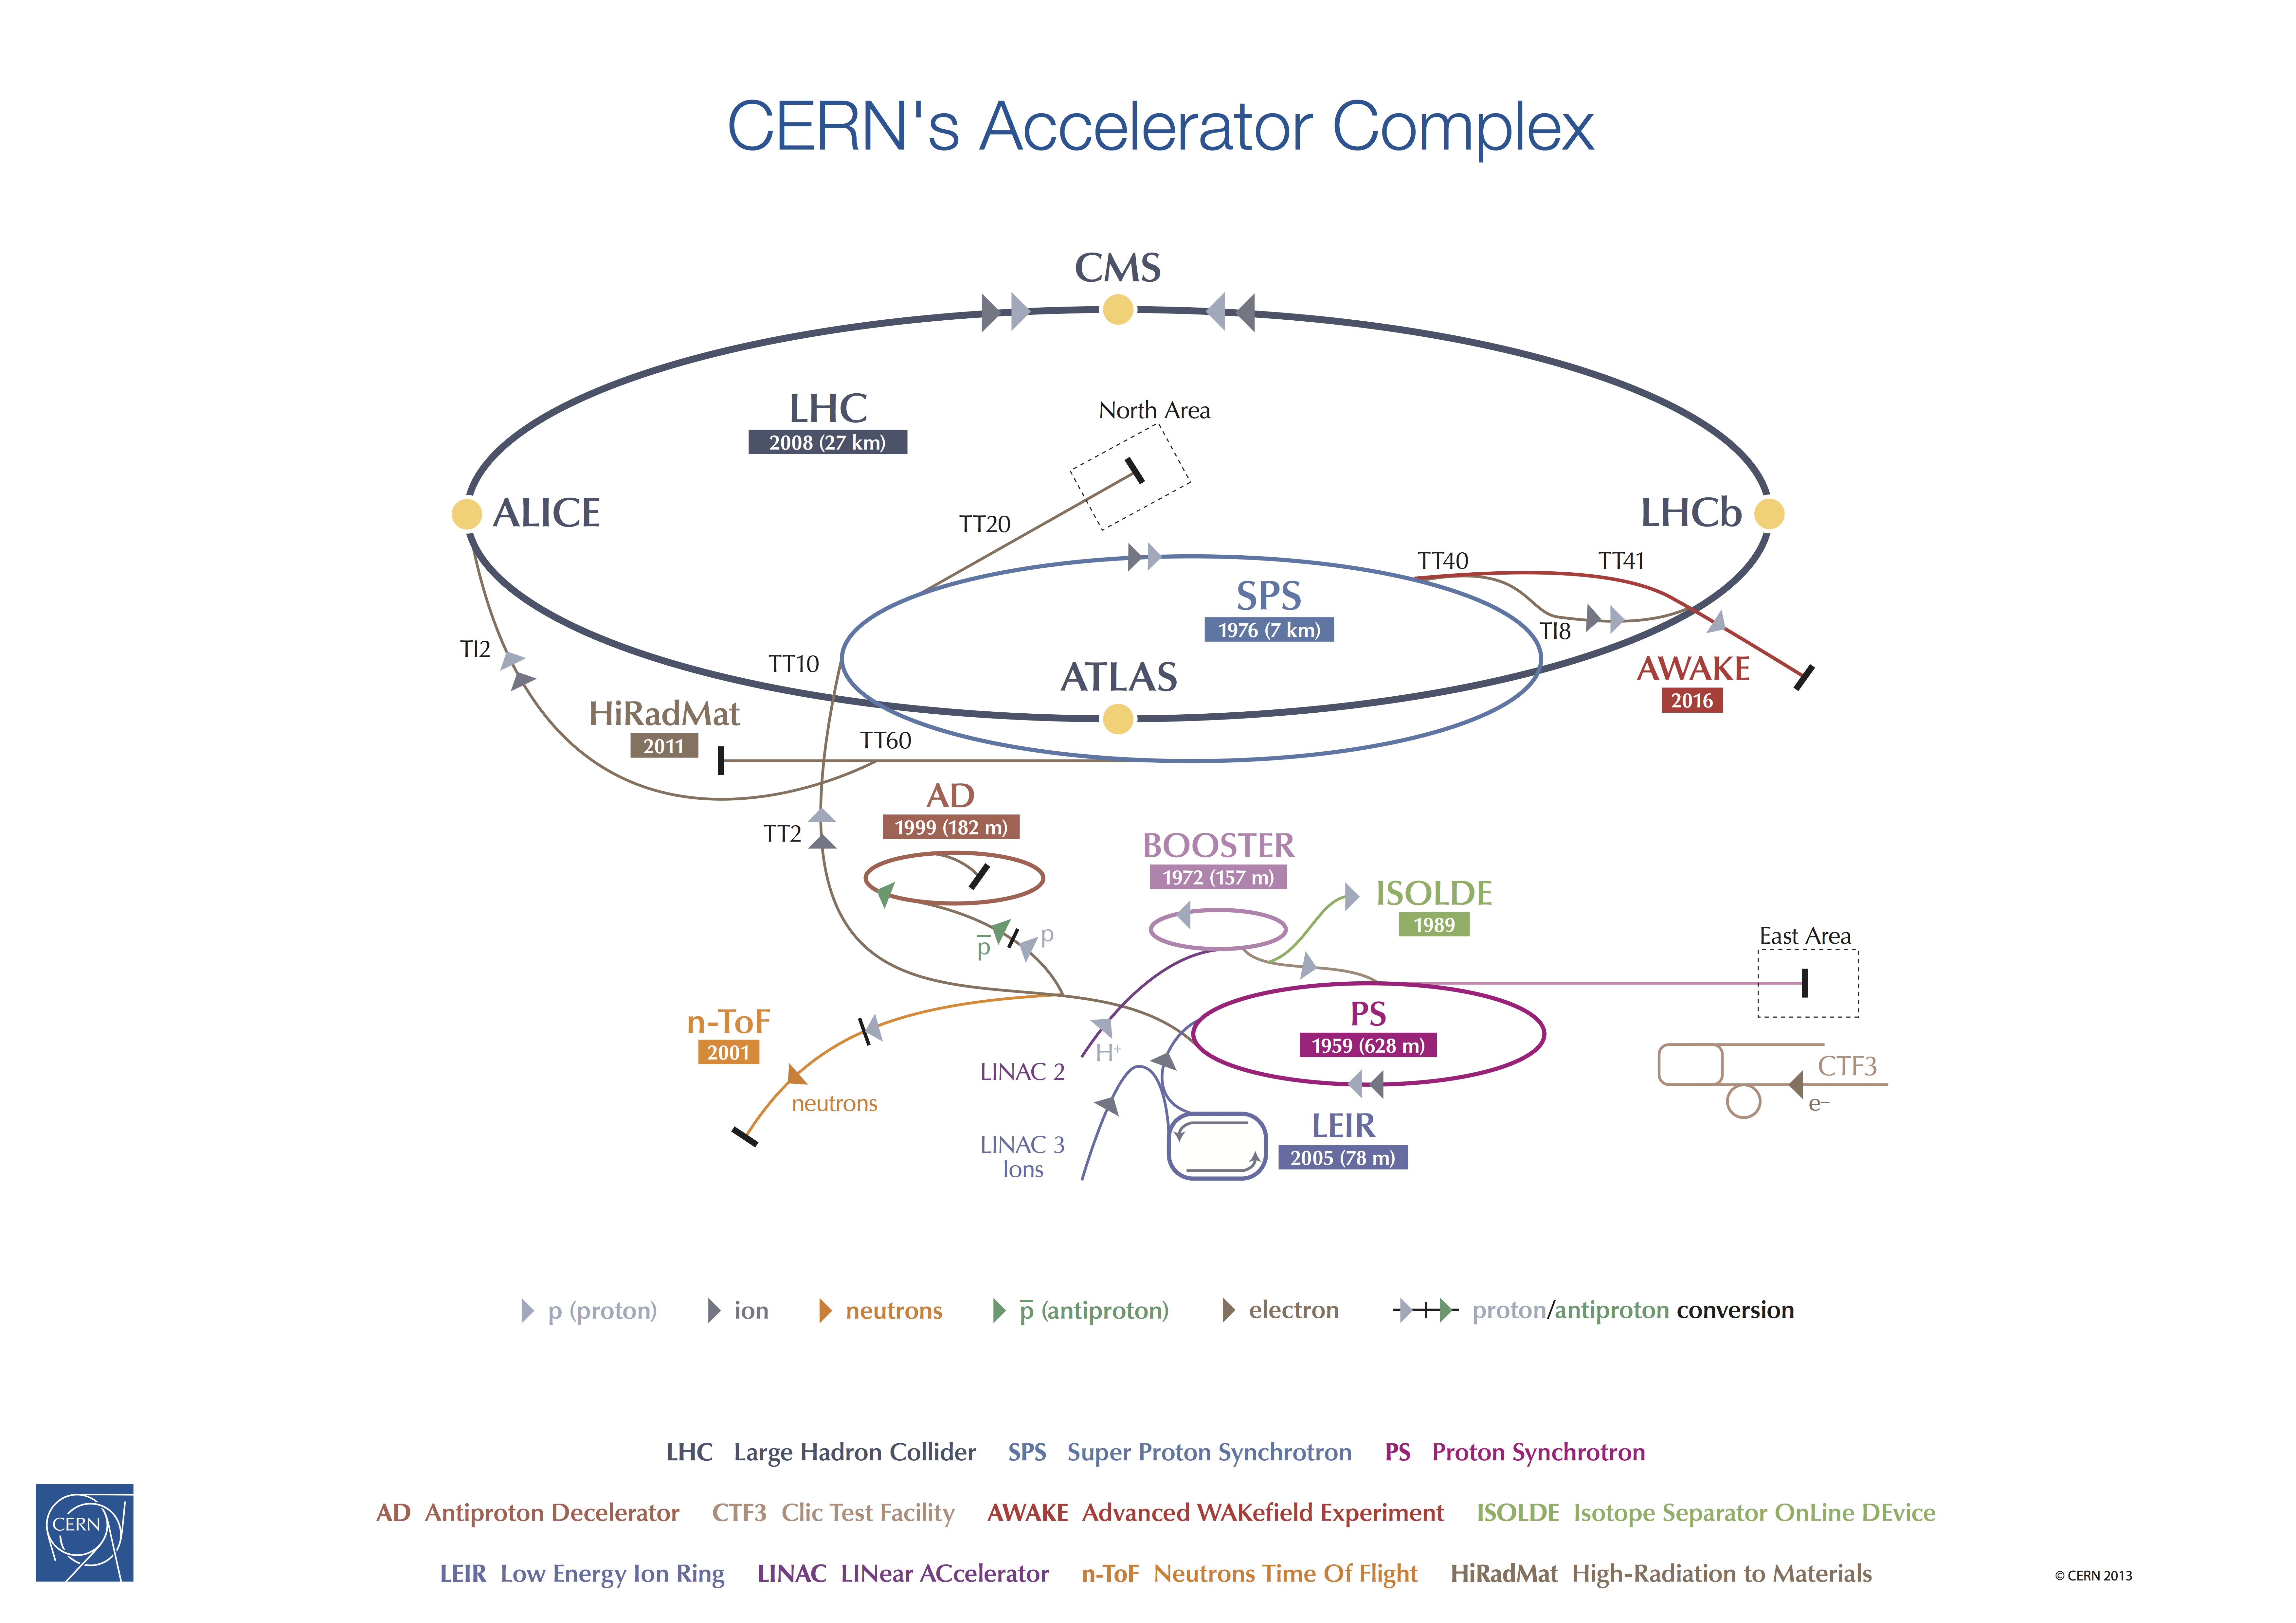
\includegraphics[width=18cm,height=10cm]{ch2/figures/CERN-Accelerator-Complex.jpg}
\caption{Picture showing the LHC ring and a series of accelerators which boost the proton (ion) beam to different energy levels~\cite{Web:CERN}.}
\label{fig:CERNAccComplex}
\end{figure}
Before two proton beams collide in the LHC at the desired center-of-mass energy, the beams have to be accelerated in several steps, as with the
presently available resources, it is experimentally challenging to reach an energy of 4\unit{TeV} (or designed 7\unit{TeV}) per beam in a single step.
Protons are first accumulated using hydrogen atoms contained in a simple bottle of hydrogen gas after stripping off electrons by applying an
electric field. Protons are then accelerated in \gls{LINAC2}, a linear accelerator consisting of RF cavities, to an energy of 50\unit{MeV}. These are 
then transferred to the Proton Synchrotron Booster (\gls{PSB}), which accelerates the beam to 1.4\unit{GeV}. Then the proton beams
are accelerated up to 25\unit{GeV} in the Proton Synchrotron (\gls{PS}) and up to 450\unit{GeV} in the Super Proton Synchrotron (\gls{SPS}). 
Finally, these are injected into the LHC rings and accelerated to an energy of 4\unit{TeV} resulting in a center-of-mass energy 
of 8\unit{TeV}. The entire CERN accelerator complex houses several experiments and facilities as illustrated in \fig{\ref{fig:CERNAccComplex}}.
Details of these can be found in Ref.~\cite{Web:CERN}. 

\begin{figure}[h!]
\centering
\includegraphics[width=10cm,height=8cm]{ch2/figures/lhcLayout_v2.png}
\caption{Layout of LHC ring~\cite{Web:CERNcds}.}
\label{fig:lhcLayout}
\end{figure}

The LHC tunnel is geometrically organized in eight crossing points, flanked by eight straight sections, and arcs. Each straight section has a 
length of 528\unit{m} and can serve as an experimental insertion, a point where two beams travelling in opposite directions can collide. A schematic 
representation of the LHC tunnel is depicted in \fig{\ref{fig:lhcLayout}}. The insertion points are labeled with 
integer numbers increasing in counter-clockwise direction. The LHC hosts four major detectors. A Toroidal LHC ApparatuS (ATLAS)~\cite{atlasTDR} and 
Compact Muon Solenoid (CMS)~\cite{cmsTDR} are the two general purpose detectors situated at points 1 and 5 insertion regions respectively. At point 2 
and 8 lie respectively, the experiments, A Large Ion Collider Experiment (\gls{ALICE})~\cite{aliceTDR} and Large Hadron Collider beauty (\gls{LHCb})~\cite{lhcbTDR}.
These two points also serve as the injection system for both the beams, one for the beam in clockwise direction and other for the beam in the 
counter-clockwise direction. Point 3 and 7 houses the collimation system while point 4 has two resonant frequency (RF) cavity system, one for each 
beam. Collimation system involves efficient cleaning of the beam halo during the LHC beam cycle, which limits the beam lifetime~\cite{Assmann:569470}. 
Point 6 is used as beam dump, where the beams are vertically extracted from the machine using  horizontally deflecting kicker magnets and vertically
deflecting double steel septum\footnote{Septum magnets are modified Lambertson-type septa with an all welded construction. More details about these 
can be found in Ref.~\cite{Evans:2008zzb}} magnets.

The LHC is designed to reach a center-of-mass energy up to 14\unit{TeV}. For any physics process the number of events generated by LHC
collision is given by
\begin{equation}
N = \mathcal{L}\sigma,
\end{equation}
where $\mathcal{L}$ is the instantaneous machine luminosity and $\sigma$ is the production cross section for a specific process. 
Assuming a Gaussian distributed beam in the $x$-$y$ plane, the machine instantaneous luminosity depends on various beam parameters, given by,
\begin{equation}
\mathcal{L} = F\frac{N^{2}_{b}n_{b}f_{rev}\gamma_{r}}{4\pi\epsilon_{n}\beta^{\ast}}
\end{equation}
where $N_{b}$ is the number of particles in each bunch, $n_{b}$ is the number of colliding bunches for each beam, $f_{rev}$ is the revolution 
frequency, $\gamma_{r}$ is the relativistic gamma factor, $\epsilon_{n}$ is the normalized transverse beam emittance, defined as the smallest 
opening the beams can be squeezed through. A low emittance beam implies that the particles are confined to a very small phase space thus having
the likelihood of higher particle interaction. $\beta^{\ast}$ is referred as the distance from the focus point where the beam width is twice as 
much to that at the focus point. $F$ is the geometrical reduction factor due to the non-zero beam crossing angle at the interaction point (IP), and is 
defined as,
\begin{equation}
F = \left(1+\left(\frac{\theta_{c}\sigma_{z}}{2\sigma^{\ast}}\right)\right)
\end{equation}
where, $\theta_{c}$ is the crossing angle at the IP, $\sigma_{z}$ is the rms bunch length, and $\sigma^{\ast}$ is the transverse
rms beam size at the IP.

It takes the protons about $89\mu{s}$ to circulate once in the LHC beam pipe. The LHC ring can accommodate  a maximum of 2808 proton bunches with 
a spacing of 25\unit{ns} and the rms beam size  at the IP5 is $16.7\mu{m}$.  In 2012, the LHC operated with 1380 bunches spaced at 50\unit{ns} each 
and containing up to $1.7\times10^{11}$ protons at an energy of 4.0\unit{TeV}. The 2012 proton-proton (pp) collision parameters $\epsilon_{n}$, 
$\beta^{\ast}$ and $F$ at the CMS interaction point were 2.5\unit{\mu{m}}, 0.6\unit{m}, and 0.8, respectively, yielding a peak instantaneous 
luminosity of $7.7\times10^{33}\unit{cm^{-2}s^{-1}}$. These parameters were optimized to give a high instantaneous luminosity and a stable beam 
with a long life time. It was difficult to further increase the instantaneous luminosity beyond a certain point as maximum particle density per 
bunch is limited by the non-linear beam-beam interactions when the bunches of two beams collide with each other. Also, the mechanical aperture of the 
magnets limits the minimum value that $\beta^{\ast}$ can attain at the IPs and the maximum value crossing angle can take in the experimental 
interaction regions. During the 8\unit{TeV} run in 2012, the LHC delivered an integrated luminosity of 23.3\unit{\fbinv} of \pp collision data to 
the ATLAS and CMS experiments, of which 21.8\unit{\fbinv} were recorded\footnote{During data taking, at times a sub-detector goes into error state 
due to several reasons and the data taking has to be stopped to take the sub-detector out and start a new run. Such situations lead to losses in the 
recorded data when compared to the delivered data.} by the CMS detector and 19.7\unit{\fbinv} was certified to be good for the physics analysis. The 
time-evolution of the total integrated delivered and recorded luminosities, during the 8\unit{TeV} run, is illustrated in \fig{\ref{fig:CMSLumi}}. 
This thesis is based on 19.7\unit{\fbinv} of \pp data collected by CMS detector in 2012.
\begin{figure}[h!]
\centering
% \subfloat[]{\label{fig:Lumi7TeV}\includegraphics[width=8cm,height=7cm]{ch2/figures/Lumi_pp_2011.pdf}}
 \includegraphics[width=8cm,height=7cm]{ch2/figures/Lumi_pp_2012.pdf}
 \caption{Total integrated luminosity delivered to the CMS experiment for \pp collisions by the LHC during the 2012 run at \sqrteighttev$\,$~\cite{Web:CMSLumi}.}
\label{fig:CMSLumi}
\end{figure}
\section{The Compact Muon Solenoid}
The Compact Muon Solenoid (CMS) experiment~\cite{Chatrchyan:2008aa} consists of a multi purpose $4\pi$ steridian detector and is installed at 
point 5 of the LHC ring, near the village Cessy in France. 
%Each part of the name has certain meaning. ``Compact" is used to denote the dimension of the detector, due to the use of heavier iron in the 
%detector for the magnetic field and muon system. The size of the CMS detector, having a diameter of 15\unit{m} and a length of 28.7\unit{m} 
%is much smaller compared to that of ATLAS detector's diameter of 25\unit{m} and 44\unit{m} length. However, the CMS detector weighs 14\unit{kTon}
%compared to ATLAS detector's weight of 7\unit{kTon}. The word ``Muon" is used due to the excellent muon system of the detector. ``Solenoid" is 
%used because of the geometrical shape of its magnetic field. 

As mentioned in the previous section, the LHC is designed to collide proton beams at $\sqrt{s}=14\unit{TeV}$, with an instantaneous luminosity 
of $10^{34}\unit{cm^{-2}s^{-1}}$. The large \pp total cross section, high beam intensity and short bunch spacing pose very challenging
requirements on the detectors in terms of radiation tolerance, high granularity, time-resolution and online data reduction. The conceptual 
design of the CMS detector was geared towards the detection of the SM Higgs boson and search for new particles, which led to excellent 
reconstruction efficiencies and energy resolutions for electrons, muons, photons, and hadrons~\cite{cmsTDR}. The requirements for the CMS detector
to meet the goals of the LHC physics program, coping with the demanding environmental conditions can be summarized as follows:
\begin{itemize}
\item Good identification and momentum resolution of muons over a wide range of momenta in the barrel region ($\abs{\eta}<2.5$), and a good dimuon mass 
resolution ($\sim$ 1\% at $100\unit{GeV/c^{2}}$ ), and the ability to determine the charge of muons with $\pt < 1\unit{TeV/c}$.
\item A tracker system with an excellent charged particle momentum resolution and reconstruction efficiency. The pixel detector is placed close to the 
interaction region for efficient triggering and offline tagging of $\tau$'s and \bjets.
\item An electromagnetic calorimeter with a good energy resolution and a good mass resolution ($\sim$1\% at $100\unit{GeV/c^{2}}$)
for diphoton and dielectron final states. It was also designed to be efficient in $\pi^{0}$ rejection, and isolation of photons and leptons at high 
luminosities.
\item Good \met\footnote{\met is referred to as the missing transverse momentum and is defined in \sectn{~\ref{sec:coord}}} and dijet mass resolution, requiring hadron calorimeters with a hermetic geometric coverage and with fine lateral segmentation.
\end{itemize}

The design of the CMS detector is similar to the structure of an onion. It consists of several layers of detectors, each one specially designed and
optimized to measure and identify different classes of particles. The main feature of the CMS experiment is a 3.8\unit{T} superconducting solenoid
magnet. Within the field volume are the tracker system, electromagnetic calorimeter, and hadronic calorimeter. A muon detection system is placed
outside the field volume of the solenoidal magnetic field embedded inside iron yoke and having return field for muon momentum measurement. 
A schematic view of the detector system is shown in \fig{\ref{fig:cmsDetector}}. In the following sections, the different components of the CMS 
detector are described in detail.

\begin{figure}[h!]
\centering
\includegraphics[width=16cm,height=13cm]{ch2/figures/cmsDetector.png}
\caption{Sectional view of the CMS detector~\cite{Web:CERNcds}.}
\label{fig:cmsDetector}
\end{figure}

\subsection{Coordinate System}\label{sec:coord}
The CMS follows a right-handed coordinate system, with origin defined to be the nominal collision point at the center of the detector.
The $x-$axis points radially towards the center of the LHC ring, the $y-$axis vertically upwards while the $z-$axis points west, along the beam
direction towards the Jura Mountains from LHC point 5. The polar angle $\theta$ is measured from the $z-$axis, while the azimuthal angle 
$\phi$ is measured from the $x-$axis in the $x-y$ plane. The radial coordinate, $r$, is defined in the $x-y$ plane. Instead of $\theta$, it is 
often more handy to use rapidity $y$, defined as:
\begin{equation}
y = \frac{1}{2}\ln\left(\frac{E+p_{z}}{E-p_{z}}\right),
\end{equation}
where $E$ and $p_{z}$ are the measured energy and $z-$ component of the momentum carried by the particle. The key reason why rapidity is a crucial 
quantity is because the rapidity differences are invariant with respect to Lorentz boost along the beam axis. But another quantity, known as 
pseudorapidity and defined as:
\begin{equation}
\eta=-ln\left[\mathrm{tan}\left(\frac{\theta}{2}\right)\right],
\end{equation}
is preferred at the hadron colliders. For highly relativistic particles the two quantities are almost identical, $y\simeq\eta$. The rapidity
in terms of pseudorapidity is given by
\begin{equation}
y = ln\left( \frac{\sqrt{m^{2} + \pt^{2}\text{cosh}^{2}\eta} +\pt\text{sinh}\eta}{\sqrt{m^{2} + \pt^{2}}}\right).
\end{equation}
%The only issue with rapidity is that it can be difficult to measure this quantity for highly relativistic particles as it requires both the energy 
%and the total momentum of the particle and in reality it is difficult to get the total momentum of a particle, especially at high values of the 
%rapidity where the $z-$component of the momentum is large, and the beam pipe can be in the way of measuring it precisely. 
The angular separation of two events, ($y_{2}-y_{1}$, $\phi_{2}-\phi_{1}$) is invariant with respect to boosts along the beam axis
and the angular distance between two objects, as observed from the origin of the CMS detector, is expressed as:
\begin{equation}
R = \sqrt{(\deta)^{2}+(\dphi)^{2}}.
\end{equation}
In collider experiments, the incoming particles collide head-on and have no transverse momentum before scattering and therefore by momemtum 
conservation, the final state particles must have zero total transverse momentum. Hence, the momentum and energy of the object are measured 
transverse to the beam direction, denoted by \pt and \et, respectively, where $\pt = \sqrt{p_{x}^{2} + p_{y}^{2}}$ and $\et = E\,\text{Sin}\theta$.
The missing transverse momentum is defined as the negative vector sum of all particles detected by the detector, $\metVec\equiv -\sum \vec{\pt}$.
Momentum conservation dictates that \metVec is equal, in the limit of a perfect detector efficiency and resolution, to the vector sum of transverse 
momentum of all undetected particles such as neutrinos or some new particle and the energy lost in nuclear processes.

\subsection{Magnet}
The choice of the magnet is crucial for ensuring good performance for a high energy physics experiment. Precise measurement of the charged
particle momenta at a wide range of energies requires high bending power that can be achieved using strong magnetic field. For a charged
particle in a uniform magnetic field, B, the momentum of the particle is given by, $p=\gamma{mv}=qBr$, where $q$ is its charge, $m$ is its
mass and $r$ is the bending radius of the particle. The trajectory of a charged particle in the magnetic field is an arc of radius $r$ and path 
length $L$. The sagitta of the trajectory, defined as the perpendicular distance from the midpoint of the arc's chord to the arc itself and is given 
by $s = \frac{L^{2}}{8r} = \frac{qBL^{2}}{8p}$. Assuming that the particle crosses the full solenoid, $L$ is equal to the radius of the solenoid.
The \pt resolution depends on the magnetic field and solenoid radius as, $\frac{dp}{p}\propto\frac{p}{BL^{2}}$.

Therefore, for improvement in the resolution both a large size and a strong magnetic field is needed. The CMS design~\cite{cmsMagnet} having a 
solenoid of 6\unit{m} in diameter (and also a large tracker that defines the measurable path length) and a strong magnetic field of 3.8\unit{T} meets 
the requirement.

The CMS magnet~\cite{cmsMagnet} consists of two main parts, the coil and the yoke. The coil forms the superconducting solenoid which utilizes a 
4-layer winding made from a stabilized reinforced NbTi conductor to give a magnetic field of 3.8\unit{T}. The yoke comprised of 11 large elements, 
5 barrel wheels and 6 endcap disks, that returns magnetic flux yielding a field of about 2\unit{T}. The yoke was designed to achieve a balance
between the outer diameter of the yoke and the size of the muon system\footnote{Muon system is described in more detail in \sectn{\ref{sec:muon}}}~\cite{Chatrchyan:2008aa}. At full current, the energy stored in the
magnetic field is $\sim2.7\unit{GJ}$.

\subsection{Tracking System}
The tracker is the innermost sub-system of the CMS detector. It is designed to measure precisely and efficiently the trajectories of charged 
particles from the interaction point, and reconstruct both primary and secondary vertices. It not only reconstructs the paths of muons, 
electrons, and charged hadrons, but also the tracks coming from the decay of very short-lived particles such as $b-$ and $c-$quarks, with high momentum resolution and efficiency.
\begin{figure}[h!]
\centering
%\includegraphics[width=14cm,height=7cm]{ch2/figures/TrackerLayoutNew.pdf}
\includegraphics[width=14cm,height=7cm]{ch2/figures/TrackerLayout.png}
\caption{ Schematic view of the CMS tracker in the $r-z$ plane~\cite{Chatrchyan:2008aa}. Each line depicts a detector module and double lines represents back-to-back modules. Abbreviations TEC, TIB, TID, TOB, etc. are described later in text.}
\label{fig:trackerLayout}
\end{figure}

A tracker system~\cite{Chatrchyan:2008aa,Karimaki:368412} covering the region $\abs{\eta}<2.5$ and employing more than 200\unit{m^2} of active Si 
sensors is shown in \fig{\ref{fig:trackerLayout}}. It surrounds the interaction point and has a length of 5.8\unit{m} and a diameter of 2.5\unit{m}. 
The CMS solenoid provides a homogeneous magnetic field of 3.8\unit{T} over the full volume of the tracker. At high luminosity, 20 overlapping \pp 
collisions at the LHC would, on an average, result in 1000 particles traversing the tracker for every bunch crossing, \ie every 25\unit{ns}. Therefore, 
a detector featuring high granularity and fast response is needed to cope with the large levels of occupancy and radiation. In addition, the intense 
particle flux will also cause severe radiation damage to the tracking system. These requirements on granularity, speed and radiation hardness 
necessitate a tracker design based entirely on silicon detector technology.

The tracks in the CMS are seeded by the hits in the tracker detector. The compatible hits are added to update the trajectory 
until either the detector boundary is reached, or no additional compatible hits\footnote{Hits compatible with the extrapolation of parameters
for a track, growing trajectory of a track, and their covariance matrix in the detector material.} can be found. The collection of hits is then
used to obtain the best estimate of the track parameters. However, the large amount of material within the tracker volume affects the overall
event topology and reconstruction due to electron bremsstrahlung, conversions of photons to electron pairs and nuclear interactions.
Therefore, it is important to estimate the amount of material of the CMS tracker. This is shown in \fig{\ref{fig:MaterialBudget}} --- both in 
%\fig{\ref{fig:MaterialBudget}} is taken from link~\cite{Chatrchyan:2014fea}
\begin{figure}[h!]
\centering
 \subfloat[]{\includegraphics[width=7.6cm,height=7cm]{ch2/figures/MaterialBudget_RadLengths.pdf}}
\hspace{0.5cm}
 \subfloat[]{\includegraphics[width=7.6cm,height=7cm]{ch2/figures/MaterialBudget_InteractionLengths.pdf}} 
 \caption{Total thickness of the tracker material traversed by a particle produced at the nominal interaction point, as a function of pseudorapidity, expressed in units of (a) radiation length $\mathrm{X_0}$ and (b) nuclear interaction length $\lambda_I$~\cite{Chatrchyan:2014fea}.}
\label{fig:MaterialBudget}
\end{figure}
units of radiation length ($\mathrm{X_0}$) and nuclear interaction length ($\lambda_I$) as a function of pseudorapidity, as estimated from simulation 
within about$\sim10\%$ accuracy~\cite{Karimaki:368412,CMS:2010nua,Chatrchyan:2014fea}. The $\mathrm{X_0}$ corresponds to the mean distance over 
which an electron loses a fraction 1/e of its energy. It also corresponds to 7/9 of the mean free path for pair production of a photon. At $\eta=0$, 
the tracker material budget corresponds to about 0.4\unit{X_0}, while at the boundary between the barrel and the endcaps, the material budget reaches 
a value of 1.8\unit{X_0} due to cabling and other services like mechanical support in this region. The CMS tracker is composed of a pixel detector 
and a silicon strip tracker which are described in details in the sections to follow. 

\subsubsection{Pixel Detector}
The pixel detector~\cite{Chatrchyan:2008aa,Karimaki:368412} is the part of the tracking system closest to the interaction region with a
 pseudorapidity coverage of $\abs{\eta}<2.5$, as shown in \fig{\ref{fig:pixelDetector}}. Being very close to the interaction 
vertex and beam direction, it is inundated with a very large particle flux. It contains about 66\unit{million} Si pixels, allowing it to provide 
precise and highly accurate tracking points in three dimensional space, ($r$, $\phi$ and $z$) for all emerging particles. This is essential for 
reconstruction of secondary vertex from decays of \bquark and tau leptons and forming seed tracks for the reconstruction of outer tracks. The pixel 
cells, of size 100$\times$150\unit{\mu{m}^{2}}, are used to attain an occupancy level of $\sim 10^{-1}$/(pixel$\times$bunch-crossing). 
The pixel has a zero-suppressed analog pulse height read-out scheme that improves position resolution and helps in separating signal from noise hits 
as well as identifying large hit clusters from overlapping tracks. 
\begin{figure}[h!]
\centering
 \subfloat[]{\includegraphics[width=6cm,height=5cm]{ch2/figures/PixelLayout.png}}
\hspace{1cm}
 \subfloat[]{\includegraphics[width=7cm,height=6cm]{ch2/figures/pixelDetector.png}} 
 \caption{(a) Hit coverage and (b) geometrical layout of the CMS pixel detector~\cite{Chatrchyan:2008aa}.}
\label{fig:pixelDetector}
\end{figure}

The layout of the pixel system consists of three barrel layers (\gls{BPIX}) with two endcap disks (\gls{FPIX}). The 53\unit{cm} long BPIX 
layers are located at mean radii of 4.4, 7.3 and 10.2\unit{cm}, whereas the FPIX extends from 6 to 15\unit{cm} in radius and are placed at 34.5 and 
46.5\unit{cm} on both sides of the nominal interaction point. The BPIX (FPIX) layers contain 48\unit{million} (18\unit{million}) pixels covering a 
total area of 0.78 (0.28)\unit{m^2}. The forward detectors are tilted at 20$^{\circ}$ in a turbine-like geometry to induce charge 
sharing~\cite{Atac:2002mk}. The pixel detector has a spatial resolution in the range of $15-20\unit{\mu{m}}$~\cite{Karimaki:368412}.
Unfortunately, they would need to be replaced during the time period of the experiment, due to radiation damage.



\subsubsection{Silicon Strip Detectors}
The silicon strip tracker~\cite{Chatrchyan:2008aa,Karimaki:368412} is composed of 15148 detector modules distributed among the four different 
subsystems $-$ Tracker Inner Barrels (\gls{TIB}), Tracker Inner Disks (\gls{TID}), Tracker Outer Barrels (\gls{TOB}) and Tracker EndCaps (\gls{TEC}). Each module
carries either one thin (320\unit{\mu{m}}) or two thick (500\unit{\mu{m}}) silicon sensors. The dimension of the strips increases with increasing 
distance from the interaction point so that the occupancy level is kept to $\sim1\%$. The occupancy is defined as the number of strip measurements 
in an event divided by the number of all active strips. The silicon detectors work in much the same way as the pixels $-$ a charged particle crosses 
the material, knocks out electrons from the atom and within the applied electric field, gives a very small pulse of current lasting a few nanoseconds. 
The schematic longitudinal view of the silicon strips in terms of different layers and their arrangements in $\eta$ and $z$ plane is shown in 
\fig{\ref{fig:SiliconStrips}} .
\begin{figure}[h!]
 \centering
 \includegraphics[width=12cm,height=6cm]{ch2/figures/SiliconStrip.png}
 \caption{A Schematic layout of the silicon microstrip detector~\cite{Chatrchyan:2008aa}.}
 \label{fig:SiliconStrips}
\end{figure}

The TIB and TID are composed of four barrel layers and three disks at each end. The silicon strip tracker provides up to four $r-\phi$ measurements 
with a position resolution of 23\unit{\mu{m}} in the two inner layers and 35\unit{\mu{m}} in the two outer layers~\cite{Chatrchyan:2008aa}. The TIB 
and TID are surrounded by the six layers of TOB, providing a resolution of 53\unit{\mu{m}} in the first four layers and 35\unit{\mu{m}} for the outer 
two layers~\cite{Chatrchyan:2008aa}. Beyond $z=118\unit{cm}$ TEC provides additional forward coverage up to $\abs{\eta}<2.5$, giving nine $\phi$ 
measurements per trajectory and extending up to 282\unit{cm}~\cite{Chatrchyan:2008aa}.

\subsection{Calorimeter System}
A calorimeter is a detector which measures the energy of a particle. The CMS calorimeters are designed to measure the energy of electrons, photons 
and hadrons (jets) produced in collisions. The CMS calorimeter is divided into electromagnetic and hadronic sections. The electromagnetic calorimeter 
(\gls{ECAL}) is used to measure the energy of particles which interact electromagnetically such as photons and electrons whereas the hadronic calorimeter 
(\gls{HCAL}) is designed to measure the energy of strongly interacting particles. Hadrons interact via strong force leading to showers that has both 
electromagnetic and hadronic component. The hadronic component of the shower scales with the nuclear interaction length and can not be contained 
within the ECAL. Muons, though interact via electromagnetic force, behave in a very different way. They loose energy primarily through ionization,
with energy losses of the order of $1-2$\unit{MeV/g/cm^{2}} and, therefore, different sub-system is needed for the detection of muons. 
Interacting with matter via the weak force, neutrinos typically pass through the matter unimpeded and undetected, and can be observed only indirectly 
as an imbalance in event energy in the transverse plane. The measurement of this imbalance, termed as missing transverse energy, plays a critical 
role for new physics searches, such as compositeness, supersymmetry, extra dimensions etc.

\subsubsection{Electromagnetic Calorimeter}
The ECAL~\cite{Chatrchyan:2008aa,ecalTDR} is a homogeneous, hermetic calorimeter made up of 61200 lead tungstate (PbWO$_4$) scintillating crystals 
mounted in the central barrel part, accompanied by 7324 crystals in each of the two endcaps. It covers the pseudorapidity region up to
$\abs{\eta}<3$, and is complemented, in the forward region ($1.653<\abs{\eta}<3.0$) by Si-Pb preshower, as shown in \fig{\ref{fig:Ecal}}. In order 
to fulfill the scientific goals of the CMS, the ECAL was designed to have a high energy resolution for e/$\gamma$ objects. To achieve this, the ECAL 
was positioned inside the CMS magnet so that the amount of energy loss due to the material upstream can be minimized. 
\begin{figure}[h!]
 \centering
 \includegraphics[width=13cm,height=8cm]{ch2/figures/cmsECAL.png}
 \caption{A schematic design of the CMS ECAL showing the arrangement of crystals, supermodules and endcaps with the preshower in front~\cite{Chatrchyan:2008aa}.}
 \label{fig:Ecal}
\end{figure}
Within the LHC environment, it is important to design a calorimeter which is fast, has fine granularity and is radiation tolerant. 
The PbWO$_4$ crystals have a large density (8.28\unit{g}/cm$^{3}$), a small radiation length X$_{0}$ (0.89\unit{cm}), and a small Moli\'{e}re 
radius (2.2\unit{cm}), which makes them an appropriate choice for a compact and high granular calorimeter. The total amount of material between the 
interaction point and the ECAL increases from 0.4\unit{X_0} close to $\eta=0$ to almost 2\unit{X_0} near $\abs{\eta}=1.4$, before falling 
again to about 1.3\unit{X_0} around $\abs{\eta}=2.5$. Therefore, the resolution of the ECAL depends on the \pt and $\eta$ of the object,
and whether the electron or photon undergoes bremsstrahlung.

The ECAL barrel (\gls{EB}) covers the region $\abs{\eta}<1.48$, and has an internal surface radius of 1290\unit{mm}. It is made up of 61,200 
trapezoidal crystals. Each crystal has a frontal area of approximately $22\times22\unit{mm^{2}}$ and a length of 230\unit{mm} (25.8\unit{X_{0}}),
which leads to a granularity of 0.0174 in $\eta$ and $\phi$. A half-barrel consist of 18 supermodules, each containing 1700 crystals and covering
$20^{\circ}$ in $\phi$. Photodetectors are placed in front of the crystals to collect the light and convert it into signals which can be read out 
by the electronics chain. Since the light yield from the PbWO$_{4}$ crystals is relatively low, amplification of the signal needs to be done, and 
hence silicon avalanche photodiodes (\gls{APDs}) are used. In addition to intrinsic gain, APDs are also insensitive to magnetic fields and have high 
radiation resistance and are, thus, suitable for EB.

The endcaps (\gls{EE}) cover the region $1.48<\abs{\eta}<3.00$, are located at $\abs{z}>3154\unit{mm}$ and are composed of 4 half disks. Each half-disk 
is made up of 3,662 trapezoidal crystals each having a frontal area of $28.6\times28.6\unit{mm^{2}}$ and a length of 220\unit{mm} 
(24.7\unit{X_{0}}). The crystals in each disk are organized into 138 standard $5\times5$ supercrystal units with 52\unit{mm} wide voids in between 
the groups. The crystals are arranged in a quasi-projective geometry pointing $\pm1300\unit{mm}$ beyond the nominal  interaction point. 
Photodetectors used in the EE are Vacuum phototriodes (\gls{VPTs}). The VPTs can be operated in a very high radiation environment and hence are used in the EE.

A preshower detector is a pair of sampling calorimeters designed to distinguish neutral pions from real photons and improves the position
measurement of electrons and photons with high granularity. Each calorimeter consists of two planes of silicon sensors interleaved with 
a total of 3\unit{X_{0}} of lead and is located in front of the EE and covers the region $1.65<\abs{\eta}<2.60$.

The ECAL energy resolution for electromagnetic showers below 500\unit{GeV}, can be parametrized as :
\begin{equation}
\left(\frac{\sigma}{E}\right)^{2} = \left(\frac{S}{\sqrt{E}}\right)^{2} + \left(\frac{N}{E}\right)^{2} + C
\end{equation}
where $S$ is the intrinsic stochastic term, $N$ is the noise term and $C$ is the constant term with details as follows :
\begin{itemize}
\item Stochastic term ($S$) : This includes contribution from event-to-event fluctuation in the lateral shower containment, photostatistics
contribution, fluctuations in the energy deposited in the preshower absorber (where present) with respect to what is measured in the 
preshower silicon detector. The contribution of these fluctuations to the energy resolution of the calorimeters follow Poissonian distribution,
hence the resolution scales as $1/\sqrt{E}$.
\item Noise term ($N$) : The three contributions to the noise term include : electronics noise; digitization noise; and pileup noise. The signal 
amplitude in the test beam is reconstructed using a simple digital filter. The noise measured, after this amplitude reconstruction, for 
channels in barrel supermodules is $\sim40\unit{MeV}$/channel in the highest gain range. This noise includes both electronics and 
digitization noise and varies as $1/E$. The noise from the pileup is found to be very small.
\item Constant term ($C$): The most important contributions to the constant term include: non-uniformity of the longitudinal light collection,
 inter calibration errors, and leakage of energy from the back of the crystal. %The constant term can be reduced by utilizing radiation hard media and
% performing in-situ calibration. The CMS calorimeter accounts for both the factors by utilizing a laser monitoring and a calibration system
\end{itemize}
The test beam results~\cite{Chatrchyan:2008aa,CMS:2010zta} using the energy measurement in $3\times3$ crystal lattice, lead to the following values 
for the various terms : $S=2.8\%$, $N=124\unit{MeV}$, and $C=0.3\%$ in the barrel regions and $S=5\%$, $N=500\unit{MeV}$ and $C=0.3\%$ for the 
endcap regions.

\subsubsection{Hadronic Calorimeter}
The hadronic calorimeter~\cite{Chatrchyan:2008aa,hcalTDR} is a sampling calorimeter surrounding the ECAL, which is used in conjunction with 
the ECAL to measure the energy and direction of hadronic particles and to estimate the missing transverse momentum (\met).
%The determination of missing energy and jets are crucial for new particles and phenomena, such as supersymmetric partners of 
%quarks and gluons. Indirectly, the HCAL also helps in the identification of electrons and photons. 
The HCAL is composed of four sub-detectors $-$ HCAL Barrel (\gls{HB})~\cite{Abdullin:2008zzb}, HCAL Endcaps (\gls{HE})~\cite{Baiatian:2008zz}, 
HCAL Outer (\gls{HO})~\cite{Abdullin:2008zza}, and HCAL Forward (\gls{HF})~\cite{Bayatian:2006jz} as shown in \fig{\ref{fig:cmsHCAL}}. 
The HCAL consists of plastic scintillator tiles read out with embedded wavelength-shifting (\gls{WLS}) fibres interleaved with overlapping brass plates 
for the absorber material.
\begin{figure}[h!]
 \centering
 \includegraphics[width=13cm,height=8cm]{ch2/figures/cmsHCAL.png}
 \caption{A schematic design of the CMS HCAL showing the barrel section (HB), endcap section (HE), the tail catcher outside the solenoid (HO) and the forward section (HF)~\cite{cmsTDR}.}
 \label{fig:cmsHCAL}
\end{figure}

The HB detector consists of 36 identical azimuthal wedges covering the region $\abs{\eta}<1.3$. Each wedge is segmented into 16
azimuthal plates, bolted together in such a way that there is no projective dead material. The absorber is made of brass (70\% Cu
and 30\% Zn), except for the first and last layers which are made of stainless steel for structural strength. It is restricted 
between the outer extent of the ECAL ($R=1.77\unit{m}$) and the inner extent of the magnet ($R=2.95\unit{m}$), which constrains
the total amount of material that can be put in to absorb the hadronic shower. Therefore, to ensure adequate sampling of the
hadronic showers, the calorimeter was extended outside of the solenoid  with a tail catcher called HO, which uses the solenoid 
as an additional absorber layer. The total thickness of the calorimeter system is thus extended to a minimum of 11.8$\lambda_{I}$. 
The HE covers the region $1.3<\abs{\eta}<3.0$. The active medium uses the tile and wavelength shifting fibre concept to bring out 
the light, which is then read out by means of hybrid photo diodes (\gls{HPDs}). Up to $\abs{\eta}<1.6$, the HCAL towers have a size of 
$\Delta\eta\times\Delta\phi=0.087\times0.087$, while for $\abs{\eta}>1.6$, the size increases to $\Delta\eta\times\Delta\phi\sim0.175\times0.175$.

To cope with the exceptionally high radiation dose (up to about 10\unit{mSv}/h), the HF calorimeters (located only 11\unit{m} away from
the interaction point) covering the region $3.0<\abs{\eta}<5.0$ uses more robust, minimal-maintenance quartz fibres as the active material 
and steel as the absorber material. The HF is designed to improve the measurement of \met and to enable identification and reconstruction of 
very forward jets which constitute distinguishing characteristics of several important physics processes. A signal is generated in the HF when 
a charged particle traverses a quartz fiber with a velocity greater than speed of light in the fiber, resulting in Cherenkov radiation.

%The energy resolution of the HCAL, in contrast to that of the ECAL, is limited due to the nature of the hadronic interactions. During a hadronic
%interaction, a part of the energy is purely electromagnetic due to the presence of $\pi^{0}$ and $\eta$ mesons decaying to photon pairs
%and is thus measured directly by photodetectors. Charged particles, on the other hand produce signal by ionization, excitation and nuclear
%interactions. In most of the cases, a significant fraction of the energy (of the order of 20-35\%), deposited in a sampling calorimeter
%is not visible resulting in a degraded resolution. 
For the CMS HCAL, the resolution is parametrized as~\cite{cmsTDR,Leonard:2010zda} :
\begin{equation}
\left(\frac{\sigma}{E}\right)^{2} = \left(\frac{A}{\sqrt{E}}\right)^{2} + \left(B\right)^{2},
\end{equation}
with the parameters, for both HB~\cite{Abdullin:2008zzb} and HE~\cite{Baiatian:2008zz}, being $A=0.847\unit{GeV}$ and $B=0.074$. 
Corresponding values for the HF~\cite{Bayatian:2006jz} are $A=1.98\unit{GeV}$ and $B=0.09$.

The CMS calorimeter system is non-compensating, \ie its response to electrons is not same as to that to hadrons of the same energy.
Experimentally, the $e/h$ ratio is not directly accessible. Instead, the ratio of the responses to pion and electron ($\pi/e$) was measured in 
test beams~\cite{Abdullin:2009zz} and is related to the $e/h$ ratio by the formula :
\begin{equation}
\frac{e}{h} =\frac{1-f_{em}}{\pi/e - f_{em}},
\end{equation}
where $f_{em}$ is the electromagnetic fraction of the shower energy. For test beam particles with energies above $\sim8\unit{GeV}$, the $h/e$ ratio
was found to be $1.4\pm0.1$. An event-by-event correction scheme was developed~\cite{Abdullin:2009zz,Wigmans:2010zz}. A linear response 
(within 1.3\%) to hadrons of momenta between 5 and 350\unit{GeV} was achieved. 


\subsection{Muon System}\label{sec:muon}
The muon system~\cite{muonTDR} forms the last component of the CMS detector following the super conducting solenoid. 
%Because of their high mass and longer lifetime, muons provide the cleanest experimentally measurable signatures. 
The CMS has been designed to provide good muon identification, momentum resolution and efficient trigger on muons within $\abs{\eta}<2.4$ and $\pt\le1\unit{TeV}$.

The muon system uses three different technologies to detect muons: drift tubes (\gls{DT}) in the barrel 
region ($\abs{\eta}<1.2$), cathode strip chambers (\gls{CSC}) in the endcap region ($\abs{\eta}>1.2$) and resistive plate chambers (\gls{RPC}) in both, 
the barrel and the endcaps. The RPCs provide a lower spatial resolution but a faster response than the DTs or CSCs. The DTs/CSCs and the 
RPCs provide two independent and complementary sources of information for the first level trigger\footnote{More detail about trigger system is given
in \sectn{\ref{Se:triDas}}} to ensure a robust, flexible and precise trigger 
decision. A diagram showing the mechanical layout of the three muon detection systems can be found in \fig{\ref{fig:cmsMuonSystem}}.
\begin{figure}[h!]
 \centering
 \includegraphics[width=13cm,height=8cm]{ch2/figures/cmsMuonSystem.png}
 \caption{A schematic design of one quadrant of the muon system in the $r-z$ plane showing the position of three sub-detectors used for muon detection~\cite{Web:CERNcds}.}
 \label{fig:cmsMuonSystem}
\end{figure}

\subsubsection{Drift Tube Chambers}
In the barrel region, where the muon flux is low and the magnetic field uniform, four layers of muon stations are used, occupied by drift tube (DT) 
chambers covering up to $\abs{\eta}<1.2$. The three innermost stations are comprised of 12 chambers each, which measure muon coordinates in the $r-\phi$ plane and provide a measurement in the $z-$direction, while the outermost station measures only the 
$\phi-$view. The DT chambers 
consist of individual drift tube cells that contain a 50\unit{\mu{m}} diameter anode wire and two electrode plates that
 create the drift electric field. The walls of the cell are grounded, acting as cathodes. 
%The drift cells of each chamber are 
%offset by a half-cell width with respect to their neighbors so as to eliminate dead spots in the efficiency. 
The cells are filled with a gas mixture (85\% Ar and 15\% CO$_{2}$) and the wire and electrodes are operated with a voltage difference of 
about 1.8\unit{kV}. The transverse dimension of the cells was chosen to be 21\unit{mm} to optimize drift time, gain and number of channels. 
With these design parameters, the DT achieve a gain of 10$^{5}$, resulting in a drift time of 380\unit{ns} and a linear relationship between 
drift time and drift path which is essential for the chamber to provide triggering capabilities. \Fig{\ref{fig:cmsDT}} shows the basic design 
of a DT cell. 

\begin{figure}[h!]
 \centering
 \includegraphics[width=13cm,height=8cm]{ch2/figures/DT.jpg}
 \caption{Individual drift tube cells and pictorial representation of its operation principle~\cite{cmsTDR}.}
 \label{fig:cmsDT}
\end{figure}

\subsubsection{Cathode Strip Chambers}
In the endcap regions, where the magnetic field is large and non-uniform, cathode strip chambers (CSC) are installed providing a coverage in the 
region $0.9<\abs{\eta}<2.4$. The CSCs are multi-wire proportional chambers consisting of six planes of anode wires interleaved among seven cathode 
panels. The gold-plated tungsten wires run azimuthally, defining the track's radial component, while the strips are milled on cathode panels and run 
lengthwise at a constant \dphi width. The angular ($\phi$) position of the track is estimated by extrapolating the charge that is induced on the 
strips as shown in \fig{\ref{fig:cmsCSC}}. The nominal gas mixture is 40\% Ar, 50\% CO$_{2}$ and and 10\% CF$_{4}$. Addition of CF$_{4}$ helps to 
avoid polymerization on wires. The wires give very fast signals that provide very good time resolution while the development of the avalanche on 
the strips gives very good position resolution. The CSCs can operate at high rates and in large and non-uniform magnetic fields without requiring 
precise monitoring of gas, pressure or temperature and can provide trigger and precision position measurement in the same device. The CSC system 
comprises of 468 trapezoidal chambers covering 10$^{^{\circ}}$ or 20$^{^{\circ}}$ in the $\phi-$direction.
\begin{figure}[h!]
 \centering
 \includegraphics[width=13cm,height=8cm]{ch2/figures/csc.png}
 \caption{Operation principle of the Cathode Strip Chamber~\cite{Web:CERNcds}.}
 \label{fig:cmsCSC}
\end{figure}

\subsubsection{Resistive Plate Chambers}
In order to improve the performance of the muon trigger, an additional system of resistive plate chambers (RPCs) is installed, spanning both the 
barrel and the endcap regions. The RPC system has 480 barrel and 432 endcap chambers. Two rectangular section RPCs per DT chamber are installed 
in the barrel region and two trapezoidal ones per CSC chambers are installed in the endcap regions. They are parallel plate gaseous detectors that 
combine adequate position resolution with a very high operational speed. The RPC is able to tag the presence of an ionizing particle in a time-frame
much shorter than the typical bunch crossing time, which makes it an ideal trigger device since, together, they can associate the correct bunch 
crossing (25\unit{ns} between two bunch crossings) with the muon. The CMS RPC chamber consists of two gaps operated in an avalanche mode with read-out 
strips in-between. The total induced signal is the sum of the induced signal in both gaps. The RPCs need intensive monitoring of temperature, humidity 
and pressure to ensure stability of conditions for proper operation. 

The CMS muon system consists of about 25000\unit{m^{2}} of detection planes and about a million readout channels. For a stand 
alone muon system, for \pt up to 200\unit{GeV} at low $\eta$, the offline muon momentum resolution~\cite{Chatrchyan:2008aa} is $\sim 9\%$ 
(due to multiple scattering in the detector material before the first muon station). It however, varies between $15-40\%$ at 
$\pt\sim1\unit{TeV}$ depending on $\eta$. Adding information from the inner tracker, \ie, considering a global muon, improves the
momentum resolution by an order of magnitude at low \pt. At high \pt (1\unit{TeV}) the global muon has a momentum resolution of about 5\%.

\section{Trigger and Data Acquisition Systems}\label{Se:triDas}
At the nominal design LHC luminosity of $10^{34}\unit{cm^{-2}s^{-1}}$, a bunch crossing rate of 40\unit{MHz} (or 25\unit{ns}) will result in 
$\sim10^{9}$ interactions per second, leading to $\sim100\unit{TB}$ of data to be stored. It is, thus, almost impossible to store information about 
each interaction for offline processing. Hence, for reducing the data in real time and still keeping potentially interesting events, an 
automated system, commonly referred to as the  trigger system~\cite{triggerTDR} is designed along with a Data AcQuisition (\gls{DAQ}) system~\cite{daqhltTDR}
to operate at the unprecedented LHC rate. The frequency of events to be recorded for offline processing is of the order of a few 100\unit{Hz}
achieved by the two-layer trigger system. The first is a Level-1 trigger (L1), implemented in the hardware, based on custom electronics and is
 designed to reduce the incoming average data rate to a maximum of 100\unit{kHz}. The second level, called High Level Trigger (\gls{HLT}), is a software 
based decision taking system, relying on thousands of commercial processors in an event filter farm. The data event passing both levels of
triggering system is recorded for offline physics analysis. A brief description of the L1 and HLT systems is given in sections to follow. 
%The function of the trigger system is not only to reduce the event rate to be written to the tape, but also to segregate events into different type of datasets such as photon, electron, jet datasets, etc. 
\begin{figure}[h]
\centering
\includegraphics[width=15cm,height=8cm]{ch2/figures/DAQsystem.png}
\caption{Schematic diagram of architecture of CMS DAQ and trigger system~\cite{Web:CERNcds}.}
\label{fig:DAQsystem}
\end{figure}
To reduce the output rate further, at both the L1 and HLT levels, algorithms can be $prescaled$ to accept only a fraction  of the events which pass the 
selection criteria defined by a specific algorithm. The HLT is a part of the DAQ system that manages the overall flow of the data. The DAQ system also 
includes detector front-end electronics, readout modules, an event builder network, as well as management and monitoring systems. The diagram of the 
complete DAQ system along with the trigger system is shown schematically in \fig{\ref{fig:DAQsystem}}.

\subsection{Level-1 Trigger}
The L1 trigger~\cite{triggerTDR} is implemented in the form of custom hardware processors which use only low resolution, coarsely segmented
data from calorimeters and muon systems while holding the high resolution data in pipelined memories in the front end electronics. The L1
pipeline data storage time is 3.2\unit{\mu{s}}, the time in which the L1 trigger decision is transmitted to the detector electronics. The
purpose of the L1 trigger is to perform sufficient reduction from the input crossing rate of $\sim40\unit{MHz}$ to provide an output rate of few 
100\unit{kHz}. The hardware components of the L1 trigger consist of field-programmable gate-array (FPGA) technology, as well as ASICs and programmable lookup tables (LUTs).

A block diagram depicting the schematic overview of the L1 trigger system is shown in \fig{\ref{fig:L1trigger}}.
At each bunch crossing, the calorimeters produce separate ECAL and HCAL trigger primitives based on energy deposited in the respective calorimeters,
which are then processed in the Regional Calorimeter Trigger (\gls{RCT}) before being sent to the Global Calorimeter Trigger (\gls{GCT}). The GCT sorts electron, 
photon, and jet candidates (including jets coming from hadronic decays of $\tau$ leptons) and calculates global quantities like \met and \HT which
are fed into the CMS Global Trigger (\gls{GT}).
\begin{figure}[h]
\centering
\includegraphics[width=14cm,height=8cm]{ch2/figures/L1Trigger_BlockDiag.pdf}
\caption{Architecture of CMS Level-1 trigger system~\cite{triggerTDR}.}
\label{fig:L1trigger}
\end{figure}
In muon subsystems, the DTs and CSCs create the track segments using the hit patterns in the chambers and send them to a track-finder to select 
the top 4-muon  candidates per subsystem. The RPCs, using a different approach, compare patterns of 4-barrel and -endcap muons. Exchanging track 
segments information among muon subsystems helps close geometric gaps in the muon coverage and raise overall muon trigger efficiency. Finally, 16 
muon candidates are passed to the Global Muon Trigger (\gls{GMT}) system for sorting and removal of duplicates. The GMT then sends the top 4-global 
muon candidates taking information from the RCT on calorimeter deposits around the muon candidates enabling the use of isolated muon triggers to GT. 

The GT receives all the trigger objects from GCT and RCT systems. It then applies programmable topological cuts and different energy thresholds on 
these objects and issues the final Level-1 Accept (L1A) decision. The L1A is then sent to the Trigger Timing and Control (\gls{TTC}) system for distribution 
to the detector front-end electronics. The TTC interfaces with the LHC to provide orbit and clock information. The GT sends out command via the TTC to 
keep the detectors and their electronics and all the links in sync, stop a run, start a run, etc. 

\subsection{High Level Trigger}
The High Level Trigger (HLT)~\cite{daqhltTDR} receives and processes the events accepted by the L1 trigger by using a software based system
composed of an event filter farm of commercial CPUs with filters and builder units. The goal of the HLT is to reduce the incoming rate of 
100\unit{kHz} by a factor of $\mathcal{O}(10^{3})$, leading to an output rate of the order of few 100\unit{Hz}. 
The HLT makes use of full resolution and granularity of the detector to run complex algorithms for offline reconstruction of the events.
The average processing time is roughly 40\unit{ms}, with some events requiring up to a second. 
At this stage, the information from the tracker is also used for isolation and trigger selection. The full event information is analyzed via a 
predetermined set of algorithms with programmable structures and thresholds known as \emph{trigger paths}, constituting a \emph{trigger menu}.
A \emph{trigger path} is nothing but a set of algorithms that reconstruct one or more physics candidates and applies selection criteria to these
 reconstructed candidates and their various isolation and kinematical quantities. The algorithms in each path are executed in increasing order
of complexity to reduce the input rate before CPU-expensive reconstructions, such as the particle-flow algorithm. Events satisfying any one of the HLT 
trigger paths are sent to the storage manager where the event data is stored locally on disks until transferred to the CMS Tier-0 center at CERN
for offline processing and permanent storage. More details about the HLT designed for this analysis are prescribed in \chap{\ref{ch:QstarAnalysis}}.

\subsection{DAQ}
The CMS Data Acquisition System (DAQ)~\cite{daqhltTDR} collects data fragments from respective detector front-ends to form a full
event in two stages before transporting them between the L1, HLT, and the storage center. The architecture of the CMS DAQ is schematically
shown in \fig{\ref{fig:DAQsystem}}. It sustains an input rate of 100\unit{kHz}, for a data flow of about 100\unit{GB/s}. It provides
necessary computing power for the HLT to perform its operations. The DAQ system utilizes up to eight slices that work autonomously
and can handle an event rate up to 12.5\unit{kHz}. The Trigger-Throttling-System (\gls{TTS}) is designed to protect the system against the back-pressures, 
which may occur when the buffer overflows in the sub-detectors Front-End Drivers (\gls{FED}) due to variation in event size or rate, leading to loss of 
synchronization. The TTS gives a quick feedback from any sub-detector FEDs to the GT processor to control trigger rates before the buffer overflows. 
Furthermore, \emph{prescales} could be adjusted to optimize the available DAQ capacity and performance during operation.

\section{Software and Computing}\label{Se:Software}
The CMS users have access to a collection of softwares of the CMS experiment based on object oriented structures in C++ and python, referred to,
in the whole, as the CMS software framework (CMSSW)~\cite{cmsTDR}. The single framework supports a variety of applications covering the entire range of 
experimental work including simulation, calibration and alignment, and reconstruction modules that process event data in order to perform
physics analysis. The CMSSW event processing model is composed of one executable, know as cmsRun, and various plug-in modules that are
managed by the framework. All the codes needed in the processing of events (calibration, reconstruction algorithms, etc.) are contained
in the modules. The same executable is used for both the detector and Monte Carlo (MC) simulated data. 

The CMS offline computing system has to support the storage, transfer and manipulation of the recorded collision data. The CMS application software
performs a variety of event processing, selection and analysis tasks. The main concept of the CMS data model is the ``Event''. The ``Event'' provides
access to the information stored in the recorded data. The ``Events'' are physically stored as ROOT files. The ``Event'' is used by a variety of
 physics modules which perform well-defined functions of reconstruction or analysis of the Event. The modules execute independently from one another.

The CMS computing system has several event formats with differing levels of detail and precision in order to achieve the required level of 
data reduction. The RAW format contains the full recorded information from the detector and also a record of the trigger selection. The RAW
data is permanently archived in safe storage with size of 1.5\unit{MB/event}. For simulated data, the size of the RAW dataset is about 2\unit{MB/event}
due to additional Monte Carlo information. The Reconstructed (\gls{RECO}) data is derived from the RAW data and provides access to reconstructed physics
objects for physics analysis in a convenient format. The RECO events contain high-level physics objects such as jets, photons, muons, electrons, 
\bjets, etc, with a size of the order of 250\unit{kB/event}. The Analysis Object Data (AOD) is the compact analysis format with a reduced size of 
$\sim50\unit{kB/event}$, which is produced by filtering of RECO data to be used by almost all the physics analyses.
%\bibliography{ch2/ch2_ref} %% defined in main file
 %% First version Done
\clearemptydoublepage
%
%\chapter{Event Generation and Simulation}
\chapter{Event Simulation and Data Samples}\label{ch:EventGenSim}

Analysis of data collected by experiments requires the knowledge of how various particles (also referred to as physics objects at various occasions 
in this thesis) behave in the detector, which can be foreseen by simulating the events. Even before the experiment begins, the simulation chain 
provides valuable inputs for the very design of the experiment, along with its various sub-detectors, and guides the reach for most interesting physics 
program in pursuit of new physics. Predicting the results of \pp collisions involves the modelling of several aspects, such as the structure of the 
proton, the scattering cross section, the decay of unstable particles, and the hadronization of quarks and gluons into jets. 
These algorithms are based on random numbers weighted by the probability of the underlying processes occurring in particle collisions and are 
referred to as ``event generation''. Event generation forms the first step in the simulation chain.
%These modeling produce randomly hypothetical events with kinematic and topological distributions predicted by the theory and referred to as ``event 
%generation'', which forms the first step in the simulation process. 
There are several event generators or Monte Carlo (MC) generators~\cite{Buckley:2011ms,Dobbs:2004qw} as they are often called, available for a wide 
range of collider experiments, such as \pythia~\cite{Sjostrand:2006za}, \madgraph~\cite{Alwall:2014hca}, and \herwigpp~\cite{Bahr:2008pv} to name a few.
%Several event generators or Monte Carlo (MC) generators~\cite{Buckley:2011ms,Dobbs:2004qw} have been developed by different group of physicists for 
%a wide range of collider experiments and each concentrates on different purposes and has therefore different pros and cons for a particular task. 
The details of implementation of the underlying physics processes are different in each of these generators, but the fundamental idea of simulating
events to match the real collision scenario remains the same. 

After generation of events, the response of the detector to physics objects must be modelled. The generated events are passed through detector 
simulation to obtain the effect of material on various particles. The information for the input event received after detector simulation are used 
for the reconstruction of various physics objects and are analyzed using the program used for analyzing experimental data. The simulation data 
along with the experimental data are important for estimating efficiencies, expected backgrounds, determining uncertainties, and adjusting the 
trigger parameters. The simulation and experiment are, thus, interleaved through an iterative loop and the interpretation of the experimental data 
depends, to some degree, on the assumptions made in the simulation tools. 

This chapter describes the methods and tools used for simulating \pp collision events in the CMS detector. A description of the
MC generators and event simulation used to model the signal process $\pp\rightarrow\qstar\rightarrow\gamjet$, and potential physics backgrounds
has been given.

\begin{figure}[h!]
\centering
%\includegraphics[width=14cm,height=10cm]{ch3/figures/EventGeneration_1.png}
\includegraphics[width=14cm,height=12cm]{ch3/figures/EventGeneration.png}
\caption{Illustration of a generated event depicting incoming partons undergoing interaction via a hard scattering process, and outgoing partons
showering and hadronizing.}
\label{fig:EventGeneration}
\end{figure}

\section{Event Generation}
Event generation forms the first step in the simulation process and is usually performed in various steps following a modular approach.
\subsection{Hard Scattering and QCD Radiation}
The simulation starts with partons from the colliding protons interacting via hard scattering as shown in \fig{\ref{fig:EventGeneration}} from 
Ref~\cite{Dobbs:2004qw}, producing SM particles such as quarks, leptons, photons, or some new hypothetical particle (say \emph{preon})~\cite{Pati:1975md,Eichten:1983hw,Baur:1987ga} as predicted by new physics models. The cross section and the differential kinematic distribution 
for a $2\to2$ sub-process in hadronic collisions at tree level are calculated as follows:
%\begin{multline}
\begin{equation}
\sigma(ab\rightarrow{cd})=\sum_{ab}\int_{0}^{1}\int_{0}^{1} f_{a}(x_{1},\mu_{F}^{2})f_{b}(x_{2},\mu_{F}^{2})\hat{\sigma}_{ab\rightarrow{cd}}
                           \left(\hat{s},\alpha_{s}(\mu_{R}^{2}),\frac{Q^{2}}{\mu_{F}^{2}},\frac{Q^{2}}{\mu_{R}^{2}}\right)dx_{1}dx_{2} 
% \\ + f_{q}^{p}(x_{1},Q^{2})f_{\bar{q}}^{p}(x_{2},Q^{2})\hat{\sigma}(q\bar{q}\rightarrow{g\gamma})\Big] dx_{1}dx_{2} 
\label{eq:gamJetXS}
\end{equation}
%\end{multline}
where $\hat{s}$ is given by the relation $\hat{s}=x_{1}x_{2}s$, with $s$ being center-of-mass energy of the collider, $Q$ is the characteristic hard 
scale of the interaction, $\mu_{F}$ is the factorization scale, and $\mu_{R}$ is the renormalization scale. Both the $\mu_{R,F}$ scales are arbitrary 
parameters of a fixed order calculation. At all orders of the pertubative expansion, the cross section must be independent of them (i.e. $\partial
\sigma/\partial\mu_{R} = \partial\sigma/\partial\mu_{F} = 0$). For all practical calculations of cross sections at a fixed order, it is assumed that 
$\mu_{R}=\mu_{F}=Q$. The function $f_{a}(x_{1},\mu^{2}_{F})$ represents the probability density for finding a parton $f_{a}$ in the proton, also 
referred to as the Parton Distribution Function (PDF), carrying a fraction $x_{1}$ of the initial proton momentum when the factorization scale is 
$\mu^{2}$. There is also a possibility for parton $f_{a}$ to carry momentum fraction $x_{2}$ and parton $f_{b}$ to carry $x_{1}$.
The $\hat{\sigma}_{ab\rightarrow{cd}}$ represents the parton level cross section for the hard 
process leading to $cd$ final state from the initial partons $a$ and $b$. The fully differential parton level cross section is calculated as the 
product of the corresponding matrix element squared, averaged over inital state spin and color degrees of freedom, sum over the spins of the final
state particles, and the parton flux. The cross section is computed using \eqn{\ref{eq:gamJetXS}} with MC integration techniques and considering 
uniformly distributed random numbers for variables, $\theta$, $\phi$, $x_{1}$, and $x_{2}$.

Our understanding of the QCD is incomplete in the sense that a derivation from first principles of parton distributions does not yet exist, although 
some efforts are being made in lattice QCD studies. It is, thus, necessary to rely on parameterizations, where experimental data are used along with 
evolution equations~\cite{Altarelli:1977zs} for the $Q^{2}$ and $x$ dependence. The PDFs are determined by global fits to data from 
deep inelastic scattering, Drell-Yan processes, and jet production at high energies. The PDFs used in the analysis described in this 
thesis is from the Coordinated Theoretical Experimental Project on QCD (CTEQ) group~\cite{Nadolsky:2008zw}. In particular, the parametrization, 
CTEQ6L1~\cite{Pumplin:2002vw,Martin:2009iq}, which provides an accurate description to the collision data, has been used. 
%The PDFs are fed into parton \emph{evolution} equations, which are models of perturbative QCD (pQCD). These extrapolate the Q$^{2}$ and $x$ dependence of the PDF.

\subsection{Parton Shower, Underlying Event and Hadronization}
In processes that contain charged and/or colored objects in the initial- and/or final-state, gluon and/or photon radiation may give a large correction
to the overall topology of the event. After a hard scattering event has been generated, higher order effects are added by using parton shower 
simulation, which allows partons to split in pairs of other partons (for example, $g\rightarrow{q\bar{q}},q\rightarrow{qg}$).
%After simulating a hard process, the final state is composed of quarks and gluons. Few MC generators starts with the leading order (LO) hard 
%sub-processes and higher order effects are added by evolving the event using parton shower simulation, that allows partons to split into pairs of 
%other partons (\ie, $g\rightarrow{q\bar{q}},q\rightarrow{qg}$). While others include next-to-leading-order (NLO) pQCD diagrams leading to three or 
%more partons in the final state before starting the parton showering process.
The resulting partons may branch further, leading to a large number of quarks and gluons, which are grouped together into color singlet (or colorless) 
hadrons known as hadronization, in accordance with the quark confinement model. A schematic diagram depicting the entire process is shown in \fig{\ref{fig:EventGeneration}}. 
\begin{figure}[h!]
\centering
%\includegraphics[width=7cm,height=5cm]{ch3/figures/LundModel.png}
\includegraphics[width=9cm,height=6.5cm]{ch3/figures/Lund_String_Model.png}
\caption{Hadronization of an initial state of two quarks where another quark pair is created from the energy stored in the color field.}
\label{fig:LundModel}
\end{figure}

Pertubative QCD, formulated in terms of quarks and gluons, is valid only at short distances. At long distances, QCD becomes strongly interacting and 
perturbation theory can not be applied. Hadronization process takes place over relatively larger distances (low momentum exchange) when compared to 
the hard scattering, so it cannot be modeled by pQCD. 
%In addition, the hadronization process involves scattering with low momentum exchange. 
A common model used for this is the Lund String Model~\cite{Sjostrand:1986hx}, which is briefly described below. 

Lund String model is based on probabilistic and iterative approach. It starts with color field as a one-dimensional `string' between two colored 
quarks as illustrated in \fig{\ref{fig:LundModel}}. As the partons ($u$ and $\bar{u}$) move apart from their common production vertex, the string
 is stretched between the $u$ and the $\bar{u}$. The transverse dimensions of the string are of the order of the hadronic size ($\approx 1\unit{fm}$)
and are assumed to be uniform along its length. From hadron spectroscopy, the amount of energy per unit length (also sometimes referred to as 
the string constant) of the string is inferred to be $\kappa\approx1\unit{GeV/fm}$. As the $u$ and $\bar{u}$ move apart, the potential energy of 
the string increases, and the string may break by creating a new $q\bar{q}$ (say, $d\bar{d}$) pair, so that we have two color singlet systems 
$u\bar{d}$ and $d\bar{u}$. The string break up process proceeds until only colorless hadrons remain and then, these themselves may decay into 
leptons or stable hadrons. The final system of particles emerges aligned roughly along the original $u\bar{u}-$axis.
%Lund String Model starts with color field as a one-dimensional `string' between two colored quarks as illustrated in \fig{\ref{fig:LundModel}}.
%Because of triple gluon coupling, color flux lines do not spread throughout the space (unlike electromagnetic fields), but are restricted to a
%narrow region. The amount of energy per unit length of the string is phenomenologically found to be $\kappa\approx1\unit{GeV/fm}$. A new pair
%of quarks can be created from the available energy in the field.  The original system of quarks breaks into smaller pieces iteratively,
%until only colorless hadrons remain, that may themselves decay into leptons or stable hadrons. The final system of particles emerge aligned
%along the original $q\bar{q}-$axis. 

One more important thing that needs to be modelled for generating a real collision-like event is the modelling of the underlying event. 
The partons left over in the proton after a parton is pulled out to participate in the hard scattering event is referred to as the Beam
remnant. They have small \pt  ($\sim1\unit{GeV}$), but are connected through color fields to the hard scattering. In MC generators such as
\pythia, these beam remnants are allowed to interact ( multi parton interaction), shower and decay themselves. The result of these beam 
remnant interactions is generally referred to as the ``underlying events''.

\subsection{Monte Carlo Event Generators}
As mentioned earlier, several MC event generators exist in the present day world. Many of these are general-purpose ones while others deal with 
specific processes. Some of the general-purpose generators include \pythia~\cite{Sjostrand:2006za}, \madgraph~\cite{Alwall:2014hca}, 
\herwigpp~\cite{Bahr:2008pv}, \alpgen~\cite{Mangano:2002ea}, and \sherpa~\cite{Gleisberg:2008ta}. The text in the following subsections 
briefly describes the details of some of the MC simulation programs used to model the signal and background processes for the search of excited quarks 
depending on the peculiarity of the respective final states.

\subsubsection{Pythia}
\pythia~\cite{Sjostrand:2006za} is one of the oldest and well established general purpose MC event generators used for lepton and hadron colliders. 
It uses the Lund string fragmentation model~\cite{Sjostrand:1986hx} to describe hadronization and consists of a library of about 240 different
hard scattering processes involving 2 incoming partons and 1 or 2 outgoing particle at the LO. It is able to simulate all the generation steps
explained earlier. Initial- and final-state showers are added to provide more realistic configurations. The signal samples ($\pp\rightarrow\qstar
\rightarrow\gamjet$), and SM backgrounds QCD \gamjet and dijet used in this analysis are generated using \pythia event generator and are described
in more detail in Chapter~5.

\subsubsection{Madgraph}
\pythia is an effective event generator for describing $2\rightarrow{2}$ process but most of the processes observed in experimental
collisions have additional hard particles in the final state. The \madgraph~\cite{Alwall:2014hca} matrix element generator allows
one to simulate amplitude for any process up to 9 particles in the final state. It automatically generates the amplitudes for relevant
sub-processes via the ALOHA package~\cite{deAquino:2011ub}. Events are passed as parton level files in the standard
event format known as Les Houches format (LHE files)\cite{Alwall:2006yp}. These LHE files are then passed to \pythia for the parton showering
and hadronization before passing them to detector simulations. The matching of matrix element (ME) to parton shower (PS) also happen
at this point and it is important to perform the merging to avoid double counting of emissions in overlapping phase space regions. Two methods
available to perform the merging are, CKKW algorithm~\cite{Krauss:2002up}, and MLM scheme~\cite{Mangano:2001xp}. 

The \madgraph samples used in this thesis contain LO calculations for \pp collisions leading to $W\gamma$, $W+$jets, and $Z\gamma$ in the final state. 
These backgrounds are discussed in more detail in Chapter~5.
%\subsubsection{TAUOLA}
%TAUOLA~\cite{Was:2000st} is a MC program used explicitly to model the decays of $\tau-$leptons with proper description of polarization. The
%package utilizes an individual phase space generator for each decay channel including specific modeling of the weak and hadronic current. It can
%also be interfaced to other event generators that produce the hard scattering process, \ie, \pythia and \madgraph.

\section{Detector Simulation}
The theoretical predictions form an integral part in the planning of the CMS experiment and help define the experimental strategies
and design of the detector including software needed for the operation. These predictions need to reproduce the interaction processes 
taking place in hadron collisions and the interaction of the emerging particles with the various detector systems as closely as possible.
After simulating hard scattering to final state particles, further simulation is performed on their interaction within the CMS
detector. The complexity of the detector requires very sophisticated programs to properly reproduce the detector behavior in the presence of 
particles from proton collisions. The detailed simulation is performed within the CMSSW~\cite{cmsTDR} framework using the 
\geant~\cite{Agostinelli:2002hh} toolkit. The \geant package relies on accurate description of all aspects of the detector including full geometry, 
material of the detecting devices and the dead material (\eg cables, support, cooling etc) to simulate the response to the interacting particle. The 
core of \geant is a set of physics models to handle the interactions of particles with material over a wide ranges of energy (from few hundreds of eVs 
to a few TeV). Taking particles from the event generator as input, it propagates them through the detector taking into account the magnetic field (for 
charged particles) and any interactions between the particle and material such as bremsstrahlung, multiple 
scattering and photon conversion. Then, the response of detector is built further by emulating the response of the readout
and trigger electronics of the detector to the simulated hits, through the process of digitization. Noise and other effects are also 
considered during this step. Finally, a raw output similar to that of the real data event format is obtained. All subsequent stages, 
such as event reconstruction as described in the next chapter, uses the same input collection and behave identically whether running on simulated 
events or real data.

\section{Simulated Samples}
The complete set of the signal and background MC samples used in this thesis are listed in \tab{\ref{Table:SigSamples}} and 
\tab{\ref{Table:BkgSamples}} respectively. All the MC samples were simulated and reconstructed using the CMSSW version 5\_3\_8\_patch1.

The \qstar signal MC were generated using \pythia6.426 with the underlying event tune Z2$^{\ast}$. This tune is described in more detail in 
Ref.~\cite{Chatrchyan:2011id,Field:2010bc}. To generate \qstar of $\mqstar=1\unit{TeV}$ and coupling, $\Lambda=1.0$ following set of parameters 
were used :
\begin{verbatim}
`MSEL        = 0     !User selected',
`MSTP(6)     = 1     ! excited quark',
`MSUB(147)   = 1     ! dg--> d*',
`MSUB(148)   = 1     ! ug--> u*',
`PMAS(343,1) = 1000. ! d* mass',
`PMAS(344,1) = 1000. ! u* mass',
`RTCM(41)    = 1000. ! Scale parameter Lambda',
`RTCM(43)    = 1.0   ! f=1   SM coupling',
`RTCM(44)    = 1.0   ! fprime=1  SM coupling',
`RTCM(45)    = 1.0   ! f_s=1 SM coupling',
`4000001:ALLOFF         !Turn off all u* decays',
`4000001:ONIFMATCH 1 22 !Turn on u*->u Photon',
`4000002:ALLOFF         !Turn off all d* decays',
`4000002:ONIFMATCH 2 22 !Turn on d*->d Photon',
\end{verbatim}
%---------------TABLE FOR MC samples-------------------
\begin{table}[h!]
\begin{center}
%\begin{ruledtabular} 
\resizebox{16cm}{!}{
\begin{tabular}{|l|c|c|c|}
\hline
{\bf Signal Samples } & {\bf Events } & {\bf Cross section (pb)} & {\bf Couplings}\\
\hline
\hline
/QstarToGJ\_M-700\_TuneZ2star\_8TeV-pythia6  & 60065 & 24.85 & 1.0 \\
/QstarToGJ\_M-1000\_TuneZ2star\_8TeV-pythia6 & 60192 & 4.18 & 1.0 \\
/QstarToGJ\_M-1200\_TuneZ2star\_8TeV-pythia6 & 60120 & 1.552 & 1.0 \\
/QstarToGJ\_M-1500\_TuneZ2star\_8TeV-pythia6 & 60138 & 4.124$\times$10$^{-1}$ & 1.0 \\
/QstarToGJ\_M-1700\_TuneZ2star\_8TeV-pythia6 & 60256 & 1.843 $\times$10$^{-1}$& 1.0 \\
/QstarToGJ\_M-2000\_TuneZ2star\_8TeV-pythia6 & 120105 & 5.858 $\times$10$^{-2}$ & 1.0 \\
/QstarToGJ\_M-2500\_TuneZ2star\_8TeV-pythia6 & 120127 & 9.768$\times$10$^{-3}$& 1.0 \\
/QstarToGJ\_M-3000\_TuneZ2star\_8TeV-pythia6 & 120032 & 1.755$\times$10$^{-3}$& 1.0 \\
/QstarToGJ\_M-3500\_TuneZ2star\_8TeV-pythia6 & 160095 & 3.241$\times$10$^{-4}$& 1.0 \\
/QstarToGJ\_M-4000\_8TeV-pythia6 & 159703 & 6.045$\times$10$^{-5}$& 1.0 \\
/QstarToGJ\_M-4500\_8TeV-pythia6 & 306561 & 1.170$\times$10$^{-5}$& 1.0 \\
\hline\hline
/QstarToGJ\_M-700\_fhalf\_8TeV-pythia6 & 59013 & 6.249 & 0.5 \\
/QstarToGJ\_M-1000\_fhalf\_TuneZ2star\_8TeV-pythia6 & 60196 & 1.064 & 0.5 \\
/QstarToGJ\_M-1500\_fhalf\_TuneZ2star\_8TeV-pythia6 & 60053 & 1.05$\times$10$^{-1}$& 0.5 \\
/QstarToGJ\_M-2000\_fhalf\_TuneZ2star\_8TeV-pythia6 & 120012 & 1.484$\times$10$^{-2}$& 0.5 \\
/QstarToGJ\_M-2500\_fhalf\_TuneZ2star\_8TeV-pythia6 & 120054 & 2.425$\times$10$^{-3}$& 0.5 \\
/QstarToGJ\_M-3000\_fhalf\_TuneZ2star\_8TeV-pythia6 & 120059 & 4.304$\times$10$^{-4}$& 0.5 \\
/QstarToGJ\_M-3500\_fhalf\_TuneZ2star\_8TeV-pythia6 & 160008 & 7.586$\times$10$^{-5}$& 0.5 \\
/QstarToGJ\_M-4000\_fhalf\_8TeV-pythia6 & 159808 & 1.258$\times$10$^{-5}$& 0.5 \\
/QstarToGJ\_M-4500\_fhalf\_8TeV-pythia6 & 160000 & 1.929$\times$10$^{-6}$& 0.5 \\
\hline
\end{tabular}
}
\caption{Qstar MC samples officially simulated and reconstructed at $\sqrt{s}$ = 8TeV, with their cross-sections and coupling strengths. All samples uses the AODSIM tier of the Summer12\_DR53X-PU\_S10\_START53\_V7A-v1 production.}
%\end{ruledtabular}
   \label{Table:SigSamples}
\end{center}
\end{table}

Here, MSUB=147, 148 refers to the gauge interaction production by quark-gluon fusion~\cite{Baur:1989kv}, RTCM = 41 is the compositeness scale 
parameter $\Lambda$, and RTCM = 43, 44, 45 corresponds to coupling $f$, $f'$ and $f_{s}$ to SU(2), U(1), and SU(3) groups respectively.
Signal samples with \qstar mass ranging from 700\unit{GeV} up to 4.5\unit{TeV} and two set of coupling scenarios, $f=0.5, 1.0$ were generated 
and used for this study. All the coupling multipliers are assumed to be equal throughout the thesis, \ie, $f=f'=f_{s}$. A complete list of all 
the samples with total number of generated events and corresponding cross section is shown in \tab{\ref{Table:SigSamples}}. 

The SM \gamjet background samples are generated using the same version of \pythia as used for generating \qstar signal samples, with the sub-process 
choice of MSEL = 10. This specifically turns on the simulation of the following sub-processes : $q\bar{q}\rightarrow\gamma{g}$, $q\bar{q}\rightarrow\gamma\gamma$, $qg\rightarrow{q\gamma}$, $\bar{q}g\rightarrow{\bar{q}\gamma}$, $gg\rightarrow\gamma\gamma$, and $gg\rightarrow{g\gamma}$ in the hard 
interaction of the proton collision. The inclusion of box diagrams lead to numerically unstable cross sections. Thus, for quark masses below
the $\hat{s}$ scale, the simplified massless expressions are used, which yields a fairly accurate approximation~\cite{Sjostrand:2006za}. 
These events are generated in various \pt bins as can also be seen from the name of the samples. The samples are listed in \tab{\ref{Table:BkgSamples}} 
with prefix \emph{G\_Pt} in their name along with the total number of generated events and corresponding cross sections in units of picobarn (pb).
%---------------TABLE FOR MC samples-------------------
\begin{table}[h!]
\begin{center}
%\begin{ruledtabular} 
\resizebox{15cm}{!}{
%\begin{tabular}{|l|c|c|}
\begin{tabular}{lcc}
\hline
{\bf Signal Samples } & {\bf Events } & {\bf Cross section (pb)} \\
\hline
\hline
G\_Pt-120to170\_TuneZ2star\_8TeV\_pythia6 & 2000043 & $1.08\times10^{2}$  \\
G\_Pt-170to300\_TuneZ2star\_8TeV\_pythia6 & 2000069 & $3.01\times10^{1}$ \\	
G\_Pt-300to470\_TuneZ2star\_8TeV\_pythia6 & 2000130 & $2.14\times10^{0}$ \\	
G\_Pt-470to800\_TuneZ2star\_8TeV\_pythia6 & 1975231 & $2.12\times10^{-1}$ \\		
G\_Pt-800to1400\_TuneZ2star\_8TeV\_pythia6 & 1973504 & $7.08\times10^{-3}$ \\	
G\_Pt-1400to1800\_TuneZ2star\_8TeV\_pythia6 & 1984890 & $4.51\times10^{-5}$ \\	
G\_Pt-1800\_TuneZ2star\_8TeV\_pythia6 & 1939122 & $1.87\times10^{-6}$ \\	
\hline
\hline
QCD\_Pt-120to170\_TuneZ2star\_8TeV\_pythia6 & 5985732 & $1.56\times10^{5}$ \\	
QCD\_Pt-170to300\_TuneZ2star\_8TeV\_pythia6 & 5814398 & $3.41\times10^{4}$ \\	
QCD\_Pt-300to470\_TuneZ2star\_8TeV\_pythia6 & 5978500 & $1.76\times10^{3}$ \\	
QCD\_Pt-470to600\_TuneZ2star\_8TeV\_pythia6 & 3994848 & $1.14\times10^{2}$ \\	
QCD\_Pt-600to800\_TuneZ2star\_8TeV\_pythia6 & 3996864 & $2.70\times10^{1}$ \\	
QCD\_Pt-800to1000\_TuneZ2star\_8TeV\_pythia6 & 3998563 & $3.55\times10^{0}$ \\	
QCD\_Pt-1000to1400\_TuneZ2star\_8TeV\_pythia6 & 1964088 & $7.38\times10^{-1}$ \\	
QCD\_Pt-1400to1800\_TuneZ2star\_8TeV\_pythia6 & 2000062 & $3.35\times10^{-2}$ \\	
QCD\_Pt-1800toInf\_TuneZ2star\_8TeV\_pythia6 & 977586 & $1.83\times10^{-3}$ \\
\hline
\hline
WGToLNuG\_TuneZ2star\_8TeV-madgraph & 4802358 & $5.54\times10^{2}$\\	
%WGToLNuG\_TuneZ2star\_8TeV-madgraph-tauola & 4802358 & 5.539 x 10$^{2}$\\	
WJetsToLNu\_TuneZ2Star\_8TeV-madgraph & 18393090 & $3.75\times10^{4}$\\	
%WJetsToLNu\_TuneZ2Star\_8TeV-madgraph-tarball & 18393090 & 3.751 x 10$^{4}$\\	
ZG\_Inclusive\_8TeV-madgraph\_v2 & 6321549 & $1.72\times10^{2}$\\	
\hline
\end{tabular}
}
\caption{Background MC samples simulated and reconstructed at $\sqrt{s}=8\unit{TeV}$. 
 %All samples uses the AODSIM tier of the Summer12\_DR53X-PU\_S10\_START53\_V7A-v1 production.
}
%\end{ruledtabular}
   \label{Table:BkgSamples}
\end{center}
\end{table}


The SM QCD dijet samples are also generated with \pythia6.426 and has the sub-process, MSEL=1. This include sub-processes : 
$q_{i}q_{j}\rightarrow{q_{i}q_{j}}$, $\bar{q}_{i}\bar{q}_{j}\rightarrow{\bar{q}_{i}\bar{q}_{j}}$, $q_{i}\bar{q_{i}}\rightarrow{q_{k}\bar{q_{k}}}$, 
$q_{i}\bar{q_{i}}\rightarrow{gg}$, $q_{i}g\rightarrow{q_{i}g}$, $gg\rightarrow{q_{k}\bar{q_{k}}}$, $gg\rightarrow{gg}$.
All of these are \gls{LO} $2\rightarrow{2}$ processes with cross sections $\propto\alpha_{s}^{2}$. Initial- and final-state radiations are added 
using parton showering~\cite{Sjostrand:2006za} to generate multijet events. These samples are also generated in different
\pt bins and are listed in \tab{\ref{Table:BkgSamples}} with prefix \emph{QCD\_Pt}. 

All the other backgrounds viz. $W\gamma$, $W+$jets, and $Z\gamma$ are generated using \madgraph and are listed in the last three rows of the 
\tab{\ref{Table:BkgSamples}} with number of generated events and their respective cross sections. 

\section{Data Samples}
This thesis is based on the data sample recorded by the CMS detector during the year 2012 in stable proton-proton collisions at a
center-of-mass energy of \sqrteighttev, corresponding to an integrated luminosity of 19.7\fbinv. Only certified runs and luminosity
sections were selected based on the official golden JSON file mentioned in \tab{\ref{tab:datasets}}, which means that a good 
functioning of all the CMS sub detectors is mandatory. 
%---------------TABLE FOR Data sample and  JSON-------------------
\begin{table}[h]
\centering
\resizebox{16cm}{!}{
\begin{tabular}{lccc}
\hline
Data Sample & Label &Run Range & Luminosity (\fbinv)\\
\hline\hline
/Photon/Run2012A-22Jan2013-v1       & A & 190456-193621  & 0.876 \\
/SinglePhoton/Run2012B-22Jan2013-v1 & B & 193833-196531  & 4.421 \\
/SinglePhoton/Run2012C-22Jan2013-v1 & C & 198022-203742  & 7.055 \\
/SinglePhotonParked/Run2012D-22Jan2013-v1 & D & 203768-208686 & 7.369 \\
\hline\hline
Total 2012 Data  & &190456-208686 & 19.712 \\
\hline\hline
\multicolumn{3}{l}{JSON file} \\
\multicolumn{3}{l}{Cert\_190456-208686\_8TeV\_22Jan2013ReReco\_Collisions12\_JSON.txt, located at -} \\
\multicolumn{3}{l}{{\scriptsize\url{https://cms-service-dqm.web.cern.ch/cms-service-dqm/CAF/certification/Collisions12/8TeV/Reprocessing/}}} \\

\hline
\end{tabular}
}
\caption{List of datasets with corresponding Run Range, Luminosity, and JSON file. All the datasets uses AOD tier of the data format.}
\label{tab:datasets}
\end{table}

The events are triggered by the single photon trigger, hence is the name \emph{SinglePhoton} for the dataset. The dataset is divided into 
four periods labeled as A, B, C, and D, and includes run numbers from 190456 to 208686 as listed in \tab{\ref{tab:datasets}}. The events
 considered for the analysis are taken from the AOD tier of data format and are processed using 5\_3\_8\_patch3 version of the CMSSW.
%%\bibliography{ch3/ch3_ref}
 %% First version Done
\clearemptydoublepage
%
%\chapter{Event Reconstruction and Object Identification}
\chapter{Event Reconstruction and Object Identification}\label{ch:EventReco}

Particles emanating from parton-parton interaction in the CMS detector and impinging on various layers of the detector leave behind distinct 
signatures in different detector material via strong and electromagnetic interactions, enabling an event-by-event reconstruction. Reconstruction, 
here, means the creation of physics quantities and objects from either the raw data measured by the DAQ system or from the simulated electronic 
response. These data, in either case, are called \emph{digis}. All charged particles leave signals in silicon strips and pixels as they traverse the 
tracker. Electrons, photons and some neutral hadrons deposit most of their energy in the ECAL via electromagnetic showers, whereas all charged and most 
of the neutral hadrons shower in the HCAL. Muons having a mass of about 200 times that of the electrons, lose very small amount of energy as they 
pass through the matter and are also referred to as minimum ionizing particles, mostly leave the calorimeters without showering. An illustration of 
particle interactions within the CMS detector is shown in \fig{\ref{fig:cmsSlice}}.

\begin{figure}[h]
\centering
\includegraphics[width=15cm,height=7.5cm]{ch4/figures/cmsSlice.png}
\caption{Transverse view of the CMS detector, showing particle identification~\cite{Web:CERNcds}.}
\label{fig:cmsSlice}
\end{figure}

The CMS experiment makes use of various reconstruction algorithms~\cite{Lange:2011zza}, broadly divided into three steps as shown in 
\fig{\ref{fig:EvntRecons_BlockDiag}},  to interpret the raw digital information coming from the detector channels and yield the physics objects 
with associated charge, energy and position measurements, with these, in turn, to be used in a wide range of physics analyses. First, a local 
reconstruction in individual sub-detector modules is performed, which produces reconstructed hits (in short ``\emph{rechit}") representing position 
measurements in case of tracker and muon system, or clusters representing energy deposited in case of the calorimeters. Subsequently, information from 
different sub-systems, such as tracker, calorimeters, and the muon system, is used to reconstruct physics objects such as electrons from tracks; and 
photons and jets from calorimeter clusters, etc. Finally, a holistic approach, known as the particle-flow event reconstruction 
(PF)~\cite{CMS-PAS-PFT-09-001,CMS-PAS-PFT-10-001} is used, where information from all sub-detectors is linked in an attempt to individually and coherently
\begin{figure}[h]
\centering
\includegraphics[width=13cm,height=9cm]{ch4/figures/EventReconstruction_BlockDiag.png}
\caption{Flowchart of event reconstruction algorithms.}
\label{fig:EvntRecons_BlockDiag}
\end{figure}
reconstruct and identify particles such as photons, leptons, pions, etc., in a given event. Composite objects, such as jets, \met, hadronically 
decaying $\tau$ leptons, are then finally created using these PF particles. 

In this chapter, we begin with the description of track reconstruction in the tracker system, followed by the primary vertex reconstruction. 
Then, we concentrate on describing the reconstruction and identification of photons and jets in the calorimeters, for these are the physics objects 
of interest used in ``Search for excited quarks in a photon and jet final state'', presented in this thesis. 

\section{Track Reconstruction}\label{sec:trackReco}
The reconstructed tracks of charged particles form the most fundamental objects in the reconstruction of collision events, subsequently 
contributing to the reconstruction of electrons, muons, taus, and hadronic objects as well as determination of primary interaction and 
displaced vertices. For each bunch crossing, few hundreds to a thousand charged particles travel through the CMS tracker system. In such
an environment, the tracking software aims to perform efficient reconstruction over a wide range of transverse momenta from 100\unit{MeV} to 
1\unit{TeV}, while keeping the misidentification rate low. These challenges are overcome by using the Combinatorial Track Finder (\gls{CTF}) 
algorithm~\cite{Adam:934067,Chatrchyan:2014fea} iteratively.

The tracking is done in several steps or iterations (6 in this case). The basic idea is to search for tracks with relatively large \pt,
produced near the interaction region. After each iteration, hits associated with tracks found in all preceding iterations are not considered
so as to reduce the combinatorial complexity and simplify subsequent iterations in the search for low-\pt tracks. Iteration-0 starts by reconstructing 
the highest quality tracks with $\pt>0.8\unit{GeV}$, identified as those having highest \pt, consistent with the primary vertex, and contain three 
pixel hits (indicating the track went through each layer of the pixel detector). In iteration-1, remaining high \pt tracks with only two pixel hits 
and close to the interaction point are reconstructed. Iteration-2 collects low \pt tracks originating from the primary vertex. These first three 
iterations reconstruct prompt tracks with an efficiency of $\sim90\%$ for charged hadrons and $\sim99.5\%$ for muons. Finally, Iterations-3 to 5 
reconstruct the tracks that originate outside the luminous region of the collision and are not found in previous iterations.

Each iteration is composed of four logical steps $-$ seed generation; pattern recognition or track finding; track fitting; and ambiguity
resolution or track selection. While we describe these below, further details can be found in Ref.~\cite{Chatrchyan:2014fea}. 
\begin{itemize}
\item \emph{Seed generation:} The seed defines the initial trajectory parameters and associated uncertainties of possible tracks. A track seed is 
built from either two or three hits in different layers of the pixel detector and is used to make an initial estimate of the trajectory parameters, 
\ie, track \pt, its position and associated uncertainties. The trajectory of charged particles follow a helical path.
\item \emph{Pattern recognition or track finding:} The Kalman filter algorithm\footnote{ Kalman filter is an estimation technique, that provides 
efficient means (recursively) to infer the state of a process, such that the mean squared error of the estimated parameter is minimized. The filter 
is so effective that it can estimate the parameters precisely even when the modelled system is unknown. More details about the same can be found 
in Ref.~\cite{Fruhwirth:1987fm}}~\cite{Fruhwirth:1987fm} makes use of the track parameters given by the trajectory seed for track finding. It 
extrapolates the trajectory of each track seed outwards by adding the collection of hits from successive layers of the tracker. The hits are fit
using the Kalman filter technique and a $\chi^{2}$ test as defined in Ref.~\cite{Chatrchyan:2014fea} is used to check the compatibility of 
the hits with the extrapolated trajectory.
\item \emph{Track fitting:} Once the candidate track has been found in the pattern recognition stage, tracks are fit again to remove any bias
introduced at the seeding step and obtain a final estimate of the trajectory parameters. First, a Kalman filter fit is performed on the first few 
hits of the track candidates. Then, the result of this fit and the innermost hit is used to initialize a Kalman filter fit to the entire track
candidate. The result is finally smoothed by averaging its result with a second fit performed in the reverse direction (the outermost hit to the 
innermost). A check is also done to find if there are any spurious hits (outliers) associated with the track. The outliers are found based on the 
probability that a pixel is consistent with the track, after taking into account the charge distribution of the hit in the pixel. The outlier hits 
are removed from the track, and the process is repeated until no outliers exist.
\item \emph{Track selection, or Ambiguity resolution:} In an event, there is a finite probability that the track finding procedure may yield a 
few fake tracks, namely reconstructed tracks not associated with charged partices. The fake rate (fraction of reconstructed tracks that are fake) 
can be substantially reduced by using certain quality requirements. Track quality criteria including requirement on the number of layers in a track, 
the $\chi^{2}$ per degree of freedom (number of tracker layers that have hits)  of the track, and its transverse and longitudinal impact parameters 
are used to remove fake tracks. After passing the above selection criteria, the track candidate is finally referred to as a track, or otherwise discarded.
\end{itemize}

\section{Reconstruction of Primary Vertices}
Interaction vertices or primary vertices (PV) are determined from the track collection. It is done in three steps. First, the tracks are selected, 
second, the clustering of tracks is done corresponding to a vertex, and finally, each group of tracks is fit to determine the position of the vertices. 

The location of the primary interaction vertex is reconstructed using pixel tracks with \pt in excess of 1\unit{GeV} and a transverse impact parameter 
less than 1\unit{mm} with respect to the beamspot~\cite{Miao:1061285}. These tracks are then clustered along the beam axis ($z$-direction) by requiring
a seperation of at least 1\unit{cm} between clusters. The clustering determines how many primary vertex candidates exists and how to assign the 
tracks to them. Finally, each cluster of tracks assigned to a primary vertex candidate is fit with the Adaptive Vertex Fitter (AVF)~\cite
{Fruhwirth:1027031} to determine the PV parameters, including its position. The AVF is an iterative Kalman Filter where tracks in each vertex are 
weighted according to their compatibility with the PV. This adaptive vertex fitter does not reject outlying tracks. Instead it down-weighs outliers
with a weight, given by:
\begin{equation}
w_{i}(\chi_{i}^{2})=  \frac{\text{exp}(-\chi^{2}_{i}/2T)} {\text{exp}(\text{exp}(-\chi^{2}_{i}/2T) + \text{exp}(-\chi^{2}_{c}/2T)) }
\end{equation}
where $w_{i}$ is the probability that a track, $i$ belongs to a vertex. The constant $\chi_{c}^{2}$ is the threshold where the weight has a value
1/2. Below this value, a track is considered a outlier. The variable $T$ is a parameter that controls the shape of the functional dependence. More
details of vertex reconstruction can be found in Refs.~\cite{Schmidt:1345323, Fruhwirth:1027031, Chatrchyan:2014fea}. The vertex candidates are finally
sorted in decreasing order according to the sum of their track $\pt^{2}$. The candidate with largest sum is consisdered as the primary vertex.
The PV resolution is $10-12\unit{\mu{m}}$ in all the three dimensions. 

\section{Photons}\label{Se:photonReco}
Photons produced in \pp collisions or from decay of other particles deposit their energy in the crystals of the ECAL via electromagnetic interactions. 
The photon reconstruction algorithms~\cite{Khachatryan:2015iwa} reconstruct the energy and momentum of the photon candidates from these ECAL crystals. 

\subsection{Photon Reconstruction}
The reconstruction of photons~\cite{Khachatryan:2015iwa} begins with the recovery of the energy deposited by them into the ECAL. In the absence of any 
material in-between the collision point and the calorimeters, about 97\% of the photon energy would be contained in a $5\times5$ cluster of the ECAL 
crystals. For electrons too, one uses a similar reconstruction technique with additional information from the tracker system. The presence of material 
in front of the ECAL causes electrons and positrons to undergo bremsstrahlung and photons to convert into $e^{+}e^{-}$ pairs. As bremsstrahlung 
emissions have effects analogous to that of pair-production, the same clustering algorithms are employed for both electron and photon reconstruction. 
The solenoidal magnetic field causes the energy reaching the ECAL to spread in the $\phi-$direction, whereas the distribution of energy in the $r-z$ 
plane is unaffected due the magnetic field. To account for this energy spread, electrons and photons are reconstructed from clusters of the ECAL 
crystals, called superclusters (\gls{SCs}). The main aim of the clustering algorithms is to group neighboring crystals to collect energy deposited 
by the electromagnetic shower in the ECAL. Two different clustering algorithms, namely, ``Hybrid Clustering algorithm" and ``Multi$5\times5$ algorithm" 
are used to find SCs, respectively in EB and EE, based on the differences in position and geometry of the 
crystals~\cite{Khachatryan:2015iwa,Khachatryan:2015hwa,Anderson:1365024}.

\subsubsection{Hybrid Algorithm}
The clustering in the EB region takes advantage of the $\eta-\phi$ geometry of the crystals. The algorithm~\cite{Khachatryan:2015hwa,Anderson:1365024} 
works by collecting  energy within a rectangular window spread in the $\phi-$direction, and crystals sorted in the decreasing order of \et. We 
give, below, a brief description of the algorithm.
\begin{itemize}
\item Hybrid clustering algorithm starts with a search for a seed crystal, defined as the crystal with the highest energy deposit, with the 
requirement that $E_{\mathrm{T,seed}} > \etxy{min}{seed}$. Clustering terminates if no such crystal is found.
\item Once the seed crystal is found, arrays of $1\times5$ crystals (also called dominos) with energies greater than $E^{\text{min}}_{\text{array}}$ 
are added in $\phi\times\eta$ plane around the seed crystal, in a range of $N_{\text{steps}}$ crystals in both directions of $\phi$.
\item The adjoining arrays are then grouped into clusters, where each cluster is required to have a seed array with energy in excess of 
$E^{\text{min}}_{\text{seed-array}}$ in order to be added to the final cluster, known as the supercluster (SC).
\end{itemize}
The values for various parameters used in the algorithm defined above are listed in \tab{\ref{Table:Hybrid}} and the procedure is illustrated in 
\fig{\ref{fig:Hybrid}}. 
\begin{table}[h]
\centering
\begin{tabular}{|l|c|}
\hline
Parameter & Value \\
\hline
\hline
\etxy{min}{seed}           & 1\unit{GeV} \\
%$E_{\mathrm{wing}}$    & 0\unit{GeV} \\
$N_{\text{steps}}$      & 17\unit{crystals} \\
$E^{\text{min}}_{\text{array}}$  & 0.1\unit{GeV} \\
$E^{\text{min}}_{\text{seed-array}}$    & 0.35\unit{GeV} \\
\hline
\end{tabular}
\caption{Parameter values used in Hybrid algorithm.}
\label{Table:Hybrid}
\end{table}
\begin{figure}[h]
\centering
\subfloat[A depiction of Hybrid Clustering algorithm used in EB region.]{\label{fig:Hybrid}\includegraphics[width=10cm,height=5.5cm]{ch4/figures/ECAL_Hybrid_v2.png}}\\
\subfloat[Two overlapping Multi$5\times5$ clusters. Crystals with yellow colour can potentially seed further multi$5\times5$ clusters.]{\label{fig:Multi}\includegraphics[width=13cm,height=5cm]{ch4/figures/ECAL_Multi5.png}}
\caption{Schematic overview of clustering algorithms in barrel and endcap ECAL regions~\cite{Anderson:1365024}.}
\label{fig:ECALClustering}
\end{figure}

\subsubsection{Multi$5\times5$ Algorithm}
The hybrid algorithm~\cite{Khachatryan:2015hwa,Anderson:1365024} can't be applied in the EE region, since unlike the EB region the crystals 
are not arranged in an $\eta-\phi$ geometry in this region. Thus, the Multi$5\times5$ algorithm, which tries to implement the same idea in a different 
fashion, is used. As described below, it also operates on crystals sorted in descending order in deposited \et.
\begin{itemize}
\item First, search for a crystal which does not already belong to a cluster and begin the clustering procedure with a seed crystal 
satisfying $E_{\text{T,seed}} > \etxy{min}{EEseed}$.
\item Check if the energy deposited in the seed crystal is a local maximum by comparing it to those deposited in the four nearest neighbors on 
each side in a Swiss Cross pattern. If it is not, go back to previous step.
\item Cluster a $5\times5$ matrix of crystals around the seed crystal, including only those crystals that do not already belong to a cluster. 
\item To collect overlapping deposition due to bremsstrahlung, the outer 16\unit{crystals} of the $5\times5$ matrix are allowed to seed new
matrices but the crystals already included in a cluster can not belong to another one. 
\end{itemize}
Finally, superclusters are built by summing up all the clusters satisfying $E_{\text{T,cluster}} > E^{\text{min}}_{\text{T,cluster}}$ and lying within 
a range $\eta\pm\Delta\eta_{\mathrm{road}}$ and $\phi\pm\Delta\phi_{\mathrm{road}}$ around each seed crystal. The parameter values used for this 
algorithm are listed in \tab{\ref{Table:Multi}} and its pictorial representation is shown in \fig{\ref{fig:Multi}}.
\begin{table}[h]
\centering
\begin{tabular}{|l|c|}
\hline
Parameter & Value \\
\hline
\hline
$E^{\text{min}}_{\text{T,EEseed}}$  & 0.18\unit{GeV} \\
$E^{\text{min}}_{\text{T,cluster}}$ & 1\unit{GeV} \\
$\Delta\eta_{\mathrm{road}}$ & 0.07 \\
$\Delta\phi_{\mathrm{road}}$ & 0.3\unit{rad} \\
\hline
\end{tabular}
\caption{Parameter values used in Multi$5\times5$ algorithm.}
\label{Table:Multi}
\end{table}

The ECAL endcap region, \ie, ($1.6<\abs{\eta}<2.5$) is covered by the ECAL preshower (ES) detector. Electrons and photons traversing in this
region deposit some of their energy in the preshower, so this energy needs to be measured and must be added to each cluster. 
To get the total energy of the showering particle for each super cluster the corresponding energy of the ES strips, found at the position of
intersection formed by extrapolating the position of the SC towards the interaction point, is added to it.

Regardless of the clustering algorithm, the position of the supercluster is estimated through a weighted average of the position of all the 
crystals, where each crystal contributes with a weight, $w_{i} = max(0,4.7\,+\,\ln(E_{i}/E_{SC}))$~\cite{Meschi:687345}. The superclusters 
are subsequently promoted to photon candidates and the direction of the photon momentum is estimated by connecting the position of the supercluster 
to that of the primary vertex in the event. If several primary vertices are found, the one with the highest scalar sum of track \ptx{2} is chosen.

\subsubsection{Energy Corrections}
Measuring the energy of electromagnetic objects with very high resolution is essential for precision measurement of the SM parameters and searches 
beyond the SM. A precise measurement of energy deposition in the calorimeters can also help improve measurement of \met, which is another important 
quantity for various new physics searches. Numerous factors can effect ECAL energy resolution, such as interaction of electromagnetic particles with 
the material of the tracker system, leading to bremsstrahlung and pair-production and, thus, energy loss. The role of the supercluster energy 
correction~\cite{Anderson:1365024} is to compensate for these energy losses and to control energy scales and achieve a homogeneous response 
in the full calorimetric volume. The reconstructed photon energy is given by:
\begin{equation}
E_{\gamma} = F_{\gamma}\times{G}\times\sum_{i=1..N}c_{i}\times{A_{i}}
\end{equation}
where, $A_{i}$ are the digital amplitudes in the ADC counts; $c_{i}$ are the inter-calibration terms that equalize the responses of the different
crystals; $G$ is the global energy scale defined in such a way that sum of amplitudes of a $5\times5$ crystal matrix multiplied by $G$ amounts
to the total energy of an incident uncoverted photon. The factor $F_{\gamma}$ represents a correction term to the supercluster energy and receive
contribution from three types of effects, as described below:
\begin{itemize}
\item {\bf Variation of shower containment} as a function of the position in the detector is parametrized by a function $C_{EB}(\eta)$. It is 
important only in the EB region, where the non$-$uniformities in the lateral shower leakage need to be corrected because of the off-pointing geometry
of the crystals. %These corrections are obtained from Monte Carlo simulations, with an overall contribution of about $\le1\%$ .
\item {\bf Variations in algorithm response} to different SC topologies are corrected through a function, $f_{brem}$, where, $brem$ is the 
energy loss due to bremsstrahlung, characterized by
\begin{equation}
brem = \frac{\sqrt{\sum_{i} \frac{E_{i}}{E_{SC}}(\phi_{i}-\phi_{SC})^{2}}}{\sqrt{\sum_{i}\frac{E_{i}}{E_{SC}}(\eta_{i}-\eta_{SC})^{2}}}
\end{equation}
where the sum $i$ runs over all the crystals in the SC and $\eta_{SC}, \phi_{SC}$ refers to the SC position. This function is almost 
insensitive, within certain limits, to the amount of material in front of the calorimeter. This contribution is $\lesssim7\%$ in the EB region,
and $\lesssim20\%$ in the EE region~\cite{Anderson:1365024}.
\item {\bf Residual variations} due to non-uniform distribution of material in the detector, and the energy dependence of the energy-collection
efficiency need to be corrected with a factor $f(\et,\eta)$.
\end{itemize}

\subsection{Photon Identification}\label{Se:photonId}
The most significant background to direct photon final state are QCD processes, where jets fragment to light neutral mesons, such as $\pi^{0}$ and 
$\eta$, which, subsequently, decay into a pair of overlapping photons. Thus, in order to maintain purity of the photon signal selection, 
the separation of the prompt photon component from this background at high energies must be done with great purity. 

Even though an event-by-event discrimination of signal photons from the background is not possible, a separation of signal and background is possible 
on a statistical basis. An effective instrument used to segregate signal from background is based on the topology of the deposited energy in the
calorimeter. Several variables sensitive to differences between signal and background photons can be constructed and are classified under the heading
``shower shape variables". The electromagnetic shower from neutral mesons contributing to the background are produced in jets, and thus are always 
surrounded by some hadronic activity. The resultant showers are wider than one produced from a prompt photon because of the overlapping nature of two 
showers merging into one from two photons emanating from neutral meson. The jet backgrounds can, therefore, be reduced by requiring the reconstructed 
supercluster in the ECAL to be isolated, \ie, limiting the amount of energy carried by other particles surrounding them. The following sections briefly 
describes different types of variables used to identify and isolate prompt photons.

\subsubsection{Shower shape variables}\label{section:ShowerShapeVariables}
The shower topology is an important discriminator to distinguish prompt photons from photons coming from neutral mesons. Several variables can be 
computed to parametrize the differences between the events due to prompt photons and those coming from neutral hadrons in jets.
\newline
{\bf Hadronic over Electromagnetic ratio (H/E) : } It is defined as the ratio of the energy deposited in the HCAL behind the photon supercluster and 
the photon energy as measured by the ECAL. The ratio H/E is the energy deposited in the single closest HCAL tower to the supercluster position 
inside a cone of radius 0.15 in the $\eta-\phi$ plane centered on the photon direction to the energy deposited in the ECAL for that supercluster. 
Since the ECAL has sufficient depth (measured in $X_{0}$) to contain the shower within it and the probability of shower leakage into the HCAL is 
very small, this is a good discriminator.
\newline
{\bf Rectangular ratios : }  The hypothesis of a single photon shower against multiple overlapping showers can be tested by searching for a double
peak structure in the topology of the supercluster. The simplest of variables sensitive to this feature can be computed as the ratio of energy 
deposited in a $n\times{m}$ crystal window around the supercluster seed crystal to the energy deposited in a $n'\times{m'}$ window  or the total
supercluster energy. Two such variables used are called $R_{1}$ and $R_{9}$, where $R_{1}$ is defined as the ratio of seed crystal energy to the 
supercluster energy while $R_{9}$ is the ratio of energy deposited in a $3\times3$ window to the supercluster energy.
\newline
{\bf Shower profile : } A sophisticated way to look at a possible double peak structure is to determine the lateral extension of energy deposits in the 
$\eta-$direction. A variable, \sigmaIetaIeta, defined as the energy weighted standard deviation of a single crystal $\eta$ within a $5\times5$ 
crystal lattice centered at the crystal with maximum energy, gives the transverse shape of the electromagnetic cluster. It is computed with 
logarithmic weights and is expressed as:
\begin{equation}
\begin{split}
\sigma_{i{\eta}i{\eta}}^{2} =  &\frac{{\sum}(\eta_{i}-\bar{\eta})^{2}w_{i}}{{\sum}w_{i}}, \\
                           &\text{where}\:\:\bar{\eta} = \frac{{\sum}w_{i}\eta_{i}}{{\sum}w_{i}} \:\:\: \text{and} \:\: w_{i} = \text{max}\left[0 \: ;\: 4.7+\text{log}\left(\frac{E_{i}}{E_{5\times5}}\right)\right]
\end{split}
\end{equation}
where the sum runs over the $5\times5$ crystal matrix around the most energetic crystal in the supercluster, and the $\eta$ distances are measured in 
units of the crystal size in the $\eta-$direction. This variable helps in discriminating the clusters belonging  to the prompt photon for which the 
distribution is narrow and symmetric when compared to misidentified photons, for which there is a tail in the lower side of the distribution.
\newline
{\bf Conversion safe electron veto : } This variable requires that there be no charged particle track with a hit in the pixel detector not matched to a 
conversion vertex~\cite{Khachatryan:2015iwa}, pointing to the direction of photon cluster in the ECAL. It helps to distinguish photons from electrons.

\subsubsection{Isolation based variables}\label{Se:photonIso}
The fact that prompt photons arising from the interaction vertex are not produced in association with other particles can be used to construct 
various isolation sums. The signal
photon candidates can be extracted by simply allowing a maximum threshold to the amount of allowed activity surrounding the photon candidates
in various sub detectors. These isolation sums can be expressed as the total amount of energy/momentum carried by particles estimated using 
particle flow algorithm, surrounding the photon candidate. Three types of sums : the total energy carried by the charged hadrons, the neutral 
hadrons and the photons, have been employed in this thesis. All the three sums are evaluated in a cone of radius $R=\sqrt{\deta^{2}+\dphi^{2}} = 0.3$ around the photon candidate. Respective veto regions are defined for each isolation sum, with the motive to isolate the energy deposits due to the
photon candidates. 
\newline
{\bf Particle Flow Charged Hadron Isolation: } Sum \pt of all charged hadrons within a hollow cone of $0.02<\dR<0.3$ around the supercluster to 
isolate showers arising from non-converted or late converted photons having no associated track in the tracker system.
\newline
{\bf Particle Flow Neutral Hadron Isolation: } Sum \pt of all neutral hadrons within a cone of $\dR=0.3$ around the supercluster because the 
clusters having energy deposition from neutral hadrons will lead to a broader distribution of energy compared to isolated photons, as well as 
leakage in the HCAL.
\newline
{\bf Particle Flow Photon Isolation: } Scalar sum \pt of all photons within a cone of $\dR=0.3$ excluding a strip in $\eta$ of 0.015 around 
the supercluster, to seperate from converted photons going in to $e^{+}e^{-}$ and having a broader spread in $\eta-$direction.

\subsubsection{Anomalous ECAL energy deposits}\label{Se:Spikes}
Anomalous energy deposits (such as noise) in the ECAL are a source of background while identifying photons from \pp collisions. These deposits 
of energy are caused by direct ionization of an Avalanche Photo-diode (APD) by a highly ionizing particle such as a proton~\cite{CMS-NOTE-2010-012}. In such 
a case, the entire energy is deposited in a single crystal and this is referred to as a ``spike". The rate of these spikes scales with $\sqrt{s}$ at 
a level which is consistent with the increase in charged particle multiplicity from \pp collisions~\cite{Khachatryan:2010us}.

The pulse shape of a signal and timing of the shower development in the ECAL allows distinction between the energy deposits by true electromagnetic 
showers and those from direct ionization of an APD. While the ``spikes'' due to electronic noise in APD peaks instantaneously and deposits most
of the energy in a single crystal, the signal from electromagnetic showers take time to develop and attain a maximum spread over several crystals.
%As an example, signals from electromagnetic showers are peaked at a time of zero (relative to \pp collision time), 
%while for ``spikes'', it is peaked at about -10\unit{ns}. The difference in time is because the electromagnetic shower takes time to develop and 
%attain a maximum, while direct ionization of an APD results in a much shorter rise-time.

\subsubsection{Beam Halo}
Protons from LHC beams may collide with atomic nuclei of gas atoms or other material along the beam line. 
These interactions results in a ``halo" of particles which tend to be nearly parallel to the beam direction. These ``halo" particles are
composed of mainly baryons, mesons, and muons. Muons from beam halo can penetrate through large amounts of detector material including the 
endcaps of the CMS. These muons may also interact with material in CMS and create photons from bremsstrahlung. The resulting photons from these
interactions can be detected by the ECAL and tend to be relatively isolated. Photons coming from \pp collisions at the interaction 
point are reconstructed with a $t_{seed}$\footnote{$t_{seed}$ is the timing of the seed crystal, the highest energy crystal in the cluster.}$\approx0$, 
while those resulting from beam halo tend to have a negative $t_{seed}$.

\section{Jets}\label{Se:Jet}
The quarks and gluons jets have played an important role in establishing QCD as the theory of the strong interactions within the SM. A jet is 
referred to as collimated spray of hadrons, reflecting the configuration of quarks and gluons at short distances. Thus, by analysing the energy
and angular distributions of the jets, the properties of the strong forces acting between them can be studied. Clustering the energy deposits 
or momentum measured by tracker system from a large collection of particles into one or more jets is done by a jet clustering algorithm. 
Jet reconstruction algorithms provide a set of rules, based on proximity, for clustering of particle tracks or calorimeter towers into jets. A good 
jet reconstruction algorithm needs to address the following set of issues:
\begin{itemize}
\item It should be simple and easy to implement in an experimental analysis and theoretical calculations and should be independent of detector structure.
\item It should yield a finite cross section at any order in perturbation theory and also be relatively insensitive to hadronization effects.
\item It should be infrared and collinear safe.
\item It should be fully specified, including defining in detail any pre-clustering, merging and splitting.
\end{itemize}
Infrared and collinear safety is a fundamental requirement for jet algorithms. Infrared safety ensures that adding a soft gluon would not
effect the jet clustering results while collinear safety take cares that the splitting of one parton into two partons leads to similar
results in jet clustering. The configurations of infrared and collinear safety are shown separately in \fig{\ref{fig:JetCones}}.
\begin{figure}[h]
\centering
\includegraphics[width=10cm,height=8cm]{ch4/figures/JetCones.png}
\caption{Infrared safety (top) : Addition of a soft gluon. Collinear safety (bottom) : Splitting of one parton into two collinear partons.}
\label{fig:JetCones}
\end{figure}
For the analyses presented in this thesis, jets are reconstructed and identified using the ``particle-flow" (PF)~\cite{CMS-PAS-PFT-09-001} event
reconstruction and \antikt jet~\cite{Cacciari:2008gp} clustering algorithm, which are described in brief detail in the sections to follow. 

\subsection{Particle Flow Reconstruction}\label{Se:PFAlgo}
The ``particle flow" (PF)~\cite{CMS-PAS-PFT-09-001} approach is an attempt to identify and reconstruct individually each particle originating 
from the \pp collisions via coherent use of all sub-detectors. The PF algorithm is designed to maximally exploit the high efficiency tracking 
and high granularity calorimetric (especially ECAL) system of the CMS detector. The PF jets are composed of individually identified charged 
hadrons, photons, electrons, and neutral hadrons in the barrel region, \ie, within the reach of the ECAL and the tracker. It leads to an optimal 
determination of the direction, energy, and type of particle in each event. The PF algorithm consists of mainly three steps.

The \emph{first step} begins with making \emph{building bricks/elements} of the PF algorithm, \ie, reconstruction of charged particle tracks 
and clusters of calorimeter energy deposits. Tracks are obtained as described in \sectn{\ref{sec:trackReco}}, while the clusters are built using a
 dedicated PF clustering algorithm tuned to achieve high detection efficiency. The clustering procedure starts with a search for seeds, which 
correspond to energy deposits in calorimetric channels with a local maxima. The nearest neighboring channels are then added to it, forming 
\emph{topological clusters}. Energy deposits in each calorimeter channel is required to be above predetermined thresholds both for ECAL and HCAL
 in order to avoid contributions from electronic noise fluctuations. Finally, the positions and energies of clusters are determined iteratively 
by re-weighting the individual channel contributions as per the channel-cluster distance~\cite{CMS-PAS-PFT-10-003}.

The \emph{second step} constitutes the reconstruction of PF \emph{blocks} in the PF event reconstruction. As a single particle impinging the detector
can result in multiple PF \emph{elements} in the form of clusters and tracks, and in order to eliminate the possibility of double counting 
within the PF collection, they need to be connected via a mechanism called \emph{link algorithm}. All the tracks are extrapolated starting
from the last hit measured in the tracker system, to the ECAL and HCAL, at depths compatible with the electron and hadron shower profile
respectively, and clusters that are found to include the extrapolated tracks within their boundaries, are linked to the track. 
A link between ECAL (including the preshower detector) and HCAL clusters is also made when the position of the cluster in ECAL lies within
the envelope of the HCAL cluster. Going further, tracks from the tracker system are also linked to the tracks in the muon system forming the 
global and tracker muon candidates. A resultant block is usually composed of $\le$ 3 elements, and the quality of a block is defined by 
the compatibility of its constituent elements, either as the $\eta-\phi$ distance in the case of track-to-cluster and cluster-to-cluster links or 
a global fit $\chi^{2}$ for track-to-muon-track links. The limited size of each PF block renders the PF particle identification performance almost 
independent of event complexity~\cite{CMS-PAS-PFT-09-001}.

The \emph{third step} refers to the reconstruction and identification of each PF particles based on these PF \emph{blocks}.
The detailed reconstruction in the context of each particles is explained in~\cite{CMS-PAS-PFT-09-001}.

\subsection{\boldmath$\Antikt$ Clustering Algorithm}
The \antikt algorithm~\cite{Cacciari:2008gp} is an infrared and collinear safe clustering algorithm used as the default jet reconstruction algorithm. 
The \antikt is a special form of \kt algorithm~\cite{Catani:1993hr}, that is a clustering based, sequential recombination algorithm.
For a given set of input objects, it evaluates two distance measures for each object, namely, the distance \emph{d}$_{ij}$, between 
\emph{i}$^{\mathrm{th}}$ and \emph{j}$^{\mathrm{th}}$ objects, and the distance \emph{d}$_{iB}$, between the \emph{i}$^{\mathrm{th}}$
object and the beam line $B$, shown in \eqn{\ref{eq:ktAlgo1}} to~\ref{eq:ktAlgo2}.
\begin{eqnarray}
\label{eq:ktAlgo1}
d_{ij} & = & min(k^{2}_{\mathrm{T}i}, k^{2}_{\mathrm{T}j}) \frac{\dR^{2}_{ij}}{R^{2}} \\
d_{iB} & = & k^{2}_{\mathrm{T}i} \\
\label{eq:ktAlgo2}
\dR^{2}_{ij} & = & (\eta_{i} - \eta_{j})^{2} + (\phi_{i} - \phi_{j})^{2}
\end{eqnarray}
where \kt is the object transverse momentum, $\eta$ and $\phi$ are object pseudo-rapidity and azimuthal angle, respectively, and $R$ is the
predefined jet radius. The functioning of \kt algorithm can be briefly summed up as follows:
\begin{itemize}
\item Make list of particles and compute distances $d_{ij}$ and $d_{iB}$.
\item If $d_{ij}$ is smaller, entities \emph{i} and \emph{j} are combined into a jet and return to first step.
\item Otherwise, if $d_{iB}$ is smaller, the entity \emph{i} is pronounced as jet and removed from the list and return to first step.
\item Repeat until no particles are left.
\end{itemize}
The distance measurement can also be generalized as,
\begin{eqnarray}
d_{ij} & = & min(k^{2p}_{\mathrm{T}i}, k^{2p}_{\mathrm{T}j}) \frac{\dR^{2}_{ij}}{R^{2}} \\
d_{iB} & = & k^{2p}_{\mathrm{T}i}
\end{eqnarray}
where, $p$ is the parameter that is 1 for \kt algorithm and it implies that soft particles are clustered first. When $p = -1$, it refers to the \antikt 
algorithm, and in this case hard particles are clustered first rather than soft particles. For $p = 0$, an energy independent clustering algorithm  
known as Cambridge/Aachen (CA) algorithm~\cite{Dokshitzer:1997in} is obtained. The behaviors of different jet algorithms are illustrated in 
\fig{\ref{fig:JetClusteringAlgo}}. \Fig{\ref{fig:JetClusteringAlgo}} also illustrates SISCone jet algorithm that is based on the search for stable
cones. Other than being infrared and collinear safe, the \antikt jet algorithm also gives the best shape which helps in applying topological 
selections. The CMS supports \antikt algorithm with cone sizes $R=0.5$ and $R=0.7$.
\begin{figure}[h]
\centering
\includegraphics[width=13cm,height=10cm]{ch4/figures/JetClusteringAlgo.png}
\caption{The behaviors of different jet algorithms in parton level~\cite{Cacciari:2008gp}.}
\label{fig:JetClusteringAlgo}
\end{figure}

\subsection{Jet Energy Calibrations}\label{Se:Jec}
Energy measurement of the reconstructed jet is, typically, different from the corresponding true particle jet energy, owing mainly to non-uniform and 
non-linear response of the calorimeters. In addition, electronic noise and event pile-up too add to the discrepancy in energy measurement. The 
motive of jet energy correction (JEC) is to relate, on an average, the jet energy measurement in the detector to the energy of the corresponding 
particle jet. For jet energy correction, a multi-level factorized approach is undertaken, where each correction has a unique effect and is applied 
in a fixed order~\cite{CMS-PAS-JME-07-002}. These corrections are derived both from data-driven and MC-truth methods for \emph{in-situ} calibration. 
exitThe correction factors listed below are applied to the jets in a sequential manner. 
%The jets considered in the results presented later in thesis, are corrected using the following factors, in the order they appear below :
\begin{itemize}
\item L1 Offset : It is required to remove energy contribution coming from pile-up and underlying events~\cite{Cacciari:2007fd}. 
The median jet \pt is used to compute the energy density arising from these effects for each event, which is then multiplied by 
the jet area before subtracting it from the jet \pt.
\item L2 Relative ($\eta$) : It is a relative correction applied to the pile-up subtracted jet energy, to make the jet response flat
as a function of pseudorapidity.
\item L3 Absolute (\pt) : Once the jet energy has been corrected for $\eta$ dependence, another correction is applied to make the 
jet response flat in \pt also.
\item L2L3 Residual : Finally, after all above corrections, a factor is applied only to data events to deal with small,
residual difference between the data and MC, based on the \emph{in-situ} measurements of the relative and absolute jet energy scales.
\end{itemize}

\subsection{Jet Identification}\label{Se:JetID}
Once the jet has been reconstructed and all the corrections applied, it is now important to identify good reconstructed jets and to discriminate them
 from the fake jets due to electronic noise or other detector artifacts. For this job, a set of variables has been defined~\cite{Web:JetId}, which
 are listed below:
\begin{itemize}
\item Charged hadron fraction $-$ fraction of energy deposited by the charged hadrons in the HCAL.
\item Neutral hadron fraction $-$ fraction of energy deposited by the neutral hadrons in the HCAL.
\item Charged electromagnetic fraction $-$ fraction of energy deposited in the ECAL by the charged constituents of the jet.
\item Neutral electromagnetic fraction $-$ fraction of energy deposited in the ECAL by the neutral constituents of the jet.
\item Number of constituents or number of particles in the jet.
\item Charged multiplicity $-$ number of charged particles (charged constituents) in the jet.


\end{itemize}

%%\bibliography{ch4/ch4_ref}
 %% First version Done
\clearemptydoublepage
%
%\chapter{Analysis}
\chapter{Search for excited quarks in \gamjet final state}\label{ch:QstarAnalysis}

This chapter describes in detail the steps used in the eponymous analysis 
%of ``search for excited quarks in the \gamjet final state 
using 19.7\fbinv of proton-proton collision data collected by the CMS experiment at \sqrteighttev.

To test the excited quark model~\cite{Baur:1987ga,Baur:1989kv,Bhattacharya:2009xg} against the SM, the cross section in terms 
of the number of events as a function of \gamjet mass must be estimated. To compute this information, the data and simulated MC samples 
stored in \gls{AOD} format need to be processed. As explained in \sectn{\ref{Se:Software}}, AOD is a small subset of the full event information
containing kinematic variables, identification and isolation information of all the physics objects: photons, jets, muons, electrons, vertices, etc.
As millions of events need to be analyzed and processed to select the events of interest, local computing resources via interacting methods is 
not feasible. Hence, a technique known as grid computing~\cite{Eck:840543}, is employed to process the data and simulated \gls{MC} events using 
CMS Remote Analysis Builder (\gls{CRAB})~\cite{Sala:1358821}, the official CMS analysis software that avoids the complexity of submitting, checking 
and retrieving analysis jobs. For this analysis, Fermilab Tier-3, T3\_US\_FNALLPC is used as the storage element and for processing the generic AOD 
samples into analysis specific `Ntuples'. The histograms of all the necessary observables are prepared by processing these Ntuples. 

\section{Signal : Excited quarks}
In this analysis, we search for excited quarks (\qstar) decaying to a high \pt photon and a hard jet. 
The possible physics processes that can contribute to the above final state in a \pp collider are mentioned in \sectn{\ref{Se:qstarTheory}},
with corresponding Feynman diagrams shown in \fig{\ref{fig:qstarSig}}. Among all the allowed processes, only $qg\rightarrow{q\gamma}$ channel
is used for this study and receives both s- and t-channel contribution as depicted in \fig{\ref{fig:qgToqstar}}. The production of \qstar via 
s-channel quark gluon scattering would give a resonance in the invariant mass spectrum of \gamjet and is expected to give a bump over the SM 
predictions in the \gamjet invariant mass distribution. The t-channel is expected to give an excess of events with respect to the SM predictions 
and would add to the effect of s-channel contribution\footnote{Note that this division into the two channels is a not a gauge invariant one and
hence lacks physical meaning. However, it serves to highlight the feature of the distribution.}. 
\begin{figure}[!h]
\centering
 \includegraphics[width=6cm,height=4.5cm]{ch5/plots/FeynmanDiag/qgQstarqgamma_S.pdf}
 \includegraphics[width=6cm,height=5cm]{ch5/plots/FeynmanDiag/qgQstarqgamma_T.pdf}
 \caption{Feynman diagrams for $qg\rightarrow\qstar\rightarrow{q\gamma}$ final state via (left) s- and (right) t-channel processes.}
\label{fig:qgToqstar}
\end{figure}


%We do not know \emph{a priori}, the expected mass and coupling strength of the excited quarks, a wide range of \qstar mass (\mqstar) and couple of 
%coupling strength ($f$) scenarios have been considered in the analysis. As mentioned earlier in \sectn{\ref{Se:qstarTheory}}, this analysis make use of the
A wide range of \qstar masses (\mqstar) and a couple of coupling strength ($f$) scenarios have been considered in the analysis. As mentioned earlier in \sectn{\ref{Se:qstarTheory}}, this analysis made use of the
\begin{figure}[h!]
\centering
 \subfloat[Coupling strength, $f = 1.0$ ]{\label{fig:Allqstar}\includegraphics[width=14cm,height=9cm]{ch5/plots/SignalRelated/QstarSignalShapes.pdf}} \\
 \subfloat[Coupling strength, $f = 0.5$ ]{\label{fig:Allhalfqstar}\includegraphics[width=14cm,height=9cm]{ch5/plots/SignalRelated/QstarSignalShapes_fhalf.pdf}}
 \caption{Invariant mass plot normalized to unity for all the \qstar mass points.}
 \label{Fig:QstarShapes}
\end{figure}
assumption that the compositeness scale $\Lambda$ is same as the \mqstar and all the coupling multipliers, $f_{s}$, $f$, $f'$ are same, denoted by 
$f$. For $f=1.0$, $\mqstar=0.7$, 1.0, 1.2, 1.5, 1.7, 2.0, 2.5, 3.0, 3.5, 4.0, and 4.5\unit{TeV} and for $f=0.5$, $\mqstar=0.7$, 1.0, 1.5, 2.0, 
2.5, 3.0, 3.5, 4.0, and 4.5\unit{TeV} are explored. The above set of choice is not unique and is chosen to scan the maximum number of mass points
 within the limitations of computing infrastructure. A complete list of \pythia  generated signal  samples with respective cross sections is 
given in \tab{\ref{Table:SigSamples}}. They are generated with Z2$^{\ast}$~\cite{Chatrchyan:2011id,Field:2010bc} event tune and 
CTEQ6L1~\cite{Pumplin:2002vw,Martin:2009iq} \gls{PDFs}. The invariant mass distribution for all the generated and simulated \qstar mass points, normalized to unity is shown in \fig{\ref{Fig:QstarShapes}}.

\section{Sources of background}
The \gamjet final state is a clean and topologically simple signature in the detector. It can, however, be mimicked by many known SM processes and 
forms the source of background in our study of $\qstar\to\gamjet$. The potential physics backgrounds are listed below according to the their dominance :

{\bf SM \boldmath$\gamjet$ : } The most dominant contribution to \gamjet final state comes when a photon and a hadronic jet is produced 
in a hard scattering. This forms the irreducible background for the search \qstar in the \gamjet decay channel. It can be achieved by the 
quark gluon Compton scattering ($qg\rightarrow\gamma{q}$) shown in \fig{\ref{fig:qstarGJa}}, quark antiquark annihilation 
($q\bar{q}\rightarrow\gamma{q}$) shown in \fig{\ref{fig:qstarGJb}} and gluon gluon fusion ($gg\rightarrow\gamma{q}$) shown in \fig{\ref{fig:qstarGJc}}.
The $qg$ scattering dominates the total \gamjet cross section in \pp collision for almost the entire range of \ptx{\gamma}. Though the $q\bar{q}$ 
contribution is sub-leading when compared to $qg$, its fraction increases at higher \ptx{\gamma}. The $gg$ fusion constitutes a miniscule
fraction of the total \gamjet cross section. These backgrounds are modeled using \pythia with contiguous intervals of \ptx{\gamma} spanning from 
120\unit{GeV} to a very large value. For example the \ptx{\gamma} range varies as: 120-170, 170-300, 300-470, 470-800, 800-1400, 1400-1800, 
$>$1800\unit{GeV} and are listed in \tab{\ref{Table:BkgSamples}}.

\begin{figure}[h!]
\centering
 \subfloat[quark gluon Compton scattering]{\label{fig:qstarGJa}\includegraphics[width=4cm,height=3.2cm]{ch5/plots/FeynmanDiag/qgToqgamma_S.pdf}}
 \hspace{1cm}
 \subfloat[quark anti-quark annihilation]{\label{fig:qstarGJb}\includegraphics[width=4cm,height=3.2cm]{ch5/plots/FeynmanDiag/qqbarToggamma_T.pdf}}
 \hspace{1cm}
 \subfloat[gluon gluon fusion]{\label{fig:qstarGJc}\includegraphics[width=5cm,height=3.2cm]{ch5/plots/FeynmanDiag/ggToggamma.pdf}}
 \caption{Some of the Feynman diagrams of SM \gamjet final states with different possible allowed exchanges.}
\label{fig:qstarBkggj}
\end{figure}

{\bf SM QCD dijet : } The next leading contribution to the total background comes from the dijet events, when one of the jets fragments into a 
high E$_T$ $\pi^0$ which subsequently decays into a pair of overlapping photons and hence, is reconstructed as a single photon. In addition, the
 electromagnetic fraction of a jet can also mimic a photon in the detector. This background constitutes processes like $qg\rightarrow qg$,  
$q\bar{q}\rightarrow q\bar{q}$, $gg\rightarrow gg$ and $gg\rightarrow q\bar{q}$ with all the allowed exchanges, and Feynman diagrams for a few 
of these channels are shown in \fig{\ref{fig:qstarBkgjj}}. The total production cross-section for such processes is about $10^4$ larger 
than the \gamjet process.
%as dijet production is elevated by the order of the ratio of $\mathcal{O}(\alpha_{s}/\alpha)$ when compared to production of \gamjet. 
Despite having a large cross section, its contribution to the total background is of the same order as that of the \gamjet background
as only a small fraction ($10^{-3}-10^{-4})$ of jets fake as a photon in the detector. Also, the dijet cross section falls very swiftly 
($\sim\ptx{-4}$) with increasing \ptx{jet} which provides an addition means to suppress this background for the study of large \pt photons and jets.

\begin{figure}[h!]
\centering
 \subfloat[]{\label{fig:qstarDiJeta}\includegraphics[width=4cm,height=3.2cm]{ch5/plots/FeynmanDiag/qqbarToqqbar_S.pdf}}
 \subfloat[]{\label{fig:qstarDiJetb}\includegraphics[width=4cm,height=3.2cm]{ch5/plots/FeynmanDiag/qgToqg_T.pdf}}
 \subfloat[]{\label{fig:qstarDiJetc}\includegraphics[width=4cm,height=3.2cm]{ch5/plots/FeynmanDiag/ggTogg_T.pdf}}
 \subfloat[]{\label{fig:qstarDiJete}\includegraphics[width=4cm,height=3.2cm]{ch5/plots/FeynmanDiag/ggToqqbar_S.pdf}} 
 \caption{Some of the Feynman diagrams for SM QCD Dijet background.}
\label{fig:qstarBkgjj}
\end{figure}

The SM dijet background is also supplemented by something known as ``bremsstrahlung contributions'', when a photon is radiated from one of the quark in
the process of collinear fragmentation as shown in \fig{\ref{fig:qstarBkgjjGamma}}. Similar contribution also arises from initial state radiation,
 when photon is radiated from one of the incoming quark line. This forms the photon + dijet final state, and mimics as \gamjet when one of the jets 
is either lost or mismeasured. As these photon do not emerge from the interaction vertex and have collinear quark which manifests as jets, these are
 easily removed by applying isolation requirements. The total SM dijet background is also modeled using \pythia with contiguous binning in \pt :
\begin{figure}[h!]
\centering
  \includegraphics[width=4cm,height=3.2cm]{ch5/plots/FeynmanDiag/qgToqgGamma_S.pdf}
  \includegraphics[width=3.8cm,height=3.2cm]{ch5/plots/FeynmanDiag/qgToqgGamma_T.pdf}
  \includegraphics[width=3.8cm,height=3.2cm]{ch5/plots/FeynmanDiag/qgToqgGamma2_T.pdf}
  \includegraphics[width=3.8cm,height=3.2cm]{ch5/plots/FeynmanDiag/qqToqqGamma_T.pdf}
 \caption{Feynman diagrams for Bremsstrahlung contribution of SM QCD dijet production.}
\label{fig:qstarBkgjjGamma}
\end{figure}
120-170, 170-300, 300-470, 470-600, 600-800, 800-1000, 1000-1400, 1400-1800, $>$1800\unit{GeV} and are listed in \tab{\ref{Table:BkgSamples}}.

{\bf SM EWK processes : } Finally, a very small fraction of the total background comes from electroweak processes, viz., W/Z + $\gamma$ production as 
shown in \fig{\ref{fig:qstarBkgEWK}} with the heavy bosons decaying into a pair of jets. For highly boosted bosons, two jets merge to give a photon
 and a jet in the final state. The other scenario is when one of the jets from heavy boson is lost in the detector. These backgrounds are generated 
using the \madgraph event generator and are also listed in \tab{\ref{Table:BkgSamples}}.

\begin{figure}[h!]
\centering
 \subfloat[]{\label{fig:qstarWJa}\includegraphics[width=5cm,height=3.2cm]{ch5/plots/FeynmanDiag/qqbarToWgamma_T.pdf}}
 \subfloat[]{\label{fig:qstarZJb}\includegraphics[width=5cm,height=3.2cm]{ch5/plots/FeynmanDiag/qqbarToZgamma_T.pdf}}
 \caption{Background contributions to \gamjet from electroweak processes.}
\label{fig:qstarBkgEWK}
\end{figure}

All the signal and background simulated MC samples mentioned above are processed within the \gls{CMSSW} version 5\_3\_8\_patch1 
package~\cite{Web:cmssw,cmsTDR} using Z2$^\ast$ underlying event tune~\cite{Chatrchyan:2011id,Field:2010bc}, CTEQ6L1 PDFs~\cite{Pumplin:2002vw,Martin:2009iq} and full CMS detector 
simulation with \geant toolkit as mentioned in \chap{\ref{ch:EventGenSim}}.

%///------%-----------------------------------------
\section{Data Samples and Triggers}

\subsection{Data}
The data samples considered for this analysis are listed in \tab{\ref{tab:datasets}}. During the entire data taking period for \pp collisions
at \sqrteighttev, \ie year 2012, the instantaneous luminosity, known with a precision of 2.6\%, varied over the range 
$10^{29}-10^{33}\unit{cm^{-2}s^{-1}}$ and resulted in a total integrated luminosity of 19.7\fbinv. The events stored in these data 
samples are part of runs and lumi sections\footnote{One lumi section refers to $2^{20}$ orbits or about 93\unit{s}.} for which all CMS sub-detectors were properly collecting data. These runs and lumi sections 
are tabulated in a specific java format JSON file, also listed in \tab{\ref{tab:datasets}}. 
%While processing these datasets and making Ntuples for analyzing, a pre-selection is applied to filter out only the interested events. 
%The pre-selection requires the presence of atleast one photon with $\et>140\unit{GeV}$ and H/E$<0.07$. 
In addition, while processing these datasets and making Ntuples for analysis, the following set of filters were applied to the data to remove
various noisy events as reported during offline data quality monitoring, 
%noise event filters reported at are applied on data: 
\begin{itemize}
%\item Beam scraping filter: The fraction of high-purity track should be higher than a quarter with more than ten tracks to avoid beam-induced background.
\item CSC tight beam halo filter: To reject beam halo muons.
\item HBHE noise filter with isolated noise rejection: To reject noisy HCAL events.
\item HCAL laser filter: For removing events containing HCAL calibration laser firing during the collision bunch-crossing.
\item ECAL dead cell trigger primitive filter: To reject events where masked crystals produce large missing energy.
\item Bad EE supercrystal filter: For removing events from two EE crystals registering anomalously high energies. 
\end{itemize}

\subsection{Trigger}
The CMS trigger system as described in \sectn{\ref{Se:triDas}} is designed to control event rates consistent with the available bandwidth and 
is modified with the luminosity of the machine. During 2012, the LHC improved the luminosity by a large amount over the year and consequently the 
trigger conditions were modified to suit the increase in instantaneous luminosity within the allowed bandwidth. As mentioned in \sectn{\ref{Se:triDas}}, 
CMS trigger consists of two parts, the L1 trigger which operates at the hardware level and the HLT which is a software based trigger. 

In the L1 trigger system, electromagnetic energy deposits are reconstructed through the sum of the transverse energy (\et) deposited in two
neighboring groups of $5\times5$ ECAL crystals (trigger towers). The \et sum of two neighboring trigger towers is required to be above a 
pre-defined threshold of 8\unit{GeV}. The events satisfying the L1 selection conditions are passed on to the HLT, where the same clustering algorithm 
as used in the off-line photon reconstruction and specified in \sectn{\ref{Se:photonReco}} is used to cluster the crystals. To suppress the 
influence of anomalous interactions arising from direct ionization of APDs in the ECAL, a simple topological selection criterion is implemented 
at the HLT level, where the highest energy deposit in a single crystal, $E_1$, is compared to the total energy deposited in the four adjacent 
crystals, $E_4$, for each channel and if $1-E_4/E_1>0.95$, such anomalous signals are rejected.
%%%%%%
%---------------TABLE FOR WIDTHS of EXCITED QUARK-------------------
\begin{table}[h!]
\begin{center}
\begin{tabular}{lr}
\hline
{\bf Trigger}  &  {\bf Integrated Luminosity } \\
\hline
\hline
HLT$\_$Photon150$\_$v1 & 94.67 \pbinv \\
HLT$\_$Photon150$\_$v2 & 390.11 \pbinv \\
HLT$\_$Photon150$\_$v3 & 4.80 \fbinv  \\
HLT$\_$Photon150$\_$v4 & 14.43 \fbinv \\
\hline
{\bf Total of HLT\_Photon150} & {\bf 19.71 \fbinv}  \\
\hline
\end{tabular}
\caption{List of HLT paths used in the analysis.}
   \label{Table:trigger}
\end{center}
\end{table}

%%%%%
%%~\cite{Chatrchyan:2008aa,triggerTDR,daqhltTDR}
The L1 trigger used in the analysis is L1\_SingleEG30~\cite{Chatrchyan:2008aa,triggerTDR,daqhltTDR}, \ie events with at least one $e/\gamma$ candidate 
with $\et>30\unit{GeV}$ are passed on to the HLT. At this level, no distinction is made between a photon or an electron and no isolation or 
identification criteria are applied. The analysis makes use of single photon trigger, HLT\_Photon150~\cite{Chatrchyan:2008aa,triggerTDR,daqhltTDR}, 
\ie events having a minimum of one reconstructed cluster in the ECAL with \et above 150\unit{GeV} are selected. The HLT\_Photon150 trigger path was 
required to be unprescaled for the entire data taking period which means all the events passed by L1 and HLT are stored for analysis. The effective 
integrated luminosities for different HLT paths are summarized in Table \ref{Table:trigger}. 
\begin{figure}[h!]
\centering
%\includegraphics[width=8cm,height=6cm]{ch5/plots/DataMC/TriggerTurnOn_HLT150_v1.pdf}
%\includegraphics[width=8cm,height=6cm]{ch5/plots/DataMC/TriggerTurnOn_HLT150_v2.pdf}
\includegraphics[width=9cm,height=7cm]{ch5/plots/DataMC/TriggerTurnOn_HLT150_v3.pdf}
 \caption{Trigger turn-on curve for single photon trigger HLT\_Photon\_150. The errors on each point are statistical only.}
 \label{fig:HLT150}
\end{figure}

The offline trigger efficiency, also referred as trigger turn-on was studied as a function of leading photon \pt to correct for possible 
inefficiencies in different phase space. The trigger turn-on was evaluated using \eqn{\ref{Eq:triggerTurnOn}} with respect to lower 
threshold triggers, HLT\_Photon75\_CaloIdVL\_v$^\ast$ and HLT\_Photon90\_CaloIdVL\_v$^\ast$~\cite{Chatrchyan:2008aa,triggerTDR,daqhltTDR}. 
These lower threshold triggers have very loose identification criteria applied based on the calorimetric
\begin{equation}
\text{Trigger Turn-on} = \frac{\text{HLT\_Photon150\_v$^\ast$ AND Prescale = 1}}{\text{HLT\_Photon75\_CaloIdVL\_v$^\ast$ OR HLT\_Photon90\_CaloIdVL\_v$^\ast$}}
\label{Eq:triggerTurnOn}
\end{equation}
information and are prescaled by 
some factor. The trigger turn-on curve as shown in \fig{\ref{fig:HLT150}} saturates and reaches the plateau region with efficiency of almost 
100\% at 170\unit{GeV}.

\section{Reweighting of MC samples for pile-up}
In high-luminosity collisions, there is a finite probability that a single bunch crossing results in many separate inelastic interactions. These
 additional interactions are referred to as pile-up (\gls{PU}) interactions, and are proportional to the instantaneous luminosity of the collision. The 
presence of PU affects the reconstruction efficiency and may be reflected in the \pt distribution of the reconstructed objects. It 
is expected to affect the current analysis in the following two ways:
\begin{itemize}
\item Additional energy deposits from PU would be added to the jets from the main interaction, and
\item Tracks and calorimetric towers from PU energy deposits will be added to the isolation energy sum of photon, thus making isolation cuts less
 efficient.
\end{itemize}
In this analysis, \gls{PF} clustering algorithms, as described in \sectn{\ref{Se:PFAlgo}}, which make use of particles reconstructed using PF 
algorithms, are deployed to take care of these additional interactions. Charged particles with tracks pointing to non-primary vertices are removed 
from the list of particles used to reconstruct jets. Neutral particles do not leave tracks, and therefore cannot be associated with a vertex and are 
removed. Various techniques have been developed and centrally validated in CMS to alleviate the degradation in object reconstruction due to PU effects. 
The present analysis makes full use of these improvements. The L1-offset, L2-absolute and L3-relative corrections, as mentioned in \sectn{\ref{Se:Jec}},
are applied to remove the additional energy released in the event from PU interactions.

All simulated samples were generated with additional  interaction (PU) to match the expected conditions of each data taking period using the 
2012\_Summer\_50ns\_PoissonOOTPU pileup scenario~\cite{Web:PileupScenario}. The deterministic annealing primary vertex (\gls{PV}) reconstruction is 
well-behaved for high levels of PU. However, the final distribution for the number of reconstructed PV is still sensitive to the details of the PV 
reconstruction and to differences in the underlying event in data and simulation. The number of reconstructed vertices can be further affected by the 
trigger and the event selection criteria. In order to factorize these effects, instead of reweighting the simulated MC events by the number of 
reconstructed PV, the simulation is reweighted using the number of pileup interactions, which is a Poisson distribution with a mean given by true number of
interactions.  The true number of interactions is the mean of number of interactions in a given lumi section using the measured instantaneous luminosity.

\begin{figure}[h!]
\centering
 \includegraphics[width=10cm,height=7cm]{ch5/plots/DataMC/pileUp_reweighting_v1.pdf}
 \caption{Effect of pileup re-weighting on MC.}
 \label{Fig:pileup}
\end{figure}
In the process of reweighting, the target pileup distribution for data is generated using the instantaneous luminosity per bunch crossing of 
50\unit{ns} for each luminosity section, and the total \pp inelastic cross section of 69.4\unit{mb}~\cite{Web:PileupScenario}. A Poissonian smearing 
is applied to model statistical fluctuations in the actual number of pileup events present in the data. A comparison of the number of vertices in an 
event for data and simulated MC events is shown in \fig{\ref{Fig:pileup}}, before and after reweighting for additional interactions. 

All simulated MC events are thus re-weighted to reflect the data luminosity and are also corrected to pileup effects. The relevant event weight is given by :
\begin{equation}
w_{i} = \frac{PUweight\; \times\;\sigma_{i}\;\times\;Lumi}{N_{tot}}
\end{equation}
where, $PUweight$ is a factor from pile-up reweighting calculated per event, $N_{tot}$ is the total number of simulated events and $\sigma_{i}$
refers to the theoretical cross section of the simulated process. 

\section{Event Selection }
In our signal topology, we expect excited quarks to decay into quarks (that fragment into jets) and photons. The events passing the trigger selection 
are required to have at least one well-identified vertex within 24\unit{cms} of the nominal interaction point in $z-$direction and within a radius 
2\unit{cm} in the $xy-$plane. The vertex corresponding to the origin of the hard-scattering process with the largest value of $\sum\ptx{2}$ of 
all associated tracks is identified as the primary vertex. After selecting a good primary vertex, we search for an isolated photon. Photons, as 
explained in \sectn{\ref{Se:photonReco}}, are objects reconstructed based on clusters of energy deposited in the ECAL, and are identified and 
isolated using the following set of criteria that were defined in \sectn{\ref{Se:photonId}}:
\begin{itemize}
\item {\boldmath$\sigmaIetaIeta$} $<0.011$,
\item {\bf Single tower H/E} $<0.05$,
\item {\bf PF photon isolation} $<0.5+0.005 \times p_{T}^{\gamma}\unit{GeV}$,
\item {\bf PF charged hadron isolation} $0.7\unit{GeV}$,
\item {\bf PF neutral hadron isolation} $<0.4+0.04 \times p_{T}^{\gamma}\unit{GeV}$,
\item {\bf Conversion safe electron veto:} True.
\end{itemize}

The photon isolation cone is susceptible to pileup from interactions not corresponding to the primary vertex. These variables need to be corrected
for the presence of additional reconstructed vertices and this was done using the following equation:
\begin{equation}
\text{Iso}^{new} = \text{Iso}^{original} - (\rho_{event}\times A_{eff})
\end{equation}
\begin{table}[h!]
\begin{center}
\begin{tabular}{|l|c|c|c|}
\hline
Binning in $\eta$    & EA charged hadrons & EA neutral hadrons & EA photons \\
\hline
\hline
$\abs{\eta}<1.0$ &          0.012 &	0.030 &	0.148 \\
$1.0<\abs{\eta}<1.479$ & 0.010 &	0.057 &	0.130 \\
$1.479<\abs{\eta}<2.0$  & 0.014 &	0.039 &	0.112 \\
$2.0<\abs{\eta}<2.2$ 	&   0.012 &	0.015 &	0.216 \\
$2.2<\abs{\eta}<2.3$ 	&   0.016 &	0.024 &	0.262 \\
$2.3<\abs{\eta}<2.4$ 	&   0.020 &	0.039 &	0.260 \\
$\abs{\eta}>2.4$ 	&   0.012 &	0.072 &	0.266  \\
\hline
\end{tabular}
\caption{Effective Area for photon isolation criteria.}
\label{Table:photonAeff}
\end{center}
\end{table}

where Iso refers to all the three PF isolations (photon, charged and neutral hadrons). The energy density $\rho_{event}$, computed using the 
FastJet package~\cite{Cacciari2011ma}, is the median background density per unit area of the particles associated with pile-up vertices and gives a
%%%% ECAL Identification variables------------------>>>>>>>>>>>>>>>>>.
%%% Photon ID N-1 distributions
\begin{figure}[h!]
\centering
 \subfloat[Shower Shape Variable]{\label{fig:N_1_PhotonSigmaIetaIeta}\includegraphics[width=8.5cm,height=6cm]{ch5/plots/N_1_Plots/Photon_N_1_SigmaIetaIeta.pdf}} 
 \subfloat[Conversion Safe Electron Veto]{\label{fig:N_1_PFElectronVeto}\includegraphics[width=8.5cm,height=6cm]{ch5/plots/N_1_Plots/PFiso_N_1_ElectronVeto.pdf}} \\
 \subfloat[PF Photon Isolation]{\label{fig:N_1_PFIsoPhoton}\includegraphics[width=8.5cm,height=6cm]{ch5/plots/N_1_Plots/PFiso_N_1_Photon.pdf}} \\
 \subfloat[PF Charged Isolation]{\label{fig:N_1_PFIsoCharged}\includegraphics[width=8.5cm,height=6cm]{ch5/plots/N_1_Plots/PFiso_N_1_Charged.pdf}} 
 \subfloat[PF Neutral Isolation]{\label{fig:N_1_PFIsoNeutral}\includegraphics[width=8.5cm,height=6cm]{ch5/plots/N_1_Plots/PFiso_N_1_Neutral.pdf}}  \\
 \caption{N-1 plots for photon identification and isolation variables.}
\label{fig:photonIsolation_N-1}
\end{figure}
measure of the pileup activity in the event. The effective area, $A_{eff}$, is defined as the ratio of the slope obtained from linearly fitting 
Iso$(N_{vtx})$ to the one from linearly fitting $\rho_{event}(N_{vtx})$. The values of $A_{eff}$ are tabulated for all three isolation criteria,
 separately for barrel and endcap in \tab{\ref{Table:photonAeff}}. N-1 distributions, \ie applying cuts on all the variables except the one under 
study, of photon identification and isolation variables in Data and MC are shown in \fig{\ref{fig:photonIsolation_N-1}} while the comparison after 
applying the final selection criteria has been shown in \fig{\ref{fig:photonIsolation}}.

Since the non-collision backgrounds from anomalous calorimeter signals described in \sectn{\ref{Se:Spikes}} may contribute to the background for
this physics process, the following restrictions are applied on the rectangular ratios (described in~\sectn{\ref{section:ShowerShapeVariables}}), 
shower shape profile and the timing of the photon candidates :
\begin{itemize}
\item R9 $<$ 1
\item $\sigmaIetaIeta > 0.001$
\item $\sigmaIphiIphi > 0.001$
\item The largest intracluster time difference (\gls{LICTD}) between crystals with more than 1\unit{GeV} deposited must have an absolute value less 
than 5\unit{ns}.
\end{itemize}

A collection of isolated and identified photons ordered in \pt is formed after applying the above set of criteria. The highest \pt (leading) 
%
%%% Photon ID N distributions
\begin{figure}[h!]
\centering
 \subfloat[Shower Shape Variable]{\label{fig:PhotonSigmaIetaIeta}\includegraphics[width=8.5cm,height=6cm]{ch5/plots/PhotonID/Photon_SigmaIetaIeta_final.pdf}}
 \subfloat[Single Tower H/E]{\label{fig:PhotonHoENew}\includegraphics[width=8.5cm,height=6cm]{ch5/plots/PhotonID/HoEnew_final.pdf}} \\
 \subfloat[PF Sum Isolation]{\label{fig:PFIsoSum}\includegraphics[width=8.5cm,height=6cm]{ch5/plots/PhotonID/PFiso_ElectronVeto.pdf}}
 \subfloat[PF Photon Isolation]{\label{fig:PFIsoPhoton}\includegraphics[width=8.5cm,height=6cm]{ch5/plots/PhotonID/PFiso_Photon_final.pdf}}  \\
 \subfloat[PF Charged Isolation]{\label{fig:PFIsoCharged}\includegraphics[width=8.5cm,height=6cm]{ch5/plots/PhotonID/PFiso_Charged_final.pdf}} 
 \subfloat[PF Neutral Isolation]{\label{fig:PFIsoNeutral}\includegraphics[width=8.5cm,height=6cm]{ch5/plots/PhotonID/PFiso_Neutral_final.pdf}} 
 \caption{Distributions of photon identification and isolation variables after all the selection criteria.}
 \label{fig:photonIsolation}
\end{figure}
%
%
photon in the event is required to have \pt greater than 170\unit{GeV}. The selection on \pt comes from the fact that trigger is 100\% 
efficient at this value. The leading photon is also required to be within the barrel fiducial region of the detector ($\abs{\eta}<1.4442$) as 
\qstar, if produced, would result in back-to-back production of $\gamma$ and jet and are expected mostly to be in the barrel section of the detector. 
The thus selected photon is referred to as the photon candidate for the analysis. 

Events are also required to have at least one jet (reconstructed with \antikt algorithm with distance parameter 0.5 as described in 
\sectn{\ref{Se:Jet}}) which is away from the leading photon in $\dR=0.5$. In addition to the PF calorimeter-noise cleaning at 
reconstruction level, to discriminate jets from fake jets due to electronic noise or other detector artifacts, a set of variables are 
defined in \sectn{\ref{Se:JetID}}. The selection applied to these variables is listed below :
\begin{itemize}
\item Neutral Hadron  Fraction $<0.90$,
\item Charged Hadron  Fraction $>0$, 
\item Neutral Electromagnetic Fraction $<0.90$,
\item Charged Electromagnetic Fraction $<0.90$,
\item Number of Constituents $>1$
%\item Charged Multiplicity $>0$.
\end{itemize}
The jet candidate thus selected is required to be within $\abs{\eta}<3.0$ in the pseudorapidity region, and need to have a \pt greater than
170\unit{GeV}. A symmetric selection on the \pt of $\gamma$ and jet is applied looking at the 2-dimensional distribution of \pt of $\gamma$
and jet as shown in \fig{\ref{fig:ptPhotonJet}}. To improve non-linear response of the calorimeter, a set of jet energy corrections, called L1, 
L2, and L3 corrections are applied to both the data and MC simulations as described in \sectn{\ref{Se:Jec}}. The comparison of jet identification 
variable in Data and MC after final selection criteria is shown \fig{\ref{fig:JetID}}.
%
\begin{figure}[h!]
\centering
 \subfloat[\mqstar=1\unit{TeV}]{\includegraphics[width=8cm,height=6.cm]{ch5/plots/SignalRelated/PtPhotJet_final_Qstar1000_v2.pdf}}
 \subfloat[\mqstar=3\unit{TeV}]{\includegraphics[width=8cm,height=6.cm]{ch5/plots/SignalRelated/PtPhotJet_final_Qstar3000_v2.pdf}}
 \caption{2-dimensional histogram comparing \pt of $\gamma$ and jet for \qstar signal.}
\label{fig:ptPhotonJet}
\end{figure}
%
%%%% Jet Identification variables------------------>>>>>>>>>>>>>>>>>.
\begin{figure}[h!]
\centering
 \subfloat[Charged Electromagnetic fraction]{\label{fig:pfJetCEF}\includegraphics[width=8.5cm,height=6cm]{ch5/plots/JetID/pfjet_CEF_final.pdf}}
 \subfloat[Charged hadron fraction]{\label{fig:pfJetCHF}\includegraphics[width=8.5cm,height=6cm]{ch5/plots/JetID/pfjet_CHF_final.pdf}} \\
 \subfloat[Neutral Electromagnetic fraction]{\label{fig:pfJetNEF}\includegraphics[width=8.5cm,height=6cm]{ch5/plots/JetID/pfjet_NEF_final.pdf}}
 \subfloat[Neutral hadron fraction]{\label{fig:pfJetNHF}\includegraphics[width=8.5cm,height=6cm]{ch5/plots/JetID/pfjet_NHF_final.pdf}}   \\
 \subfloat[Charged Multiplicity]{\label{fig:pfJetChargeMultiplicity}\includegraphics[width=8.5cm,height=6cm]{ch5/plots/JetID/pfjet_ChargeMultiplicity_final.pdf}}
 \subfloat[Number of Constituents]{\label{fig:pfJetNConstituents}\includegraphics[width=8.5cm,height=6cm]{ch5/plots/JetID/pfjet_NConstituents_final.pdf}}
 \caption{Comparison of Data and MC for jet identification variables after final selection criteria has been applied.}
 \label{fig:JetID}
\end{figure}

If more than one photon or jet candidate exist in the event, the leading objects are chosen for further analysis. The invariant mass
of the \gamjet system is evaluated using the leading photon and jet candidates and is given by 
$\mgamjet=\sqrt{(E^{\gamma} + E^{{\mathrm jet}})^{2} - (\vec{p}^{\gamma} + \vec{p}^{{\mathrm jet}})^{2}}$.
Selected photon and jet candidates are expected to be back-to-back in a two body final state, which is ensured by requiring 
$\abs{\dphixy{\gamma}{\jet}}>1.5$. The decay products arising out of exited quarks produced via s-channel process would lead to an isotropic distribution of 
the final-state objects, while all the backgrounds are predominantly produced through t-channel processes and have an angular distribution that is
heavily peaked in the forward or backward direction. Hence, to reduce these background contributions while retaining high acceptance for signal,
a selection of $\abs{\deta}<2.0$ between the leading photon and jet is also applied. %The thresholds mentioned above for \abs{\deta}, \abs{\dphi},
%and \abs{\etax{jet}} selections were optimized to obtain the best search sensitivity based on expected limits and shown in later Sections. 
Finally a selection on the invariant mass of \gamjet, \ie $\mgamjet>560\unit{GeV}$, is applied to avoid the kinematical turn-on region in 
the \gamjet mass spectrum due to various selection requirements. The same selection criteria are applied to both data and simulations. 

Since the theoretical predictions for \gamjet and dijet were generated with \pythia, a LO event generator, a K-factor of 
1.3~\cite{kfactor,dijetkfactor1,dijetkfactor2} was applied to include \gls{NLO} effects for both the simulated background MC samples. Also a 
data/MC scale factor of 0.964$\pm$0.023 and 0.98$\pm$0.002$\pm$0.023 was applied to simulated MC to take into account the inefficiency due to 
LICTD cut and Photon ID, respectively. The selection cut flow table after applying entire selection criteria and scale factors, for all the 
backgrounds and data, is shown in \tab{\ref{Table:SelEff}} along with \qstar signal of $\mqstar=1\unit{TeV}$, while the signal efficiencies for 
%%%%%
\begin{table}[h!]
 \begin{center}
  \begin{tabular}{|l||c|c|c|c|c|c|}
   \hline
	Cuts                         & Signal &   DiJetg   &PhotonJet&  EWK    &Total Bkg &   Data    \\
	\hline
	Total Events                 &  81357 &  1.367e+07 &  776325 &  118070 &  1.45e+07 &  2.538e+07 \\
	HLT                          &  81357 &  1.367e+07 &  776325 &  118070 &  1.45e+07 &  2.285e+07 \\
	Photon ID                    &  57104 &  201546    &  586374 &  7751   &  795671 &  1.311e+06 \\
	$\ptx{\gamma}>170\unit{GeV}$ &  54639 &  95419     &  463731 &  4613   &  563763 &  626273 \\
	$\abs{\etax{\gamma}}<1.4442$ &  52911 &  87505     &  435341 &  4356   &  527202 &  573933 \\
	Jet ID                       &  52910 &  87505     &  435331 &  4352   &  527188 &  573913 \\
	$\ptx{\jet}>170\unit{GeV}$   &  51721 &  60251     &  290647 &  2684   &  353582 &  355121 \\
	$\abs{\etax{\jet}}<3.0$      &  51615 &  59915     &  290446 &  2684   &  353045 &  354832 \\
	$\abs{\dphi}>1.5$            &  51573 &  58347     &  290389 &  2667   &  351403 &  353731 \\
	$\abs{\deta}<2.0$            &  44429 &  48419     &  279206 &  2285   &  329910 &  327468 \\
	$\mgamjet>560\unit{GeV}$     &  44073 &  16654     &  72142  &  832    &  89628  &  92786 \\
   \hline
   \hline
  \end{tabular}
  \caption{Selection cut flow table for \qstar signal with $\mqstar=1\unit{TeV}$, data and different backgrounds showing number of expected events after each level.}
  \label{Table:SelEff}
 \end{center}
\end{table}

%%%%%
various \qstar mass points is listed in \tab{\ref{Table:SigEff}} $\&$ \tab{\ref{Table:HalfSigEff}} respectively, for couplings $f=1.0$ and $f=0.5$. 
It is observed from \tab{\ref{Table:SelEff}}, that \gamjet SM production accounts for 80.5\% 
of the total background, QCD dijets results in 18.5\% of the background, while electroweak backgrounds contributes only 1.0\%.
%%%%
\begin{table}[h!]
%\resizebox{15cm}{!}{
 \begin{center}
\resizebox{\columnwidth}{!}{
  \begin{tabular}{|l||c|c|c|c|c|c|c|c|c|c|c|}
   \hline
 	Cuts                          &  700  & 1000 & 1200 & 1500 & 1700 & 2000 & 2500 & 3000 & 3500 & 4000 & 4500 \\
	\hline \hline
	Initial Efficiency            & 100 &  100 &  100 &  100 &  100 &  100 &  100 &  100 &  100 &  100 &  100 \\
	Photon ID                     & 67.6 &  70.2 &  70.9 &  71.7 &  71.9 &  72.1 &  72.1 &  71.9 &  72.1 &  70.9 &  68.7 \\
	$\ptx{\gamma}>170\unit{GeV}$  & 59.8 &  67.2 &  69.2 &  70.7 &  71.2 &  71.7 &  71.7 &  71.5 &  71.7 &  70.4 &  68.1 \\
	$\abs{\etax{\gamma}}<1.4442$  & 56.9 &  65.0 &  67.3 &  68.9 &  69.3 &  69.8 &  69.8 &  69.6 &  69.6 &  68.2 &  65.9 \\
	Jet ID                        & 56.9 &  65.0 &  67.3 &  68.9 &  69.3 &  69.8 &  69.8 &  69.6 &  69.6 &  68.2 &  65.9 \\
	$\ptx{\jet}>170\unit{GeV}$    & 53.2 &  63.6 &  66.2 &  68.4 &  68.9 &  69.6 &  69.7 &  69.6 &  69.5 &  68.1 &  65.7 \\
	$\abs{\etax{\jet}}<3.0$       & 53.1 &  63.4 &  66.1 &  68.3 &  68.8 &  69.6 &  69.7 &  69.6 &  69.5 &  68.0 &  65.7 \\
	$\abs{\dphi}>1.5$             & 53.1 &  63.4 &  66.1 &  68.3 &  68.8 &  69.5 &  69.6 &  69.5 &  69.5 &  68.0 &  65.7 \\
	$\abs{\deta}<2.0$             & 48.7 &  54.6 &  55.9 &  57.6 &  57.6 &  58.5 &  58.7 &  58.7 &  58.5 &  57.4 &  55.4 \\
	$\mgamjet>560\unit{GeV}$      & 45.7 &  54.2 &  55.7 &  57.5 &  57.6 &  58.5 &  58.7 &  58.7 &  58.5 &  57.3 &  55.3 \\
   \hline
   \hline
  \end{tabular}
}
  \caption{Selection efficiencies (in \%) for \qstar signal samples with $\mqstar=700-4500\unit{GeV}$, and coupling $f=1.0$.}
  \label{Table:SigEff}
 \end{center}
\end{table}

%%%%%
\begin{table}[h!]
 \begin{center}
  \begin{tabular}{|l||c|c|c|c|c|c|c|c|}
   \hline
 	Cuts                         & 1000 & 1500 & 2000 & 2500 & 3000 & 3500 & 4000 & 4500  \\
	\hline \hline
	Initial Efficiency           & 100 &  100 &  100 &  100 &  100 &  100 &  100 &  100 \\
	Photon ID                    & 70.5 &  71.5 &  72.4 &  72.3 &  72.3 &  72.1 &  70.8 &  66.5 \\
	$\ptx{\gamma}>170\unit{GeV}$ & 67.6 &  70.6 &  71.9 &  71.9 &  71.9 &  71.8 &  70.5 &  66.0 \\
	$\abs{\etax{\gamma}}<1.4442$ & 65.4 &  68.8 &  70.1 &  70.0 &  69.9 &  69.7 &  68.3 &  63.6 \\
	JetID                        & 65.4 &  68.8 &  70.1 &  70.0 &  69.9 &  69.7 &  68.3 &  63.6 \\
	$\ptx{\jet}>170\unit{GeV}$   & 63.7 &  68.3 &  69.9 &  69.9 &  69.9 &  69.7 &  68.2 &  63.6 \\
	$\abs{\etax{\jet}}<3.0$      & 63.6 &  68.2 &  69.9 &  69.9 &  69.9 &  69.7 &  68.2 &  63.6 \\
	$\abs{\dphi}>1.5$            & 63.6 &  68.2 &  69.8 &  69.9 &  69.8 &  69.6 &  68.2 &  63.5 \\
	$\abs{\deta}<2.0$            & 54.8 &  57.5 &  58.7 &  58.9 &  58.8 &  58.7 &  57.6 &  53.4 \\
	$\mgamjet>560\unit{GeV}$     & 54.5 &  57.4 &  58.7 &  58.9 &  58.8 &  58.7 &  57.6 &  53.3 \\
   \hline
   \hline
  \end{tabular}
  \caption{Selection efficiencies(in \%) for \qstar signal samples with $\mqstar=1000-4500\unit{GeV}$, and coupling $f=0.5$.}
  \label{Table:HalfSigEff}
 \end{center}
\end{table}

%%%%%

\Fig{\ref{fig:PtEta}} depicts the kinematical distributions for the leading photon and jet candidates selected after final selection criteria.
The \pt distributions for leading photon and jet candidates, shown in \fig{\ref{fig:PhotonPt}} and \ref{fig:JetPt}, respectively, fall steeply 
with increase in \pt and were found to be in good agreement for data and MC simulations, after taking into account the various sources of
systematic uncertainties, and the modelling of the \pt distribution in \pythia. Similarly, the $\eta$ distributions for both photon and jet,
shown in  \fig{\ref{fig:PhotonEta}} and \ref{fig:JetEta}, respectively, were also found to be in good agreement with the shape predicted by
the simulations, and no regions with significant deviations were observed.
\begin{figure}[h!]
\centering
 \subfloat[Photon \pt]{\label{fig:PhotonPt}\includegraphics[width=8.3cm,height=5.8cm]{ch5/plots/DataMC/ptPhoton_v2.pdf}}
 \subfloat[Jet \pt]{\label{fig:JetPt}\includegraphics[width=8.3cm,height=5.8cm]{ch5/plots/DataMC/ptJet_v2.pdf}}  \\
 \subfloat[Photon $\eta$]{\label{fig:PhotonEta}\includegraphics[width=8.3cm,height=5.8cm]{ch5/plots/DataMC/etaPhoton_v2.pdf}}
 \subfloat[Jet $\eta$]{\label{fig:JetEta}\includegraphics[width=8.3cm,height=5.8cm]{ch5/plots/DataMC/etaJet_v2.pdf}}
 \caption{ The \pt and $\eta$ spectrum of the leading $\gamma$ and jet for the events comparing data and MC simulation after applying the final selection criteria.}
\label{fig:PtEta}
\end{figure}

Other kinematical variables \deta and \dphi between the leading photon and jet are shown in \fig{\ref{fig:DEtaPhi}}. \Fig{\ref{fig:dEta}} compares 
the \detaxy{\gamma}{jet} spectra in data and simulations, yielding good agreement. \Fig{\ref{fig:dPhi}} verifies that the events
with back-to-back topology are selected most of the times with our selection criteria.% The agreement between the data and MC simulations in 
%\dphixy{\gamma}{jet} distribution is not so good as the modelling of \dphi variable in \pythia in not done in the precise manner. 
\begin{figure}[h!]
\centering
 \subfloat[\detaxy{\gamma}{jet}]{\label{fig:dEta}\includegraphics[width=8.5cm,height=6cm]{ch5/plots/DataMC/dEta_v2.pdf}}
 \subfloat[\dphixy{\gamma}{jet}]{\label{fig:dPhi}\includegraphics[width=8.5cm,height=6cm]{ch5/plots/DataMC/dPhi_v2.pdf}}  \\
 \caption{ The \detaxy{\gamma}{jet} and \dphixy{\gamma}{jet} distributions between the leading $\gamma$ and jet comparing data  and MC simulation after applying final selection criteria.}
\label{fig:DEtaPhi}
\end{figure}

Finally, the invariant mass spectrum of \gamjet system (as shown in \fig{\ref{fig:massVarBin}}) is studied to validate our selection
criteria based on the MC simulations. This invariant mass distribution and all the above kinematical distributions confirm that the photons 
and jets in this data sample have the kinematics expected from the theoretical predictions. \emph{I remind here that I do not use the MC simulations, 
but a data driven technique, to estimate the backgrounds in this analysis. A smooth fit function is used to model our SM background, as 
described in \sectn{\ref{Se:fit}}}.
\begin{figure}[h!]
\centering
 \includegraphics[width=13.8cm,height=9.5cm]{ch5/plots/DataMC/mass_VarBin.pdf}
 \caption{Invariant mass of \gamjet.}
\label{fig:massVarBin}
\end{figure}

%Shape of \gamjet mass system with different cuts is shown in Fig.(\ref{Fig:OptimizeMassCut}) to see the effect of different cuts on the mass turn on. The same selection criteria
%If a excited quark resonance exists, it should appear in the \gamjet mass spectrum as a bump. First we compare the \gamjet mass spectrum 
%to theory predictions to see if they agree, but we do not use the MC to model our background in the search. 
\section{Photon + Jet Spectrum}
The \gamjet invariant mass spectrum falls steeply with the increase in \gamjet mass. Variable binning, with bin width approximately equal to
the width of the excited quarks was chosen, which increases as a function of mass. 

To obtain the mass binning function, the core of the invariant mass distribution of \qstar for all the resonant mass points is fit with Gaussian,
Breit-Wigner and Crystal Ball functions as shown in \fig{\ref{fig:fitQstarMass}} and \ref{fig:fitQstarMass1}. 
Crystal Ball function, that describe the resonance peaks most accurately based on the $\chi^{2}/ndf$ of the fit, is given by:
\begin{equation}
CB(m; \alpha, n, \mu, \sigma) = N_{CB} \cdot \left\lbrace \begin{array}{lr}
\exp\left( -\frac{(m-\mu)^2}{2\sigma^2}\right) , & \quad \text{for } \frac{m-\mu}{\sigma} > -\alpha \\
\left( \frac{n}{|\alpha |}\right)^n \cdot \exp \left(-\frac{|\alpha|^2}{2}\right) \cdot \left(\frac{n}{|\alpha|}-|\alpha| - \frac{m-\mu}{\sigma}\right)^{-n} , & \quad \text{for } \frac{m-\mu}{\sigma} \leq -\alpha ,
\end{array}
\right.
\label{eq:crystalball}
\end{equation}
where $N_{CB}$ is a normalization factor and $\alpha, n, \mu$ and $\sigma$ are parameters which are fit to the data.
%The BW shape is given by:
%\begin{equation}
%BW(m) = N_{BW} \cdot \frac{\Gamma_{Z}^{2}}{(M_Z-m)^2 + (\Gamma_Z/2)^2} ,
%\label{eq:breitwigner}
%\end{equation}
%where $N_{BW}$ is a normalization factor, $M_Z = 91.1876$ GeV and $\Gamma_Z = 2.4952$ GeV.
%%
\begin{figure}[h!]
\centering
 \subfloat[$\mqstar=700\unit{GeV}$]{\label{fig:FitQ700}\includegraphics[width=8.0cm,height=6cm]{ch5/plots/FittingSigPlots/Qstar700_bin20.pdf}}
 \subfloat[$\mqstar=1000\unit{GeV}$]{\label{fig:FitQ1000}\includegraphics[width=8.0cm,height=6cm]{ch5/plots/FittingSigPlots/Qstar1000.pdf}} \\
 \subfloat[$\mqstar=1200\unit{GeV}$]{\label{fig:FitQ1200}\includegraphics[width=8.0cm,height=6cm]{ch5/plots/FittingSigPlots/Qstar1200_bin20.pdf}} \\
 \subfloat[$\mqstar=1500\unit{GeV}$]{\label{fig:FitQ1500}\includegraphics[width=8.0cm,height=6cm]{ch5/plots/FittingSigPlots/Qstar1500_bin20.pdf}}
 \subfloat[$\mqstar=1700\unit{GeV}$]{\label{fig:FitQ1700}\includegraphics[width=8.0cm,height=6cm]{ch5/plots/FittingSigPlots/Qstar1700_bin25.pdf}} \\ 
 \caption{Fitting the core of \qstar invariant mass for different samples of \mqstar from 700 to 1700\unit{GeV} with $f=1.0$ using Breit-Wigner 
(Blue), Crystal-Ball (Red), and Gaussian (Green) functions to get the mass resolution of each mass point.}
 \label{fig:fitQstarMass}
\end{figure}
\begin{figure}[h!]
\centering
 \subfloat[$\mqstar=2000\unit{GeV}$]{\label{fig:FitQ2000}\includegraphics[width=8.0cm,height=6cm]{ch5/plots/FittingSigPlots/Qstar2000_bin25.pdf}} 
 \subfloat[$\mqstar=2500\unit{GeV}$]{\label{fig:FitQ2500}\includegraphics[width=8.0cm,height=6cm]{ch5/plots/FittingSigPlots/Qstar2500_bin25.pdf}} \\
 \subfloat[$\mqstar=3000\unit{GeV}$]{\label{fig:FitQ3000}\includegraphics[width=8.0cm,height=6cm]{ch5/plots/FittingSigPlots/Qstar3000_bin25.pdf}}
 \subfloat[$\mqstar=3500\unit{GeV}$]{\label{fig:FitQ3500}\includegraphics[width=8.0cm,height=6cm]{ch5/plots/FittingSigPlots/Qstar3500_bin25.pdf}} \\
 \caption{Fitting the core of \qstar invariant mass for different samples of \mqstar from  2000 to 3500\unit{GeV} with $f=1.0$ using Breit-Wigner 
(Blue), Crystal-Ball (Red), and Gaussian (Green) functions to get the mass resolution of each mass point.}
 \label{fig:fitQstarMass1}
\end{figure}
It was used to compute the mass resolution, defined as $\sigma/mean$ for various mass points of \qstar signal. The mass resolution obtained by 
fitting \qstar signal peaks with Crystal function (\eqn{\ref{eq:crystalball}}), was again fit using \eqn{\ref{eqn:massBin}} to get a functional 
form for the invariant mass binning. In \eqn{\ref{eqn:massBin}}, $M_{Res}$ refers to the actual resonance mass of the \qstar signal. 
\begin{equation}
\frac{\sigma}{Mean} = A + \frac{B}{M_{Res}}
\label{eqn:massBin}
\end{equation}
The fit to \qstar mass resolution for different mass points has been illustrated in \fig{\ref{fig:MassResolution}}. The binning obtained using this 
function, and used for different invariant mass distributions is mentioned below in an array named nMassBin[].
\begin{figure}[h!]
\centering
 \includegraphics[width=7.5cm,height=5.95cm]{ch5/plots/Fitting/Fit_SigmaMean_v1.pdf}
 \caption{Fit function to get the variable binning from resolution of signal samples.}
 \label{fig:MassResolution}
\end{figure}
{\scriptsize
\begin{verbatim}
nMassBin[102] = {1, 3, 6, 10, 16, 23, 31, 40, 50, 61, 73, 86, 100, 115, 132, 150, 169, 189, 210,
                 232, 252, 273, 295, 318, 341, 365, 390, 416, 443, 471, 500, 530, 561, 593, 626,
                 660, 695, 731, 768, 806, 846, 887, 929, 972, 1017, 1063, 1110, 1159, 1209, 1261,
                 1315, 1370, 1427, 1486, 1547, 1609, 1673, 1739, 1807, 1877, 1950, 2025, 2102, 
                 2182, 2264, 2349, 2436, 2526, 2619, 2714, 2812, 2913, 3018, 3126, 3237, 3352, 
                 3470, 3592, 3718, 3847, 3980, 4117, 4259, 4405, 4556, 4711, 4871, 5036, 5206, 
                 5381, 5562, 5748, 5940, 6138, 6342, 6552, 6769, 6993, 7223, 7461, 7706, 7959};
\end{verbatim}
}

\subsection{Choice of Fit function}\label{Se:fit}
The invariant mass distribution of both the MC simulation and data, illustrated in \fig{\ref{fig:massVarBin}} are plotted in bins of width
similar to that of the expected mass resolution of \qstar,  which varies from 4.5\% at 1\unit{TeV} to 3\% at 3\unit{TeV} as obtained in the previous
section. The MC simulation for background, while not used to compute the analysis results, is seen in \fig{\ref{fig:massVarBin}} to describe the 
data well, both in shape and yield. 

%%%-- ~\cite{Harris:2011bh}\\Review article, ~\cite{Aaltonen:2008dn}\\NLO comparison
The heart of the search for the \qstar resonance is the measurement of the \gamjet mass distribution and the estimation of the background.  
The traditional method to search for a large resonance signal used by previous experiments viz. UA2, CDF~\cite{Harris:2011bh}, is adopted,
wherein background is estimated using a smooth parameterization. One can either use the MC simulations or the parameterized fit function estimated
using the data to finally evaluate the background. In this analysis we have used the fit function to simulate the background. The advantage of using fit
function is that even though the shape and normalization may agree between the data and the MC, 
%The advantage of using a fit function over MC simulation is that, even when shape and normalization agree between the data and the simulated background, 
there are still considerable theoretical uncertainties such as PDFs, renormalization scale, etc. and experimental uncertainties such as jet energy 
scale, resolution, etc. The methodology of smooth parameterization makes use of the fact that \gamjet background always produces a smooth and monotonically decreasing 
spectrum. To extract the smoothly falling background, the \gamjet invariant mass is fit to several functional forms used in searches for resonance 
signal at previous experiments, also discussed in Ref~\cite{Harris:2011bh}. Functions that were tested to model the SM background in the best 
possible manner are:
\begin{itemize}
\item  $ F_{1}(x) = \frac{p_{0}\ast(1+x)^{p_{1}}}{x^{p_{2}+p_{3}ln(x)}} $   %% function1 
\item  $ F_{2}(x) = \frac{p_{0}\ast(1-x)^{p_{1}}}{x^{p_{2}+p_{3}ln(x)}} $   %% function2
\item  $ F_{3}(x) = \frac{p_{0}}{{p_{1}+p_{2}x+x^{2}}^{p_{3}}} $  %% function3
\item  $ F_{4}(x) = \frac{p_{0}(1-x+p_{3}x^{2})^{p_{1}}}{m^{p_{2}}}   $  %% function4
\item  $ F_{5}(x) = \frac{p_{0}}{(x+p_{1})^{p_{2}}} $  %% function5
\end{itemize}
where $x=m/\sqrt{s}$, $m$ being the \gamjet invariant mass, $\sqrt{s}$ is the center-of-mass energy, and $p_0$, $p_1$, $p_2$, and $p_3$ are the fit 
parameters. These parameterizations are motivated by LO QCD. The term $x^{p_{2}}$ or $m^{p_{2}}$ in the denominator mimics the  QCD matrix element 
mass dependence and was introduced in searches at UA2 experiments~\cite{Harris:2011bh}. The term $(1\pm{x})^{p_{1}}$ in the numerator mimics the
\begin{figure}[h!]
\centering
\subfloat[Fit to data with different fit functions described in the text.]{\label{fig:FitDiffFunction}
      \includegraphics[width=13cm,height=8cm]{ch5/plots/Fitting/FitToData_DifferentFunctions.pdf}}  \\
\subfloat[Residuals for all the fit function on the same scale.]{\label{fig:FitDifFunctionResiduals}
      \includegraphics[width=13cm,height=8cm]{ch5/plots/Fitting/Residuals_FitToData_DifferentFunctions.pdf}}
\caption{Fit \gamjet invariant mass in data using different fit function.}
\label{fig:DiffFitFunc}
\end{figure}
mass dependence of the parton distributions at an average fractional momentum of $m/\sqrt{s}$ and was introduced by CDF~\cite{Harris:2011bh}. 
The $p_{3}$ term was added in order to model the data at high invariant mass.

Fit to data with the above set of functions is shown in \fig{\ref{fig:FitDiffFunction}}, while their residuals, \ie, (Data - Fit)/$\sigma_{Data}$
are reported in \fig{\ref{fig:FitDifFunctionResiduals}}. Though, almost all the functions describe the data well, the function $F_{2}$, which
has a good comparison with a full NLO QCD calculation from fastNLO was chosen for this study as shown in Ref~\cite{Aaltonen:2008dn}. This function
is also used by the ATLAS experiment for resonance search in the \gamjet and the dijet final states~\cite{ATLAS:2011ai,Aad:2013cva} and the CMS 
experiment in the dijet final state~\cite{Chatrchyan:2013qha}. It also had a slightly better $\chi^{2}/ndf$ and less fluctuations in all the mass bins 
when compared with other four functions as can be seen in \fig{\ref{fig:FitDiffFunction}}, where $\chi^{2}/ndf$ for all the fit functions are listed
in the top right corner of the plot. 

%The analysis juxtapose the observed data with the background obtained from an analytic fit to the data plus the possible presence of a \qstar signal. 
The modeling of the \gamjet background is based on the smooth parametrization $F_{2}$,
\begin{equation}
\frac{d\sigma}{dm} = \frac{P_{0}(1-m/\sqrt{s})^{P_{1}}}{(m/\sqrt{s})^{P_{2}+P_{3}ln(m/\sqrt{s})}}
\label{Eq:fitFunc}
\end{equation}
%%p0=2.74277e-03, p1=3.33455e+00, p2=8.06973e+00, p3=7.47310e-01
where \sqrteighttev, and $P_0=2.74277\times10^{-3}\pm1.199\times10^{-4}$, $P_1=3.33455\pm1.831\times10^{-1}$, $P_2=8.06973\pm1.745\times10^{-2}$,
 and $P_3=7.47310\times10^{-1}\pm5.88315\times10^{-3}$ are the 4-parameters used to describe the background. The fit probability tells us whether the data is smooth, or not, which is the first test for the presence of a resonance. To check the stability of this function for fit to data, and avoid any 
bias from statistically rich low mass region, different mass range were chosen, and were fit using the same function. The result of the fit with 
different mass 
ranges is shown in \fig{\ref{fig:DiffRangeFit}}.

\begin{figure}[h!]
\centering
 \subfloat[Fit to data for $F_2$ over different mass range]{\label{fig:FitDiffRange}
      \includegraphics[width=13cm,height=8cm]{ch5/plots/Fitting/FitToData_DifferentRange.pdf}} \\
 \subfloat[Residuals for fit to data for $F_2$ over different mass range]{\label{fig:FitDifRangeResiduals}
      \includegraphics[width=13cm,height=8cm]{ch5/plots/Fitting/Residuals_FitToData_DifferentRange.pdf}}
 \caption{Fit to data with different fit ranges.}
\label{fig:DiffRangeFit}
\end{figure}
The difference between the data and the fit, referred to as residuals, is used to estimate the significance of the largest upward fluctuation in 
the data interpreted as a narrow resonance. The parametrization in \eqn{\ref{Eq:fitFunc}}, gives a good description of both the observed data and
simulated background, as shown in \fig{\ref{fig:massFit}}. The resulting fit has a $\chi^{2}$ of 20.57 for 34 degrees of freedom. The residual 
difference between the fit and observed data for each mass bin, as shown at the bottom of \fig{\ref{fig:massFit}}, do not show significant difference
between the two. The largest fluctuations in the data are seen  at $\sim1.5$ and 2.3\unit{TeV} of mass but are not significant enough to claim any
evidence of a resonance and are consistent with background fluctuation. \Fig{\ref{fig:massFit}} also shows simulated \qstar resonance peaks for 1.0
and 1.5\unit{TeV} with $f=1.0$ and a resonance peak at 2.5\unit{TeV} with $f = 0.5$.
\begin{figure}[h!]
\centering
 \includegraphics[width=15cm,height=11.5cm]{ch5/plots/DataMC/InvMass_DataFitMC_Paper_TeV.pdf}
 \caption{The \gamjet invariant mass spectrum from data, the result of the fit with fit error, and residuals.}
\label{fig:massFit}
\end{figure}

The event with highest \gamjet invariant mass in data was observed at 2934\unit{GeV}. The event display for the event with highest mass
after passing the full selection criteria was made using cmsShow package~\cite{Web:cmsShow} in several planes viz. $r-\phi$, $\rho-z$, and 
3-dimensional, and is reported in \fig{\ref{fig:EventDisplay}}. It is a very well balanced \gamjet event from: Run Number-208551, 
Lumisection-474, and Event Number-755901799. The \pt of the photon reconstructed in this event was found to be 1361\unit{GeV} and that of jet was 
1280\unit{GeV}. The event was recorded by the CMS detector on 5$^{\mathrm{th}}$ December 2012 and thus could be found in Run2012D dataset. 
\begin{figure}[h!]
\centering
 \subfloat[$r-\phi$ plane]{\includegraphics[width=11cm,height=7.7cm]{ch5/plots/EventDisplay/R_Phi.pdf}} \\
% \subfloat[$\rho-z$ plane]{\includegraphics[width=8.2cm,height=8cm]{ch5/plots/EventDisplay/Rho_Z.pdf}}
 \subfloat[$\rho-z$ plane]{\includegraphics[width=8cm,height=5.7cm]{ch5/plots/EventDisplay/Rho_Z.pdf}} \\
% \subfloat[3-dimensional view]{\includegraphics[width=8.2cm,height=8cm]{ch5/plots/EventDisplay/3D_GifView.pdf}}
 \subfloat[3-dimensional view]{\includegraphics[width=8cm,height=5.7cm]{ch5/plots/EventDisplay/3D_GifView.pdf}} 
 \caption{Graphic display for highest \gamjet invariant mass event in different geometric planes, with \mgamjet = 2934.4\unit{GeV}, $p^{\gamma}_{T}$ = 1361.3\unit{GeV} and $p^{jet}_{T}$ = 1280.2\unit{GeV}.}
\label{fig:EventDisplay}
\end{figure}

\section{Interpolation technique}\label{Se:InterpolationTech}
When searching for new resonances or particles, \emph{a priori}, we do not have the knowledge of mass point where to expect a peak, and hence need 
to scan the entire mass range possible. For this study only 20 \qstar signal mass points were generated using event generators ranging from 700\unit{GeV} to 4.5\unit{TeV}, 11 for coupling $f = 1.0$ and 9 for $f=0.5$. 
\begin{figure}[h!]
\centering
 \subfloat[]{\label{fig:XDistGen}\includegraphics[width=8cm,height=5.6cm]{ch5/plots/InterpolationPlots/XDistribution.pdf}}
 \subfloat[]{\label{fig:XDistInt}\includegraphics[width=8cm,height=5.6cm]{ch5/plots/InterpolationPlots/XDistributionWithInterpolated.pdf}}
 \caption{$X$ distribution for excited quark with different mass points for generated and Interpolated samples.}
 \label{fig:XDist}
\end{figure}
To study the intermediate mass region, the shape of resonances at mass values that were not generated are obtained using an interpolation 
technique~\cite{Interpolation}, wherein information is extracted from the nearest neighboring generated mass points. Here, at first a new 
parameter, $X = \frac{\mgamjet}{M_{Res}}$ is defined, where, \mgamjet  is the \gamjet mass and $M_{Res}$ is resonance mass. The $X$ distribution 
is computed for all the generated \qstar mass points and the comparison of these distributions for various \qstar mass points is reported in 
\fig{\ref{fig:XDistGen}}. Then, $X$ distributions for the mass points that has to be interpolated were generated using \eqn{\ref{eq:interpolation}}. 
If a resonance mass $M$ lies between the generated mass point $M_{A}$ and $M_{B}$, (A $<$ B) following equation is applied to obtain the $X$ distribution,
\begin{equation}\label{eq:interpolation}
Prob_{M}(X) = Prob_{A}(X) + [ Prob_{B}(X) - Prob_{A}(X) ] \cdot \frac{M - M_{A}}{M_{B} - M_{A}}
\end{equation}
where, $Prob_M(X)$, gives the probability of a mass point defined by $X$. For example, to generate distribution of a resonance with mass of
1.7\unit{TeV}, the first thing is to search for its nearest generated masses. Since 1.5\unit{TeV} and 2.0\unit{TeV} are the immediate neighbors, they 
form $M_{A}$ and $M_{B}$, leaving the above equation to the following,
\begin{equation}
Prob_{1.7\unit{TeV}}(X) = Prob_{1.5TeV}(X) + [ Prob_{2.0TeV}(X) - Prob_{1.5}(X) ] \cdot \frac{1.7 - 1.5}{2.0 - 1.5} 
\end{equation}
The comparison of $X$ distribution of the interpolated mass points with those that were generated is shown in \fig{\ref{fig:XDistInt}}. Lastly, 
the $X$ distribution for the interpolated mass point was multiplied with the respective resonance mass value and converted to variable \gamjet 
binning using \eqn{\ref{eqn:massBin}} to obtain the final \qstar resonance mass shape at respective mass value. The fully interpolated mass 
point for some of the mass values is shown in \fig{\ref{fig:ComGenIP}}, where, solid lines are for the generated samples and dotted lines represent
interpolated mass shapes. 
\begin{figure}[h!]
\centering
 \includegraphics[width=15cm,height=8cm]{ch5/plots/InterpolationPlots/InterpolatedSample.pdf}
 \caption{Comparison of \qstar resonance shapes for the generated and interpolated samples. The solid lines are from the generated samples (q*) while 
dotted lines represent interpolated samples (I.M).}
 \label{fig:ComGenIP}
\end{figure}
\begin{figure}[h!]
\centering
% \includegraphics[width=15cm,height=8cm]{ch5/plots/InterpolationPlots/GenVsIP_massPlot_2500GeV.pdf}
 \includegraphics[width=15cm,height=8cm]{ch5/plots/InterpolationPlots/GenVsIP_massPlot_1TeV_2p5TeV.pdf}
 \caption{Comparison of \qstar resonance shape for generated (solid lines) and interpolated (dotted lines) excited quark at 1.0 and 2.5 TeV.}
 \label{fig:ComGenIP2500}
\end{figure}

To verify this technique a closure test was performed in which an already generated mass point, viz. 2.5\unit{TeV}, was chosen to be interpolated 
using its immediate neighbors, viz. 2.0 and 3.0\unit{TeV}. The shape of the interpolated 2.5\unit{TeV} mass point was then compared with its
generated shape and a good agreement was observed, as reported in \fig{\ref{fig:ComGenIP2500}}. A similar comparison for \qstar with mass 
1.0\unit{TeV} is also shown in the same figure, which is interpolated using 0.7 and 1.2\unit{TeV} generated \qstar sample. To add weight to this 
test, observed cross section was also evaluated using both the shapes, result of which are described in \sectn{\ref{Se:optimization}}.


\section{Systematic Uncertainties}\label{Se:SysUnc}
There are various sources of systematic uncertainties in this analysis, such as those due to reconstructed objects identification 
inefficiencies, energy scales, measurement in luminosity, etc. In this section, I describe the most significant of them and they 
are listed below:
\begin{itemize}
\item Photon and Jet Energy Calibration Scale
\item Photon and Jet Energy Resolution 
\item Final State Radiations 
\item Background Shape
\item Theoretical Uncertainty
\item Pile-up Uncertainty
\item Luminosity
\end{itemize}

Only Background shape uncertainty is included in background since the background shape is derived from data and the rest of the uncertainties are 
considered for the resonance signal shapes alone.

\subsection{Photon and Jet Energy Calibration Scale}
The energy measured in calorimeters is different from the true particle-level energy. The difference is caused primarily by the non-uniform and 
non-linear response of the calorimeters. %If the simulation produces photons or jets with very high response, the true position of the expected 
%peak of a given \gamjet resonance mass would appear at lower mass than predicted by simulation in the actual measured \gamjet mass spectrum. 
Therefore, corrections are made to the energy scale of the reconstructed photons and jets. 
\begin{figure}[h!]
\centering
 \includegraphics[width=10cm,height=7cm]{ch5/plots/Systematics/JES_Sys.pdf}
 \caption{Uncertainty in jet Energy Scale as a function of mass.}
 \label{fig:JESsys}
\end{figure}
\begin{figure}[h!]
\centering
 \includegraphics[width=10cm,height=7cm]{ch5/plots/Systematics/PES_Sys.pdf}
 \caption{Uncertainty in photon energy scale as a function of mass.}
 \label{fig:PESsys}
\end{figure}

%The photon energy scale (PES)~\cite{Chatrchyan:2011ds,Chatrchyan:2013fya} and jet energy scale (JES)~\cite{Chatrchyan:2011ds} uncertainties were
%considered only for the simulation of the \qstar resonance, as the background component comes directly from the signal+background fit to data and
%therefore, have the same scales as the data. 
The photon energy scale (\gls{PES}) uncertainty~\cite{Chatrchyan:2011ds,Chatrchyan:2013fya} was found to be about 1.5\%, while the jet energy scale (\gls{JES}) 
uncertainty~\cite{Chatrchyan:2011ds} was found to vary between $1.0-1.4\%$. The effect of the photon and jet energy scale uncertainty was studied on 
the \gamjet mass spectrum of the \qstar signal, wherein the four-momenta of photon and jet is varied by $1\pm\text{uncertainties}$ and is reported in 
\fig{\ref{fig:JESsys}} and \ref{fig:PESsys}. It was found to have an effect of 0.75\% on the \qstar resonance shape in the case of photons and 
0.8\% for jets. 

\subsection{Photon and Jet Energy Resolution}
If the \gamjet mass resolution of the simulated \qstar signal is wider or smaller than what we expect, it may be harder to find a resonance, as it 
may either spread over a large number of bins or get contained in just a few of them. So, it is important to incorporate the uncertainty due to 
energy resolution. The uncertainty on the jet energy resolution(JER)~\cite{Chatrchyan:2011ds} and photon energy resolution(PER)~\cite
{Chatrchyan:2013dga} was taken to be 10\% and 0.5\%, respectively. The uncertainty in \gls{JER} and \gls{PER} translates into a relative uncertainty of 5\% on the 
\gamjet mass and is propagated to the search by changing the width of the resonance shape, which results in slight stretching or shrinking of the 
resonance shape itself.

\subsection{Final State Radiations}
The initial state radiation (\gls{ISR}) and the final state radiation (\gls{FSR})  could also affect the shape of \qstar resonances. The effect of ISR is 
small and mostly contained in the low mass tail but FSR could affect the determination of the mean and width of these resonances significantly. 
The effect of FSR depends on the choice of the scale. Within \pythia~\cite{Sjostrand:2006za}, this is controlled by a parameter, PARJ(81), 
set at 0.29 for the nominal scenario. To estimate the uncertainty due to FSR, the parameter value was scaled by a factor of 2.0 and 0.5. The change 
in mean was found to be $\pm$0.5\% as reported in 
%---------------TABLE FOR MC samples-------------------
\begin{table}[h!]
  \begin{center}
 \resizebox{\columnwidth}{!}{
   \begin{tabular}{|l|c|c|c|c|c|}
     \hline
     {\bf FastSim Signal} & {\bf PARJ(81)}  & {\bf Mean (GeV) } & {\bf Width (GeV)} & {\bf Expected Limit} & {\bf Observed Limit}  \\
     \hline
     \hline
     1 TeV Down     & 0.145    & 988.48      & 57.08       & 0.0154572      & 0.00885582 \\
     1 TeV Nominal  & 0.29     & 993.08      & 61.35       & 0.0153808      & 0.00980415 \\
     1 TeV Up       & 0.58     & 995.6       & 59.15       & 0.0161674      & 0.00927311 \\  
     \hline
     \hline
     3 TeV Down     & 0.145    & 2941.81     & 149.68      & 0.000457463    & 0.00034185 \\
     3 TeV Nominal  & 0.29     & 2951.8      & 144.25      & 0.000457362    & 0.000352528 \\
     3 TeV Up       & 0.58     & 2958.39     & 144.70      & 0.000473748    & 0.000365025 \\
     \hline
   \end{tabular}
}
  \caption{Effect of change in Final state radiations on the mean and width of FASTSIM q* shapes at 1 TeV and 3 TeV.}
  \label{Table:FSRUnc}
 \end{center}
\end{table}

\tab{\ref{Table:FSRUnc}}, for both a low and a high mass signal. The change in width was found to be 7\% (4\%) for 1\unit{TeV} (3\unit{TeV}) \qstar 
mass shapes generated using FASTSIM~\cite{Giammanco:2014bza}. In \tab{\ref{Table:FSRUnc}}, `Down' refers to scaling by factor 0.5 while, `Up' means by 
a factor of 2.0.

\subsection{Background Shape Uncertainty}
To estimate the uncertainty due to the background fit, different functional forms were tested to parametrize the data, as shown in 
\fig{\ref{fig:DiffFitFunc}}. The statistical uncertainty in the prediction of fit using the chosen function was estimated to be 1\% at 1\unit{TeV}
and about 30\% at 3\unit{TeV}. A signal-plus-background fit to  the data was performed to identify a reasonable starting point for each of the four 
parameter values. Covariance matrix of the 4 background parameters ($P_0$, $P_1$, $P_2$, $P_3$) was diagonalized and the variations of the original 
4 parameters along the 4 eigenvectors of the covariance matrix were introduced as nuisance parameters. These nuisance parameters were integrated
over a $\pm7\sigma$ range, around the best fit values, where $\sigma$ is the square root of the corresponding eigenvalue of the covariance matrix. 
It had been verified that the result remains stable if a bigger integration interval was chosen.

\subsection{Theoretical Uncertainty}
%The uncertainty due to the choice of parton density functions has been estimated using method described in \cite{Web:PDFUnc} as per the PDF4LHC 
%recommendations~\cite{Botje:2011sn,Alekhin:2011sk,Ball:2012cx}. The PDF Uncertainty were evaluated for \qstar signal simulation only and not for the 
%background as it was extracted using a data driven technique. Uncertainty for different signal mass points is summarized in \tab{\ref{Table:pdfUnc}}. 
Theoretical uncertainties, here, refer to the choice of factorization and renormalization scales. These were varied by a factor of 0.5 and 2.0, separately, to estimate the variation in the signal cross section for different resonances masses. The uncertainties in the signal due to the 
variation in scales were found to be about 4\%.
%\begin{table}[h]
\centering
 \begin{tabular}{|c|c|c|c||}
  \hline
    \mqstar (in TeV)  & MSTW2008nlo68cl  & NNPDF20  & cteq66 \\
    \hline
    0.7  & 2.73 $\pm$ 0.23 & 2.847 $\pm$ 0.27 & 1.71 $\pm$ 0.22 \\
    1.0  & 2.31 $\pm$ 0.24 & 2.508 $\pm$ 0.27 & 1.69 $\pm$ 0.24 \\
    1.2  & 1.97 $\pm$ 0.25 & 2.544 $\pm$ 0.27 & 1.48 $\pm$ 0.25 \\
    1.5  & 2.22 $\pm$ 0.25 & 2.238 $\pm$ 0.26 & 1.08 $\pm$ 0.28 \\
    1.7  & 2.12 $\pm$ 0.26 & 1.962 $\pm$ 0.26 & 1.83 $\pm$ 0.31 \\
    2.0  & 2.03 $\pm$ 0.19 & 2.048 $\pm$ 0.18 & 1.73 $\pm$ 0.24 \\
    3.0  & 2.09 $\pm$ 0.19 & 2.071 $\pm$ 0.14 & 1.51 $\pm$ 0.35 \\
    3.5  & 1.94 $\pm$ 0.24 & 1.852 $\pm$ 0.27 & 1.42 $\pm$ 0.23 \\
    \hline
    \hline
   \end{tabular}
   \caption{PDF Uncertainity for signal samples with respect to three different PDFs.}
   \label{Table:pdfUnc}
\end{table}



\subsection{Pileup Uncertainty }
A central value for the total inelastic cross section of 69.4\unit{mb}\cite{Web:Pileup,CMS-PAS-LUM-13-001} has been used for \pp collisions at 
8\unit{TeV}. The number of interactions in the data is estimated from the measured luminosity in each bunch crossing times the total inelastic cross 
section. A variation of $\pm$5\%  in the number of interactions has been done to cover the uncertainties due to the pileup reweighting. This
includes an additional $\sim3\%$ uncertainty to cover all the physics aspects of the pileup simulation. The effect of pileup uncertainty on the 
product (acceptance $\times$ efficiency) of \qstar signal samples were found to be $\sim$0.3\%.

\subsection{Luminosity}
The total uncertainty on the integrated luminosity\cite{CMS-PAS-LUM-13-001} delivered to the CMS experiment by the LHC in \pp collisions
for the 2012 physics run was estimated to be 2.6\%.

\section{ Limit setting procedure }
As no significant excess is observed in data with respect to the background expectations, we proceed to set upper limits on the cross section 
of excited quarks in the \gamjet channel. A Bayesian technique~\cite{Beringer:1900zz} based on a binned likelihood method is used to search for 
the \qstar resonances. The binned likelihood uses three distributions in the \gamjet invariant mass: data, background, and signal. For each 
\gamjet invariant mass bin, $i$,
\begin{itemize}
\item Signal: number of events from \qstar signal simulated samples, $N_i(S)$.
\item Data: measured number of events in data, $n_i$.
\item Background: expected number of events from the background fit, $N_i(B)$.
\end{itemize}

The normalization of the \qstar signal is multiplyied with a normalization parameter $\alpha$, and added in background to obtain
the mean number of expected events $\mu_i$ , for each \gamjet invariant mass bin $i$ :
%The normalization of the signal at this point was arbitrary. It could be a normalized distribution or a distribution in number of events. 
%The size of \qstar signal was multiply by the parameter, $\alpha$ to get the mean number of expected events, $\mu_i$ , for each 
%\gamjet invariant mass bin $i$ :
\begin{equation}
\mu_{i} = \alpha N_{i}(S) + N_{i}(B)
\end{equation}
The likelihood, $\mathcal{L}(n|\mu)$, of observing $n_i$ events when $\mu_i$ are predicted is given by Poisson statistics :
\begin{equation}
\mathcal{L}(n|\mu) = \prod_{i=1}^{\text{Total Bins}}\frac{\mu^{n_{i}}_{i}e^{-\mu_{i}}}{n_{i}!}
\end{equation}

The limit code~\cite{Web:Limit} is based on the ROOT TMinuit class. The bin width size is approximately of the \gamjet mass resolution, and gradually
increases as a function of mass according to the \gamjet mass resolution. The binned likelihood $\mathcal{L}$ is used to evaluate the number 
of expected background events in each bin by integrating the chosen fit function over the bin width. The resulting fit function with the signal 
cross section set to zero is used as the background hypothesis. This provides the expected number of background events in the $i$th \gamjet mass bin, 
$N_{i}(B)$. The number of signal events in the same mass bin, $N_{i}(S)$, comes from the signal histogram templates. For the mass points for which 
\qstar signal samples were not simulated using event generators, signal templates were taken using the interpolated samples as described 
in~\sectn{\ref{Se:InterpolationTech}}. We assume a flat prior in normalization parameter $\alpha$, which is the same as a flat prior in the 
resonance cross section. The likelihood function is multiplied by the flat prior in cross section, $P(\sigma)$, and normalized to give a posterior 
probability density in cross section:
\begin{equation}
P_{post}(\sigma) = \frac{\mathcal{L}(n|\mu)P(\sigma)}{\int_{0}^{\infty}\mathcal{L}(n|\mu)P(\sigma)d\sigma}
\end{equation}

Log-normal prior distribution functions were used~\cite{Web:stat} to model the systematic uncertainties which are treated as nuisance parameter. 
The posterior probability density was calculated as a function of signal cross section for resonances with masses starting from 0.7\unit{TeV} 
to 4.5\unit{TeV} in steps of 100\unit{GeV}. Finally, the 95\% confidence level upper limit on the cross section, $\sigma_{95}$ were calculated 
from the posterior probability density as follows:
\begin{equation}
\int_{0}^{\sigma_{95}}P_{POST}(\sigma)d\sigma = 0.95
\end{equation}

The systematic uncertainties in JES, PES, JER, PER, FSR, in the integrated luminosity, and in the correction factors are used in the limit 
setting procedure as nuisance parameters and affect only the signal. They were used to evaluate model independent limits on $\sigma\times\mathcal{B}$.
%To test the limit setting procedure a signal injection test was performed which is reported in the following \sectn{\ref{Se:SigInjTest}}.
%
%\subsection{Signal Injection test}\label{Se:SigInjTest}
%To verify the limit setting procedure, a signal injection test was performed. A Gaussian signal was generated with input cross-section
%$\sim0.004\unit{pb}$ having widths and expected number of events similar to that of \qstar with mass 2.5\unit{TeV}. The background was taken 
%from the fit to data as done in the analysis. The background-plus-signal shape was fluctuated using Poisson statistics to generate the 
%\begin{figure}[h!]
%\centering
% \subfloat[Pseudo-data]{\label{fig:PseudoData}\includegraphics[width=8cm,height=5cm]{ch5/plots/SignalInjectionTest/2500TeV_SIT.pdf}} \\
%%%% \subfloat[Zoomed pseudo-data]{\label{fig:ZoomedPseudoData}\includegraphics[width=8cm,height=5cm]{ch5/plots/SignalInjectionTest/2500TeV_SIT_ZOOM.pdf}} \\
% \subfloat[Observed upper limit]{\label{fig:ObservedUpperLimit}\includegraphics[width=8cm,height=5cm]{ch5/plots/SignalInjectionTest/IncSyst_ObsExpect_SIT_25TeV.pdf}}
% \subfloat[Observed limit for all pseudo data]{\label{fig:ObservedLimitAllPD}\includegraphics[width=8cm,height=5cm]{ch5/plots/SignalInjectionTest/SpB_vs_B.pdf}}
% \caption{Signal Injection test}
%%%%%\label{fig: Signal Injection test}
%\end{figure}
%pseudo-data. About 200 set of Poisson fluctuated pseudo-data were generated, with one such pseudo data is shown in \fig{\ref{fig:PseudoData}}. 
%\Fig{\ref{fig:ObservedUpperLimit}} shows the expected and observed limits from the generated pseudo data, which results in a bump in the
%observed cross section upper limits ($>5\sigma$) at 2.5\unit{TeV}. The shape of the excess in observed limit is quite broad and consistent with the 
%signal shape as expected in \qstar signal at 2.5\unit{TeV}. Some local excess at $\sim1.6\unit{TeV}$ for this particular pseudo-data was also seen
%due to upward fluctuation in the pseudo-data at this value. For randomly generated 200 such pseudo-data, observed limit with 95\% CL upper limit for
% signal-plus-background (RED) and Background only (Black) at 2.5\unit{TeV} is compared and shown in \fig{\ref{fig:ObservedLimitAllPD}}. It can be
% observed that 95\% of upper limits $\ge$ input cross-section.
%
%

\subsection{Optimization}\label{Se:optimization}
To verify the interpolation technique, two \qstar samples with $\mqstar=1.0\unit{TeV}$ and 2.5\unit{TeV}, that were already generated using \pythia 
event generator, were interpolated using the techniques described in \sectn{\ref{Se:InterpolationTech}}. For the $\mqstar=1.0\unit{TeV}$ case, 0.7 and 
\begin{figure}[h!]
\centering
\includegraphics[width=12cm,height=8cm]{ch5/plots/InterpolationPlots/GenVsIP_1TeV_2p5TeV_LowPt170_LowM500GeV_dEta1p6_ObseExp_Limits_qstar_full_v2.pdf}
% \label{fig:Interpolation limit}
 \caption{Comparison of interpolated (red dots) and generated signal shapes (black dots) based on the observed limits.}
 \label{fig:TestInterpolation}
\end{figure}
\begin{figure}[h!]
\centering
\includegraphics[width=12cm,height=8cm]{ch5/plots/Limit/Pt200GeV_ReReco_Optimizaion_ForDeltaEta_ExpectedLimits_qstar_v2.pdf}
\caption{Optimization based on the expected limits with different \deta selection criteria.}
\label{fig:OptimizeDEtaA}
% \label{fig:OptExpectedDEta}
\end{figure}
1.2\unit{TeV} generated \qstar samples were used for interpolation, while 2.0 and 3.0\unit{TeV} samples were used in the case of 2.5\unit{TeV}. 
The 95\% CL upper limits on the $\sigma\times{A}\times\epsilon$ were evaluated using the interpolated shapes and the generated shapes. 
The comparison of the two is shown in \fig{\ref{fig:TestInterpolation}} and a very good agreement between the two can be observed.

To optimize the selection of \deta between the leading photon and jet, lower limit on the expected mass of \qstar were compared for different set 
of selection values. \Fig{\ref{fig:OptimizeDEtaA}} shows that with increasing \deta selection the expected mass limit improves. To study the 
\begin{figure}[h!]
\centering
\includegraphics[width=12cm,height=8cm]{ch5/plots/Limit/Pt170GeV_NewOptimizaion_ExpectedLimits_qstar_ALL_v2.pdf}
% \subfloat[Expected limits with different \pt, \deta and mass cut]{\label{fig:Optimize}
 \caption{Optimization based on the expected limits with different criteria on \pt, \deta and mass selections.}
\label{fig:OptExpectedDEtaB}
\end{figure}
\begin{table}[h]
\begin{center}
\begin{tabular}{|c|c|}
\hline
Optimization of \deta & Expected Limit (in GeV) \\ 
\hline
\hline
$\ptx{\gamma}>170\unit{GeV}$, $\mgamjet>471\unit{GeV}$, $\deta<1.0$ & 3.369 \\
$\ptx{\gamma}>170\unit{GeV}$, $\mgamjet>500\unit{GeV}$, $\deta<1.6$ & 3.416 \\
$\ptx{\gamma}>170\unit{GeV}$, $\mgamjet>530\unit{GeV}$, $\deta<1.9$ & 3.425 \\
$\ptx{\gamma}>170\unit{GeV}$, $\mgamjet>560\unit{GeV}$, $\deta<2.0$ & 3.426 \\
$\ptx{\gamma}>170\unit{GeV}$, $\mgamjet>560\unit{GeV}$, $\deta<2.2$ & 3.418 \\
$\ptx{\gamma}>170\unit{GeV}$, $\mgamjet>560\unit{GeV}$, $\deta<2.5$ & 3.373 \\
\hline
\end{tabular}
\caption{Table showing expected limits for different cases of optimization.}
\label{Table:optimization}
\end{center}
\end{table}
exact behavior, different values of \deta were considered as shown in \fig{\ref{fig:OptExpectedDEtaB}}. The expected mass limits obtained for
various values of \deta requirement is tabulated in \tab{\ref{Table:optimization}} and it was found that a value of $\deta=2.0$ gives the best 
expected mass limit. 
%\begin{figure}[h!]
%\centering
% \subfloat[Expected limits with different \deta cut]{\label{fig:OptimizeDEta}\includegraphics[width=12cm,height=8cm]{ch5/plots/Limit/Pt200GeV_ReReco_Optimizaion_ForDeltaEta_ExpectedLimits_qstar_v2.pdf}}  \\
% \subfloat[Expected limits with different \pt, \deta and mass cut]{\label{fig:Optimize}\includegraphics[width=12cm,height=8cm]{ch5/plots/Limit/Pt170GeV_NewOptimizaion_ExpectedLimits_qstar_ALL_v2.pdf}}
% \caption{Optimization based on the expected limits for selection criteria}
% \label{fig:OptExpectedDEta}
%\end{figure}
Different selection on \deta lead to different turn-on region in the invariant mass distribution as seen in \fig{\ref{fig:OptimizeMassCut}}. A 
selection of 2.0 on the \deta requirement lead to a selection of 560\unit{GeV} on the invariant mass distribution on \gamjet.
Finally, $\deta=2.0$ has been used to set the limit on search for \qstar in \gamjet channel in this thesis.
\begin{figure}[h]
\centering
 \subfloat[]{\label{fig:OptimizeMassCutA}\includegraphics[width=8cm,height=6.5cm]{ch5/plots/Fitting/MassPlotPt170_DifferentDeltaEta_v2.pdf}}
 \subfloat[]{\label{fig:OptimizeMassCutZoomB}\includegraphics[width=8cm,height=6.5cm]{ch5/plots/Fitting/MassPlotPt170_DifferentDeltaEta_Zoomed_v2.pdf}}
 \caption{Turn on region in the \gamjet invariant mass plot for different selection criteria.}
 \label{fig:OptimizeMassCut}
\end{figure}

\clearemptydoublepage
%
%\chapter{Results and Summary}
\chapter{Results and Summary}

This chapter presents the results of the study for search of excited quarks in the \gamjet final state at the CMS experiment using 19.7\fbinv of 
proton-proton collision data at $\sqrteighttev\,$ and finally summarizes the results.

\section{Results}
The expected and observed 95\% confidence level (CL) upper limits on the $\sigma\times\mathcal{B}\times{A}\times\epsilon$ for excited quarks, 
\qstar, as a function of the mass of \qstar (\mqstar) in the \gamjet final state for coupling multiplier, $f = 1.0$ has been shown in 
\fig{\ref{fig:qstarLimitfull}}. Here, $\sigma$ is the production cross section, $\mathcal{B}$ is the branching ratio and $A\times\epsilon$ refers 
to the acceptance $\times$ efficiency of the \qstar signal. For the \qstar signal, $A\times\epsilon$ was found to range from 54\% to 58\% for 
\mqstar ranging from 1\unit{TeV} to 4\unit{TeV} as reported in \tab{\ref{Table:SigEff}}. \Fig{\ref{fig:qstarLimithalf}} depicts 95\% CL upper 
limits for the case when $f = 0.5$. The observed upper limits were found to be consistent with those expected in the absence of a signal. These 
limits were computed up to a \qstar mass of 4.4\unit{TeV}, since at higher masses, off-shell production dominates, thus reducing the sensitivity of 
the search. As mentioned in \sectn{\ref{Se:SysUnc}}, to estimate the cross section upper limits, all major sources of systematic uncertainties have 
been considered. 
\begin{figure}[h!]
\centering
%\includegraphics[width=10cm,height=8cm]{ch6/plots/ExcitedQuarksToGJ_f1p0_ObseExp_xsAccEff_Limits.pdf}
\includegraphics[width=10cm,height=8cm]{ch6/plots/ExcitedQuarksToGJ_f1p0_ObseExp_xsAccEff_Limits_fb.pdf}
 \caption{ The expected and observed 95\% CL upper limits on $\sigma\times\mathcal{B}\times{A}\times\epsilon$ for $\qstar\to\gamjet$ with coupling
           parameter $f=1.0$. The upper limits are also compared with theoretical prediction for \qstar production. The uncertainty at $1\sigma$ 
           and $2\sigma$ levels are shown as green and yellow bands, around the expected limit.}
\label{fig:qstarLimitfull}
\end{figure}
\begin{figure}[h!]
\centering
%\includegraphics[width=10cm,height=8cm]{ch6/plots/ExcitedQuarksToGJ_f0p5_ObseExp_xsAccEff_Limits.pdf}
\includegraphics[width=10cm,height=8cm]{ch6/plots/ExcitedQuarksToGJ_f0p5_ObseExp_xsAccEff_Limits_fb.pdf}
 \caption{The expected and observed 95\% CL upper limits on $\sigma\times\mathcal{B}\times{A}\times\epsilon$ for $\qstar\to\gamjet$ with coupling
          parameter $f=0.5$. The upper limits are also compared with theoretical prediction for \qstar production. The uncertainty at $1\sigma$ 
          and $2\sigma$ levels are shown as green and yellow bands, around the expected limit.}
\label{fig:qstarLimithalf}
\end{figure}

\Figs{\ref{fig:qstarXSLimitfull}} and~\ref{fig:qstarXSLimithalf}, respectively, show the model independent limits on $\sigma\times\mathcal{B}$ for 
coupling multipliers, $f=1.0$ and $f=0.5$.
\begin{figure}[h!]
\centering
%\includegraphics[width=10cm,height=8cm]{ch6/plots/ExcitedQuarksToGJ_f1p0_ObseExp_xs_Limits.pdf}
\includegraphics[width=10cm,height=8cm]{ch6/plots/ExcitedQuarksToGJ_f1p0_ObseExp_xs_Limits_fb.pdf}
 \caption{ The expected and observed 95\% CL upper limits on $\sigma\times\mathcal{B}$ for $\qstar\to\gamjet$ with coupling parameter $f=1.0$. The 
           upper limits are also compared with theoretical predictions for \qstar production. The uncertainty at $1\sigma$ and $2\sigma$ levels are
           shown as green and yellow bands, around the expected limit.}
\label{fig:qstarXSLimitfull}
\end{figure}
\begin{figure}[h!]
\centering
%\includegraphics[width=10cm,height=8cm]{ch6/plots/ExcitedQuarksToGJ_f0p5_ObseExp_xs_Limits.pdf}
\includegraphics[width=10cm,height=8cm]{ch6/plots/ExcitedQuarksToGJ_f0p5_ObseExp_xs_Limits_fb.pdf}
 \caption{ The expected and observed 95\% CL upper limits on $\sigma\times\mathcal{B}$ for $\qstar\to\gamjet$ with coupling parameter $f=0.5$. The   
           upper limits are also compared with theoretical predictions for \qstar production. The uncertainty at $1\sigma$ and $2\sigma$ levels are 
           shown as green and yellow bands, around the expected limit.}
\label{fig:qstarXSLimithalf}
\end{figure}
For estimating these model independent limits on the cross section an additional systematics uncertainty of 4\% on correction factors and
statistical uncertainty on $A\times\epsilon$, was propagated in the limit setting procedure. The observed upper limits were compared to the 
leading order theoretical predictions to estimate the lower mass bounds on the excited quarks as shown in \figs{\ref{fig:qstarXSLimitfull}} 
and~\ref{fig:qstarXSLimithalf}. A lower bound of 3.5\unit{TeV} (2.9\unit{TeV}) on the mass of \qstar is set for coupling multipliers, 
$f=1.0$ $(0.5)$. The corresponding expected limits were found to be 3.4 (2.8)\unit{TeV}.

These cross section upper limits for coupling multiplier half the strength of standard couplings $f=1.0$, \ie, $f=0.5$ are the first set of results
from any LHC experiment at 8\unit{TeV}. The comparison of observed limits for $f=0.5$ and $f=1.0$ coupling scenarios has been shown in 
\fig{\ref{fig:compareLimit}}. Table~\ref{Table:ObsLimits} shows the comparison of expected and observed limits for couplings $f=0.5$ and $f=1.0$ in 
a tabular form. \Fig{\ref{fig:LimitsfullHalf}} shows the expected and observed 95\% CL upper limit on $\sigma\times\mathcal{B}$ for \qstar and a 
comparison with theoretical predictions for couplings $f=1.0$ and $f=0.5$ on the same canvas. If one takes into account the theoretical uncertainty 
on signal, the observed limit on \mqstar changes by $\pm$0.2\%. 
\begin{figure}[h!]
\centering
% \includegraphics[width=10cm,height=8cm]{ch6/plots/ExcitedQuarksToGJ_Comparef0p5f1p0_ObseExp_xs_Limits.pdf}
 \includegraphics[width=10cm,height=8cm]{ch6/plots/ExcitedQuarksToGJ_Comparef0p5f1p0_ObseExp_xs_Limits_fb.pdf}
 \caption{Comparison of observed limits for excited quarks with $f=0.5$ and 1.0 respectively. }
\label{fig:compareLimit}
\end{figure}
\begin{table}[h!]
\begin{center}
\begin{tabular}{c||cc||cc}
\hline
Mass     & \multicolumn{2}{c||}{$f=0.5$} & \multicolumn{2}{c}{$f=1.0$} \\
(\unit{TeV}) & Expected  & Observed & Expected & Observed  \\
\hline
\hline
0.7 & 59.954  & 69.295 &  76.369 &  93.179 \\
0.8 & 40.079  & 49.590 &  49.836 &  59.039 \\
0.9 & 27.571  & 21.270 &  34.298 &  24.896 \\
1.0 & 20.329  & 11.904 &  25.235 &  13.543 \\
1.1 & 13.721  & 11.348 &  17.629 &  13.559 \\
1.2 & 11.776  & 14.815 &  13.806 &  17.872 \\
1.3 & 9.2835  & 10.919 &  11.073 &  14.112 \\
1.4 & 6.9799  & 7.6101 &  8.5730 &  10.564 \\
1.5 & 5.5258  & 8.0946 &  6.5187 &  10.508 \\
1.6 & 4.7815  & 5.5372 &  5.5947 &  7.1461 \\
1.7 & 3.9969  & 3.0119 &  4.7100 &  3.9834 \\
1.8 & 3.2762  & 2.2179 &  3.8666 &  2.7188 \\
1.9 & 2.6871  & 2.3577 &  3.0480 &  2.8226 \\
2.0 & 2.1982  & 2.1161 &  2.6015 &  2.7155 \\
2.1 & 1.8008  & 2.2140 &  2.1788 &  2.8401 \\
2.2 & 1.5338  & 2.4396 &  1.8017 &  2.7940 \\
2.3 & 1.3667  & 1.7533 &  1.5616 &  2.2873 \\
2.4 & 1.2400  & 1.5670 &  1.4529 &  1.8591 \\
2.5 & 1.1111  & 1.4838 &  1.3205 &  1.6559 \\
2.6 & 0.9361  & 1.0562 &  1.1133 &  1.2165 \\
2.7 & 0.8079  & 0.6300 &  0.9645 &  0.7477 \\
2.8 & 0.7286  & 0.5232 &  0.8387 &  0.5991 \\
2.9 & 0.6610  & 0.5442 &  0.7625 &  0.5839 \\
3.0 & 0.6179  & 0.5424 &  0.7173 &  0.6132 \\
3.1 & 0.5474  & 0.4566 &  0.6965 &  0.5111 \\
3.2 & 0.5271  & 0.3646 &  0.6197 &  0.4316 \\
3.3 & 0.5026  & 0.3255 &  0.5708 &  0.3871 \\
3.4 & 0.4729  & 0.3123 &  0.5463 &  0.3436 \\
3.5 & 0.4597  & 0.3051 &  0.5394 &  0.3462 \\
3.6 & 0.4365  & 0.2994 &  0.5071 &  0.3463 \\
3.7 & 0.4163  & 0.2956 &  0.4783 &  0.3369 \\
3.8 & 0.3933  & 0.2930 &  0.4537 &  0.3292 \\
3.9 & 0.3773  & 0.3065 &  0.4319 &  0.3241 \\
4.0 & 0.3648  & 0.3080 &  0.4527 &  0.3407 \\
4.1 & 0.3537  & 0.3081 &  0.4436 &  0.3378 \\
4.2 & 0.3522  & 0.3061 &  0.4352 &  0.3360 \\
4.3 & 0.3433  & 0.3075 &  0.4237 &  0.3353 \\
4.4 & 0.3464  & 0.3096 &  0.4187 &  0.3361 \\
\hline
\end{tabular}
\caption{Expected and observed 95\% CL upper limits on $\sigma\times\mathcal{B}$ (in fb) as a function of resonance mass for couplings strengths $f=0.5$ and 1.0 respectively.}
   \label{Table:ObsLimits}
\end{center}
\end{table}

%\begin{table}[h!]
\begin{center}
%\begin{ruledtabular} 
\begin{tabular}{|c||c|c||c|c|}
\hline
{\bf Mass (in TeV)} & {\bf Expected ($f=0.5$) }& {\bf Expected ($f=1.0$)} & {\bf Observed ($f=0.5$)} &{\bf Observed ($f=1.0$) }\\
\hline
\hline
0.7 & 0.0599542 &  0.0763698 & 0.0692951 &  0.0931797 \\
0.8 & 0.0400789 &  0.0498363 & 0.0495904 &  0.0590396 \\
0.9 & 0.0275709 &  0.0342985 & 0.0212701 &  0.0248964 \\
1.0 & 0.0203293 &  0.0252359 & 0.0119041 &  0.013543 \\
1.1 & 0.0137212 &  0.0176299 & 0.0113479 &  0.0135595 \\
1.2 & 0.0117758 &  0.013806 & 0.0148149 &  0.0178724 \\
1.3 & 0.00928356 &  0.0110731 & 0.0109179 &  0.0141121 \\
1.4 & 0.00697999 &  0.00857304 & 0.00761005 &  0.0105648 \\
1.5 & 0.00552584 &  0.00651876 & 0.00809464 &  0.0105085 \\
1.6 & 0.00478156 &  0.00559471 & 0.00553718 &  0.00714612 \\
1.7 & 0.00399691 &  0.00471001 & 0.00301193 &  0.00398342 \\
1.8 & 0.00327625 &  0.00386663 & 0.00221795 &  0.00271887 \\
1.9 & 0.00268713 &  0.00304809 & 0.00235772 &  0.00282262 \\
2.0 & 0.00219825 &  0.00260157 & 0.00211612 &  0.00271554 \\
2.1 & 0.00180084 &  0.00217889 & 0.002214 &  0.00284014 \\
2.2 & 0.00153383 &  0.00180176 & 0.00243962 &  0.00279404 \\
2.3 & 0.00136674 &  0.00156166 & 0.00175329 &  0.0022873 \\
2.4 & 0.00124005 &  0.00145292 & 0.001567 &  0.00185916 \\
2.5 & 0.00111116 &  0.00132056 & 0.00148377 &  0.00165598 \\
2.6 & 0.000936079 &  0.00111336 & 0.00105617 &  0.0012165 \\
2.7 & 0.000807902 &  0.000964537 & 0.000630024 &  0.000747779 \\
2.8 & 0.000728627 &  0.000838675 & 0.00052322 &  0.000599171 \\
2.9 & 0.000661007 &  0.0007625 & 0.000544222 &  0.000583938 \\
3.0 & 0.000617915 &  0.000717296 & 0.00054243 &  0.000613252 \\
3.1 & 0.000547408 &  0.000696493 & 0.000456643 &  0.000511173 \\
3.2 & 0.000527194 &  0.000619661 & 0.000364563 &  0.000431681 \\
3.3 & 0.000502624 &  0.0005708 & 0.000325548 &  0.000387144 \\
3.4 & 0.000472919 &  0.000546254 & 0.000312288 &  0.000343633 \\
3.5 & 0.00045973 &  0.000539375 & 0.000305121 &  0.000346208 \\
3.6 & 0.000436507 &  0.000507099 & 0.000299392 &  0.000346384 \\
3.7 & 0.00041636 &  0.000478307 & 0.000295562 &  0.000336921 \\
3.8 & 0.000393393 &  0.000453718 & 0.00029301 &  0.000329285 \\
3.9 & 0.000377321 &  0.000431882 & 0.000306459 &  0.000324123 \\
4.0 & 0.000364812 &  0.000452686 & 0.000308 &  0.000340726 \\
4.1 & 0.000353724 &  0.000443626 & 0.000308057 &  0.000337894 \\
4.2 & 0.000352201 &  0.000435212 & 0.000306141 &  0.00033601 \\
4.3 & 0.000343346 &  0.000423697 & 0.000307497 &  0.000335315 \\
4.4 & 0.000346431 &  0.000418686 & 0.000309639 &  0.000336111 \\
\hline
\end{tabular}
\caption{Expected and observed 95\% CL upper limits on $\sigma\times BR$ as a function of resonance mass for couplings $f=0.5$ and $f=1.0$.}
%\end{ruledtabular}
   \label{Table:ObsLimits}
\end{center}
\end{table}

%\begin{table}[h!]
\centering
\begin{tabular}{rcc|rcc}
\hline
Mass    & \multicolumn{2}{c}{Upper limit (fb)} &  Mass  & \multicolumn{2}{c}{Upper limit (fb)} \\
(\unit{TeV})   & Expected & Observed & (\unit{TeV}) & Expected & Observed \\ 
\hline
0.7  &  76.4 &  93.2 & 2.6 &  1.11 &  1.22 \\
0.8  &  49.8 &  59.0 & 2.7 &  0.96 &  0.75 \\
0.9  &  34.3 &  24.9 & 2.8 &  0.84 &  0.60 \\
1.0 &  25.2 &  13.5 & 2.9 &  0.76 &  0.58 \\
1.1 &  17.6 &  13.6 & 3.0 &  0.72 &  0.61 \\
1.2 &  13.8 &  17.9 & 3.1 &  0.70 &  0.51 \\
1.3 &  11.1 &  14.1 & 3.2 &  0.62 &  0.43 \\
1.4 &   8.57 &  10.6 & 3.3 &  0.57 &  0.39 \\
1.5 &   6.52 &  10.5 & 3.4 &  0.55 &  0.34 \\
1.6 &   5.59 &   7.15 & 3.5 &  0.54 &  0.35 \\
1.7 &   4.71 &   3.98 & 3.6 &  0.51 &  0.35 \\
1.8 &   3.87 &   2.72 & 3.7 &  0.48 &  0.34 \\
1.9 &   3.05 &   2.82 & 3.8 &  0.45 &  0.33 \\
2.0 &   2.60 &   2.72 & 3.9 &  0.43 &  0.32 \\
2.1 &   2.18 &   2.84 & 4.0 &  0.45 &  0.34 \\
2.2 &   1.80 &   2.79 & 4.1 &  0.44 &  0.34 \\
2.3 &   1.56 &   2.29 & 4.2 &  0.44 &  0.34 \\
2.4 &   1.45 &   1.86 & 4.3 &  0.42 &  0.34 \\
2.5 &   1.32 &   1.66 & 4.4 &  0.42 &  0.34 \\
\hline
\end{tabular}
%  \caption{The expected and observed 95\% CL upper limits on $\sigma\times\mathcal{B}$ for the production of excited quarks in the \gamjet final state, asssuming a coupling strength $f=1.0$.}
  \caption{The expected and observed 95\% CL upper limits on $\sigma\times\mathcal{B}$ for the production of excited quarks in the \gamjet final state, asssuming a coupling strength $f=1.0$.}
   \label{Table:ObsLimits}
\end{table}



As the observed width of \qstar resonance is dominated by the experimental resolution, the dependence of $\sigma\times\mathcal{B}$ cross section
upper limit on $f$ was found to be negligible for $f\le1$. Using the theoretical predictions, cross sections were evaluated for various \qstar mass
 points for different couplings ranging from $f=1.0$ to as low as $f=0.04$ as reported in~\tab{\ref{Table:AllfXS}}. These theoretical predictions 
were then used to exclude the mass of excited quarks for respective set of coupling strength as shown in \fig{\ref{fig:LimitAllCouplings}}.
%%---------------TABLE FOR MC samples-------------------
\begin{table}[h!]
\begin{center}
%\begin{ruledtabular} 
\resizebox{16cm}{!}{
\begin{tabular}{|l|c|c|c|c|c|c|c|c|c|c|c|c|c|}
\hline
{\bf Mass (GeV) } & {\bf 0.04} & {\bf 0.05 } & {\bf 0.07 } & {\bf 0.1 } & {\bf 0.2 } & {\bf 0.3 } & {\bf 0.4 } & {\bf 0.5 } & {\bf 0.6 } & {\bf 0.7 } & {\bf 0.8 } & {\bf 0.9 } & {\bf 1.0 } \\
\hline
 700 & 3.962e-2  &  6.219e-2  &  1.217e-1  &  -  &  -  &  -  &  -  &  -  &  -  &  -  &  -  &  -  &  -  \\ 
 1000 & 6.859e-3  &  1.078e-2  &  2.102e-2  &  4.268e-2  &  1.707e-1  &  3.863e-1  &  6.838e-1  &  1.061e-0  &  1.541e-0  &  2.088e-0  &  2.695e-0  &  3.388e-0  &  4.177e-0  \\
 1500 & 6.743e-4  &  1.047e-3  &  2.074e-3  &  4.222e-3  &  1.699e-2  &  3.782e-2  &  6.692e-2  &  1.047e-1  &  1.507e-1  &  2.050e-1  &  2.653e-1  &  3.364e-1  &  4.121e-1  \\
 2000 &  5.918e-10  &  5.966e-8  & 5.890e-6   &  5.940e-4  &  2.377e-3  &  5.298e-3  &  9.497e-3  &  1.481e-2  &  2.129e-2  &  2.897e-2  &  3.751e-2  &  4.736e-2  &  5.830e-2  \\
 2500 &  -  &  -  &  -  &  9.721e-5  &  3.921e-4  &  8.754e-4  &  1.546e-3  &  2.436e-3  &  3.522e-3  &  4.756e-3  &  6.212e-3  &  7.898e-3  &  9.718e-3  \\
 3000 &  -  &  -  &  -  &  1.700e-5  &  6.831e-5  &  1.547e-4  &  2.738e-4  &  4.298e-4  &  6.233e-4  &  8.479e-4  &  1.111e-3  &  1.404e-3  &  1.761e-3  \\
 3500 &  -  &  -  &  -  &  2.989e-6  &  1.189e-5  &  2.657e-5  &  4.784e-5  &  7.575e-5  &  1.101e-4  &  1.512e-4  &  2.009e-4  &  2.601e-4  &  3.245e-4  \\
 4000 &  -  &  -  &  -  &  4.841e-7  &  1.950e-6  &  4.389e-6  &  7.837e-6  &  1.258e-5  &  1.882e-5  &  2.659e-5  &  3.602e-5  &  4.727e-5  &  6.041e-5  \\
 4500 &  -  &  -  &  -  &  7.163e-8  &  2.839e-7  &  6.518e-7  &  1.180e-6  &  1.928e-6  &  3.023e-6  &  4.574e-6  &  6.422e-6  &  8.772e-6  &  1.174e-5  \\
\hline
\end{tabular}
}
\caption{Cross section (in pb) of qstar signal samples for different couplings ($f=$ 0.04 to 1.0).}
%\end{ruledtabular}
   \label{Table:AllfXS}
\end{center}
\end{table}

%---------------TABLE FOR MC samples-------------------
\begin{table}[h!]
\begin{center}
%\begin{ruledtabular} 
\resizebox{16cm}{!}{
\begin{tabular}{|c|c|c|c|c|c|c|c|c|c|c|}
\hline

{\bf Couplings } &  \multicolumn{9}{c|}{\bf Mass (in GeV)} \\
\cline{2-10}
{$f$} & {\bf 700} & {\bf 1000 } & {\bf 1500 } & {\bf 2000 } & {\bf 2500 } & {\bf 3000 } & {\bf 3500 } & {\bf 4000 } & {\bf 4500 } \\
\hline
{\bf 0.04}  & 3.962e-2  & 6.859e-3  & 6.743e-4  & 5.918e-10 &     -     &     -     &     -     &     -     &     -     \\
{\bf 0.05 } & 6.219e-2  & 1.078e-2  & 1.047e-3  & 5.966e-8  &     -     &     -     &     -     &     -     &     -     \\
{\bf 0.07 } & 1.217e-1  & 2.102e-2  & 2.074e-3  & 5.890e-6  &     -     &     -     &     -     &     -     &     -     \\
{\bf 0.1 }  &    -      & 4.268e-2  & 4.222e-3  & 5.940e-4  & 9.721e-5  & 1.700e-5  & 2.989e-6  & 4.841e-7  & 7.163e-8  \\
{\bf 0.2 }  &    -      & 1.707e-1  & 1.699e-2  & 2.377e-3  & 3.921e-4  & 6.831e-5  & 1.189e-5  & 1.950e-6  & 2.839e-7  \\
{\bf 0.3 }  &    -      & 3.863e-1  & 3.782e-2  & 5.298e-3  & 8.754e-4  & 1.547e-4  & 2.657e-5  & 4.389e-6  & 6.518e-7  \\
{\bf 0.4 }  &    -      & 6.838e-1  & 6.692e-2  & 9.497e-3  & 1.546e-3  & 2.738e-4  & 4.784e-5  & 7.837e-6  & 1.180e-6  \\
{\bf 0.5 }  &    -      & 1.061e-0  & 1.047e-1  & 1.481e-2  & 2.436e-3  & 4.298e-4  & 7.575e-5  & 1.258e-5  & 1.928e-6  \\
{\bf 0.6 }  &    -      & 1.541e-0  & 1.507e-1  & 2.129e-2  & 3.522e-3  & 6.233e-4  & 1.101e-4  & 1.882e-5  & 3.023e-6  \\
{\bf 0.7 }  &    -      & 2.088e-0  & 2.050e-1  & 2.897e-2  & 4.756e-3  & 8.479e-4  & 1.512e-4  & 2.659e-5  & 4.574e-6  \\
{\bf 0.8 }  &    -      & 2.695e-0  & 2.653e-1  & 3.751e-2  & 6.212e-3  & 1.111e-3  & 2.009e-4  & 3.602e-5  & 6.422e-6  \\
{\bf 0.9 }  &    -      & 3.388e-0  & 3.364e-1  & 4.736e-2  & 7.898e-3  & 1.404e-3  & 2.601e-4  & 4.727e-5  & 8.772e-6  \\
{\bf 1.0 }  &    -      & 4.177e-0  & 4.121e-1  & 5.830e-2  & 9.718e-3  & 1.761e-3  & 3.245e-4  & 6.041e-5  & 1.174e-5  \\
\hline
\end{tabular}
}
\caption{Cross section (in pb) of \qstar signal samples for different couplings ($f=$ 0.04 to 1.0).}
%\end{ruledtabular}
   \label{Table:AllfXS}
\end{center}
\end{table}


Based on the lower mass limit for different set of coupling strengths as reported in \fig{\ref{fig:LimitAllCouplings}}, a mass region is excluded 
as a function of coupling parameter $f$ and is shown in \fig{\ref{fig:LimitMassCoupling}}. The results depicted in \fig{\ref{fig:LimitMassCoupling}} 
may also be used to present the limits on the excited quark mass, \mqstar, as a function of compositeness scale, $\Lambda$, if the assumption
$\Lambda=\mqstar$ is relaxed. This is justified as variation in $f$ and in $\mqstar/\Lambda$ also result in similar effect on the \qstar cross 
section. For example, if we assume $\Lambda=10\,\mqstar$ and standard model couplings, then using \fig{\ref{fig:LimitMassCoupling}} we exclude
excited quarks with mass $0.7<\mqstar<1.2\unit{TeV}$.
\begin{figure}[h!]
\centering
% \includegraphics[width=10cm,height=8.5cm]{ch6/plots/ExcitedQuarksToGJ_fullfhalf_ObseExp_xs_Limits_paper_fb_v2.pdf}
 \includegraphics[width=10cm,height=8.5cm]{ch6/plots/ExcitedQuarksToGJ_fullfhalf_ObseExp_xs_Limits_paper_fb_v3.pdf} %% title size bigger
 \caption{The expected and observed 95\% CL upper limits on $\sigma\times\mathcal{B}$ for $\qstar\to\gamjet$ production, and comparison with 
          theoretical predictions for coupling parameters $f=0.5$ and $f=1.0$ respectively. The uncertainty at $1\sigma$ and $2\sigma$ levels 
          are shown as green and yellow bands, around the expected limits.  }
 \label{fig:LimitsfullHalf}
\end{figure}

\section{Summary}
This thesis presents a search for excited quarks in the \gamjet final state using 19.7\fbinv of proton-proton collision data at $\sqrt{s}=8\unit{TeV}$
at the CMS experiment. The data are found to be consistent with the standard model predictions and upper limits are placed on the $\sigma\times\mathcal{B}$
for \qstar predictions in the \gamjet final state. The experimental techniques used in this analysis can be summarized as follows:
\begin{figure}[h!]
\centering
% \includegraphics[width=12cm,height=10cm]{ch6/plots/ExcitedQuarksToGJ_AllCouplings_ObseExp_xsAccEff_Limits.pdf}
 %\includegraphics[width=12cm,height=10cm]{ch6/plots/ExcitedQuarksToGJ_AllCouplings_ObseExp_xsAccEff_Limits_fb.pdf}
 \includegraphics[width=10cm,height=8.5cm]{ch6/plots/ExcitedQuarksToGJ_AllCouplings_ObseExp_xsAccEff_Limits_fb.pdf}
 \caption{The expected and observed 95\% CL upper limits on $\sigma\times\mathcal{B}$ of excited quarks for coupling parameter $f$, ranging from 
          $f=0.004$ to $1.0$.}
 \label{fig:LimitAllCouplings}
\end{figure}
\begin{itemize}
\item Measure the \gamjet invariant mass spectrum.
\item Compare the measured invariant mass spectrum to simulated standard model Monte Carlo predictions. 
\item Fit the measured \gamjet invariant mass spectrum with a smooth parametrization and search for a resonant signal. 
\item If there is no evidence for the \gamjet resonance, evaluate model independent cross section upper limits and compare with the theoretical 
cross section prediction of the excited quark model.
\item Set the exclusion mass limits for the excited quark model. 
\end{itemize}
\begin{figure}[h!]
\centering
 \includegraphics[width=10cm,height=8.5cm]{ch6/plots/CouplingvsMass_paper_FR.pdf}
 \caption{ The expected (dashed) and observed (red filled) excluded regions at 95\% CL as a function of \qstar mass and coupling strength
for $\Lambda=\mqstar$ (left axis) or the $\mqstar/\Lambda$ for coupling strength $f=1$ (right axis).}
 \label{fig:LimitMassCoupling}
\end{figure}
Comparing the cross section upper limits with the theoretical predictions, excited quarks with masses in the range, $0.7<\mqstar<3.5\unit{TeV}$
are excluded at 95\% confidence level limit under the assumption $f=1.0$. 

For the first time at the LHC experiment, the sensitivity of the excited quark search has also been investigated for coupling strength less than 
unity, as illustrated in \fig{\ref{fig:LimitMassCoupling}}. Excited quark masses in the range $0.7<\mqstar<2.9\unit{TeV}$ are excluded for
$f=0.5$. Furthermore, excited quarks with masses in the range $0.7<\mqstar<1.0\unit{TeV}$ are excluded for coupling value $f$ as low as $f=0.06$.

The work presented in this thesis has been published in Physics Letters B 738 (2014) 274-293.


\clearemptydoublepage
%
%%--\begin{appendix}
%%--%\input{app/Appendix_A}
%%--%\input{app/Appendix_B}
%%--\clearemptydoublepage
%%--\end{appendix}

%\printglossaries
%\printglossary[type=main,style=long,nonumberlist]
\printglossary[nonumberlist]

%\bibliographystyle{plain}
\bibliographystyle{CMSPubComm}
\bibliography{chAll_ref}
%\bibliography{ch1/ch1_ref}
%\bibliography{ch2/ch2_ref}
%\bibliography{ch3/ch3_ref}
%\bibliography{ch4/ch4_ref}
%\bibliography{ch5/ch5_ref}



%%%------------------------------------------
%\bibliographystyle{abbrv}
%\bibliographystyle{BrownU}
%\bibliographystyle{lucas_unsrt}
%\bibliography{ch2/ch2_ref}
%\bibliography{ch2_ref.bib}
%%%------------------------------------------
%%--\addcontentsline{toc}{chapter}{Bibliography}
%%--\begin{thebibliography}{99}
%%--\singlespacing
%%--\input{bib/biblio_ch1}
%%--%\input{bib/biblio_App_A}
%%--%\input{bib/biblio_App_B}
%%--\end{thebibliography}
%%--\clearemptydoublepage

%\begin{center}
\doublespacing
{\Large \textbf{ DECLARATION}}
\vspace{0.8cm}
\end{center}
It is certified that the work presented in this thesis entitled ``{\bf Search for excited quarks at $\sqrt{s}=8\unit{TeV}$ with the CMS Experiment at the Large Hadron
Collider}" has been carried out at the Department of Physics \nd Astrophysics of the University of Delhi under the supervision of Prof. Brajesh Chandra Choudhary and 
Prof. Debajyoti Choudhury. This thesis deals with the search of excited quarks in the photon + jet final states at 8 TeV with 19.7 \fbinv of proton$-$proton collision
data collected by the CMS Experiment at the Large Hadron Collider at European Organization for Nuclear Research (CERN), Geneva, Switzerland.

This work has been done by the candidate himself and, to the best of his knowledge, no part of this work has earlier been submitted for any degree or diploma of this or any other university.
\vspace{0.4 in}	

\begin{flushright}
\doublespacing
Varun Sharma\\
(Candidate)\\
\end{flushright}

%\vspace{0.2 in}	

\begin{flushleft}
\doublespacing
Prof. Brajesh Chandra Choudhary\\
(Supervisor)\\
\end{flushleft}

\vspace{0.3 in}	

\begin{flushleft}
\doublespacing
Prof. Debajyoti Choudhury\\
(Co-Supervisor)\\
\end{flushleft}


\vspace{1 cm}	
\begin{center}
\doublespacing
{\large Prof. Amitabha Mukherjee}\\
%{\large Head}\\
%{\large Head of the Department}\\
{\large Head, Department of Physics \& Astrophysics}\\
{\large University of Delhi}\\
{\large Delhi 110 007}\\
\end{center}



%\input{dedication}
%\input{acknowledgement}
%\tableofcontents
%\listoffigures
%\listoftables
%\input{Chapter1_new_new}
%%%------------------------------------------

\end{document}

